% !TEX TS-program = pdflatex
% !TEX encoding = UTF-8 Unicode

% This is a simple template for a LaTeX document using the "article" class.
% See "book", "report", "letter" for other types of document.

\documentclass[12pt]{report} % use larger type; default would be 10pt
% \usepackage[utf8]{inputenc} % set input encoding (not needed with XeLaTeX)

%%% Examples of Article customizations
% These packages are optional, depending whether you want the features they provide.
% See the LaTeX Companion or other references for full information.

%%% PAGE DIMENSIONS
\usepackage{geometry} % to change the page dimensions
\geometry{a4paper} % or letterpaper (US) or a5paper or....
\geometry{margin=1in} % for example, change the margins to 2 inches all round
% \geometry{landscape} % set up the page for landscape
% read geometry.pdf for detailed page layout information

\usepackage{graphicx} % support the \includegraphics command and options

% \usepackage[parfill]{parskip} % Activate to begin paragraphs with an empty line rather than an indent

%%% PACKAGES
\usepackage{color}
\usepackage{booktabs} % for much better looking tables
\usepackage{array} % for better arrays (eg matrices) in maths
\usepackage{paralist} % very flexible & customisable lists (eg. enumerate/itemize, etc.)
\usepackage{verbatim} % adds environment for commenting out blocks of text & for better verbatim
\usepackage{subfig} % make it possible to include more than one captioned figure/table in a single float
% These packages are all incorporated in the memoir class to one degree or another...

%%% HEADERS & FOOTERS
\usepackage{fancyhdr} % This should be set AFTER setting up the page geometry
\pagestyle{fancy} % options: empty , plain , fancy
\renewcommand{\headrulewidth}{1pt} % customise the layout...
\lhead{Master Thesis}\chead{}\rhead{1 July 2016}
\lfoot{}\cfoot{\thepage}\rfoot{}

%%% SECTION TITLE APPEARANCE
\usepackage{sectsty}
\allsectionsfont{\sffamily\mdseries\upshape} % (See the fntguide.pdf for font help)
% (This matches ConTeXt defaults)

%%% ToC (table of contents) APPEARANCE
\usepackage[nottoc,notlof,notlot]{tocbibind} % Put the bibliography in the ToC
\usepackage[titles,subfigure]{tocloft} % Alter the style of the Table of Contents
\renewcommand{\cftsecfont}{\rmfamily\mdseries\upshape}
\renewcommand{\cftsecpagefont}{\rmfamily\mdseries\upshape} % No bold!

%%% END Article customizations

\usepackage{amsmath}
\usepackage{graphicx}
\usepackage{booktabs}
\usepackage{siunitx}
\usepackage{textcomp}
\usepackage{cite}
\usepackage{bm}
\usepackage{gensymb}
\usepackage[table]{xcolor}
\usepackage{floatrow}
\usepackage{placeins}

\usepackage{hyperref}
\renewcommand\thechapter{\Roman{chapter}}
\renewcommand*\thesection{\arabic{section}}
\usepackage{tocloft}
\cftsetindents{chapter}{0em}{3em}
\usepackage[toc,page]{appendix}
\usepackage[]{mcode}

%%%%%%%%%%%%%%%%%%%%%%%%%%%%%%%%%%%%%%%%

% Paragraph parameters
\setlength{\parindent}{0em}
\setlength{\parskip}{0.5em}

% subsubsection numbering
\setcounter{secnumdepth}{3}
\setcounter{tocdepth}{3}

% caption distance
\usepackage[font=small,skip=10pt]{caption}

% caption of tables above
\usepackage{float}
\floatstyle{plaintop}
\restylefloat{table}

\usepackage{abstract}
\renewcommand{\abstractnamefont}{\normalfont\huge\bfseries}

\begin{document}
\begin{titlepage}

    \begin{center}
        \vspace*{1cm}
        
        \LARGE
        Master Thesis Project
        
        \huge
        \textbf{Impedance analysis of harmonic resonance in HVDC connected Wind Power Plants}
        
        \vspace{3.5cm}

        \Large

		\begin{tabular}{l l}
  		\textbf{Author:}& \textbf{Igor Sowa}\\
  		Advisors:& Dr. Jos\'{e} Luis Dom\'{i}nguez \\
  		&Dr. Oriol Gomis \\[1ex]
		Call: & July 2016
		\end{tabular}

        \vfill
        
		
\includegraphics[width=0.15\textwidth]{img/Logo_etseib.png}        
        
        \vspace{0.5cm}
        
		\LARGE
       	Escola T\`ecnica Superior\\
       	d'Enginyeria Industrial de Barcelona     
       	   
        \vspace{1.5cm}
        
\includegraphics[width=0.1\textwidth]{img/Logo_upc.png}
        
    \end{center}
\end{titlepage}

\pagenumbering{gobble}

\begin{abstract}
During the last years the development of first HVDC connected offshore wind power plants increased. As the first wind farms of this type were commissioned, an unexpected phenomenon occurred. The phenomenon of electrical resonance in the offshore AC grid led to outages of the HVDC transmission system. The thesis presents the phenomenon and methods of its investigation.

The study focuses on harmonic frequencies identification excited through the resonance phenomena between the elements within WPP's inner AC network. The analysis includes observations from three tested topology cases by different methods: frequency sweep and harmonic resonance modal analysis. The comparison is performed for diverse converter models: voltage source based, current source based and nonlinear impedance model obtained by harmonic linearization method. The results of the analysis are verified by the outcome attained in DIgSilent Power Factory software. The study also includes the stability analysis performed Nyquist criterion based.

Furthermore, the result of investigation exposes the clues for possible subsequent implementation of harmonic filters as well as for beneficial control of converters. Feasible measures for resonance mitigation by these two approaches are briefly described.
\end{abstract}

\section*{Acknowledgement}
BLALBALBALBLBA
\newpage

\pagenumbering{gobble}
\tableofcontents
\newpage
\pagenumbering{arabic}

\chapter{Background of the study} \label{sec:motivation}
At the end of 2015 total wind power was estimated as 3.7\% of Global Electricity Production. It gives the wind power sector the second position within RES production, behind hydro power. What is more important, in 2015 renewable power generating capacity saw its largest annual increase ever, with en estimated 147 GW of renewable capacity added \cite{renewables2016}. That gave an estimated 1849 GW at 2015 year's end. 63.7 GW out of all installed RES capacity comes from wind power which is another wind installations record during one year ever. This power gives the global groth rate of 17.2\% comparing to installed capacity at the end of 2014 \cite{wwea2016}. As stated in GWEC Global Wind Report \cite{gwec2015}, the last year's deployment was accompanied by record low prices for forthcoming renewable electricity in countries that combined excellent RES with appropriate policies an market frameworks.

2015 was also a very good year for offshore wind installations. At the end of last year the total globally capacity reached over 12 GW, while only during 2015 new capacity totalled nearly 3.4 GW. More than 11 GW of total installed offshore wind capacity in 2015 is located in Europe and the rest in Asia \cite{gwec2015}. Europe, as the biggest offshore wind energy market installed only in 2015 the capacity of 3019 MW what is 108\% more than capacity added in 2014 \cite{ewea2016}. At the beginning of 2016, there are 84 offshore wind farms in 11 European countries and still six offshore projects under construction which will bring additional capacity of 1.9 GW.

Once the total installed capacity of offshore wind power increases over last years, there are also some trends observed regarding the technology of offshore wind farms. These trends involves the average power of single turbines, the average water depth and the average distance from the shore. The size of the turbines decreased due to increased deployment of 4-6 MW wind turbines \cite{ewea2016}. Depth of the water probably leads to development of so-called floating offshore wind turbines in the future. The distance from the shore is increasing is determined mainly by higher energy production further from the shore, where the average wind speed values reach higher values. The average distance to shore of wind farms installed in Europe in 2015 only was 43.3 km. The distance of the wind parks from shores brings very important concerns regarding transmission of produced power onshore.

The power from offshore wind farm substation has to be transmitted by submarine cables. Due to capacitive characteristic of AC cables the transmission capacity is limited. This leads to restricted amount of active power that can be transmitted over the cable to the onshore substation. The amount of power able to be transmitted depends very strongly on parameters of the cable and voltage level. This phenomenon can be improved by additional devices limiting capacitive power of cables, however it requires additional offshore substations and compensating devices, what brings economical concerns. The limitations of AC transmission can be overcome by high voltage direct current (HVDC) transmission.

Besides the distance factor, there are other issues which lead to choice between HVAC or HVDC transmission. HVDC transmission requires more offshore devices at the wind park substation like power-converters, DC inductors, filters, what significantly increases the cost of investment and risk of failure. However, due to direct current transmission the losses overt the transmission cables are limited, comparing to AC transmission. On the other hand, the losses in HVDC converters exceed the losses in transformers in HVAC systems. For higher distances from the shore the HVDC transmission becomes more competitive mainly due to very high costs of offshore substations, which could be inevitable for long-distance AC transmission due to the phenomenon described above.

As result of these and other issues, HVAC or HVDC transmission is usually decided on a project per project basis and is highly dependent on a number of factors. Because of the issues presented above, at distances beyond 70 km we would expect only DC, however HVDC connected wind farms are at the early stage of development.

Motivation to the study presented in this thesis is determined by recent experiences in operation of first high-power HVDC connected offshore wind power plant connected to island AC grid. In that plant the phenomenon of harmonic resonance occurs in normal working conditions \cite{borwin1}. Due to the HVDC connection of that grid the offshore AC network is decoupled from main network. Moreover, the grid is dominated by power electronic converters and cables. The high content of cables brings down the resonant frequency to lower level where the other harmonics are present and could be amplified. Furthermore, due to many power electronic devices (rectifiers and inverters) the damping of resonance in such a grid is much lower than in the onshore main grid and can be insufficient. In such a power electronics dominated grid power converters can go into resonance between each other causing oscillations and instabilities in AC network \cite{borwin1}. These problems were not considered during planning period of that wind power plant. Due to very broad development of HVDC connected off-shore wind farms in the future, to avoid such problems, new methods of investigation and analysis for resonance should be developed or current ones should be extended.

The purpose of the thesis is to analyse, understand and compare the resonance applying some available methods in order to detect possible occurrence of phenomena in off-shore wind farm AC grids. Furthermore, the study is coupled with stability analysis based on Nyquist stability criterion illustrated on the Bode diagram. The accuracy of this study is significantly determined by the quality of utilized model and its elements therefore we use different approaches of power converters impedance modelling.

\chapter{Theoretical introduction}
\section{Basic information about harmonics}
Generation of electricity in power system is usually at the frequency constant level of either 50Hz or 60Hz. Waveforms produced by rotating generator is practically sinusoidal and in this shape they should be delivered to every customer. However, when sinusoidal waveform is applied to nonlinear load the resulting current is not purely sinusoidal. This current, which is not perfectly sinusoidal, leads to not perfectly sinusoidal voltage drop due to system impedance. Hence, the voltage distortion at load terminals is produced. The problem of presence of these distortions is not new in the power system. However the devices responsible for producing distorted waveforms and devices suffering from presence of the distortion have changed down the years.

A distorted, non-sinusoidal waveform can be expressed in a very simple way as a sum of so-called harmonic components. Harmonic component in power system is a perfectly sinusoidal waveform that has frequency equal to integer multiple of the fundamental frequency:

\begin{equation} 
 	f_h=h\cdot f_1
\end{equation}

where $h$ is an integer (harmonic order) and $f_1$ is fundamental frequency (usually 50 Hz or 60 Hz). If $h$ is not an integer, such a waveform is called \textit{interharmonic} component.
As aforementioned, any sinusoidal waveform can be expressed as sum of its harmonic components. Exemplary distorted current waveform for fundamental frequency and $3^{rd}$, $5^{rd}$ and $7^{rd}$ harmonics could be expressed as follows:

\begin{equation} 
	I=I_1  sin(\omega t)+I_3  sin(3\omega t+\delta_3 )+I_5  sin(5\omega t+\delta_5 )+I_7  sin(7\omega t+\delta_7 )
\end{equation}

where $I_1$, $I_3$, $I_5$, $I_7$ are peak RMS values of fundamental component and harmonic components and $\delta_3 ,\delta_5 ,\delta_7$ are possible phase shifts of each harmonic.

Concerns for harmonics rises from power quality requirements. Power quality requirements are introduced to prevent from negative effects on electrical equipment which are sensitive to poor power quality. The most popular regulations describing power quality with respect to harmonic content are summarized in Section~\ref{sec:harmonicregulations}. Poor power quality leads to damages of equipment, in other words, causes great money losses for industry. Moreover, certain types of equipment, if exposed to distorted waveforms, lead to further generation of harmonics \cite{das}.

Even though, the word \textit{harmonics} frequency refers only to the integer multiple of the fundamental frequency, we often use this notion for frequencies which are non-integer multiple of fundamental frequency (which should be called \textit{interharmonics}) if the distinction between these two concepts is not crucial.

\section{Harmonic indices}
There are two most common indices to describe content of the harmonics in a time domain signal as one number: \textit{Total Harmonic Distortion} (THD) and \textit{Total Demand Distortion} (TDD). 

THD, which usually relates to voltage waveforms, is defined as RMS values ($V_{n RMS}$) of the harmonics expressed relatively to fundamental components ($V_{1 RMS}$):

\begin{equation}
	THD = \frac{\sqrt{\sum_{n=2}^{N} V_{n RMS}^2}}{V_{1RMS}}
\end{equation}

where $n$ is the harmonic order and $N$ is maximum harmonic order to be considered. For most application, it is sufficient to consider harmonic order range up to $25^{th}$ harmonic, but most standards recommend up to $50^{th}$ \cite{das}.

Since THD of current waveform can be misleading when load is low and could result in very high value, RMS values of harmonic currents ($I_{nRMS}$) can be related to rated ($I_{rRMS}$) or maximum current magnitude rather than to fundamental current (like in THD):

\begin{equation}
	TDD = \frac{\sqrt{\sum_{n=2}^{N} I_{nRMS}^2}}{I_{rRMS}}
\end{equation}

This reflects distortion in more intuitive way since the electrical power supply systems are design to withstand rated (or maximum) values, while relation to fundamental components when load is far lower from rated value can give impression of much more significant distortion.

\section{Sources of harmonics}
As mentioned before the sources of harmonic distortions have changed down the years. In early power systems harmonic distortions were mainly caused by saturation of transformers, industrial arc furnaces and other arc devices like electric welders. On the other hand, the main concern was the effect of those distortions on electric machines, telephones and on increased risk of failure from overvoltage \cite{rosa}.

Nowadays, generally speaking, harmonics, interharmonics and subharmonics in power systems are produced due to many phenomena, for example, ferroresonance, magnetic saturation, subsunchronous resonance, and nonlinear and electrically switched loads. These days, harmonic emission from nonlinear loads dominates \cite{arrillaga}. 

In transformers, harmonics appear as result of saturation, switching, high-flux densities, winding connections and grounding. Also, energizing a power transformer generates a high order of harmonics and a DC component \cite{das}.

In rotating machines, the construction elements and their limitations of both generators and motors like \cite{das}: armature windings, phase windings, teeth, phase spread etc. affects EMF in the phase windings, therefore rotating machines are also not pure linear elements. Even synchronous machine generates deviated voltage at its terminal, however the voltage is almost sinusoidal.

In presence of system capacitance, some inductive elements like transformers or reactors can lead to so-called ferroresonance phenomena, due to nonlinearity and saturation of reactance. This causes short current surges that generate overvoltages. Moreover, presence of capacitance in sinusoidal circuits can magnify existing harmonics by creating harmonic resonance condition. More about harmonic resonance in Section~\ref{sec:harmonicresonance}.

\subsection{Harmonics from power electronics elements}
Besides the classical power system elements described above, power electronics equipments are the main source of harmonics in the power system. We can include in this group devices like: power converters (rectifiers and inverters) and power electronic basic elements like diodes, diacs, triacs, GTO’s etc.\cite{das}.

Among the power electronics devices, many of them are controlled with pulse width modulation (PWM). We can distinguish several techniques of PWM: single PWM, multiple PWM, sinusoidal PWM, modified sinusoidal PWM. Inverters which use PWM can be divided into three groups: VSI (voltage source inverters), CSI (current source inverters) and ZSI (impedance source inverters). 
These elements (controlled by PWM) usually emit so-called characteristic harmonics which are those produced by power electronic converters during normal operation. They are still integer multiply of fundamental frequency \cite{das}. Such a device can be viewed as a matrix of static switches that provides an interconnection between input and output nodes of an electrical power system. In rectifying process, current is allowed to pass through semiconductor devices during only a fraction of the fundamental frequency cycle, for which power converters are often regarded as energy-saving devices \cite{rosa}.
Power electronic devices also produce some non-characteristic harmonics when some non-ideal condition of control occurs (for example unbalanced PWM signal). Then, harmonics emitted will be unbalanced and also interharmonics can appear. Since mitigation of harmonics is usually designed for characteristic harmonics, the non-characteristic harmonics can cause significant problems \cite{das}.

In large power converters, generally, there is much higher inductane on the DC than on the AC side. Thus, the DC current is practically constant and the converter acts as a harmonic voltage source on the DC side and as a harmonic current source on the AC side \cite{rosa}.

In the study cases of the thesis, VSI (Voltage Source Inverters) are used in the considered wind power plant. VSI’s use switching devices like GTO, IGBT, MTO which have both turn off and turn on control. Because of this, much more accurate control comparing to CSI is possible, also including power flow control. Further details about utilized models of converters and other elements are provided in Section~\ref{sec:modellingofelements}.

\begin{comment}
Beyond elements of high power electronics, there are also many electronic home appliances that are very nonlinear and produce harmonics. These are: fluorescent lights, variable speed air conditioning systems, PCs, microwaves, induction heaters etc.
\end{comment}

\textit{The harmonics from Wind Power Plants are becoming very important in the power system these days due to increasing number of these sources. As stated in the Introduction, the main subject of this thesis is to analyse harmonics created and possibly emitted to the power system to the grid due to the phenomenon of harmonic resonance in Wind Power Plants inner grid. Further details about Wind Power Plants as a source of harmonics in Section~\ref{sec:harmonicsinwpp}.}

\section{Harmonic Resonance} \label{sec:harmonicresonance}
Harmonic resonance is an important factor affecting the system harmonic levels. Resonant conditions involve the reactance of capacitive elements that at some point in frequency equals the inductive reactance of the inductive elements. These two elements combine to produce series or parallel resonance \cite{rosa}. Harmonic waveform generated in other part of the grid can be magnified many times due to this phenomenon \cite{das}. For such a harmonic resonance problems, there must be a sufficient level of harmonic source voltages or currents at or near the resonant frequency to excite the resonance \cite{bradt2012}.

Most of the networks are considered inductive, therefore presence of capacitive elements can result in local system resonances, which lead in turn to possibly subsequent damage \cite{arrillaga}. Depending on the type of the grid these are usually capacitor banks, cables, overhead lines, compensators etc. Since harmonic resonance either amplify existing harmonics or creates new, the negative effects of this phenomenon are very similar to the effects caused by harmonics described in Section~\ref{effectsofharmonics}. Moreover, it can overload the capacitor and may result in nuisance fuse operation causing severe amplification of the harmonic currents resulting in waveform distortions, which has consequent deleterious effects on the power system components \cite{das}.

As circuit theory says, resonance harmonics can occur in series RLC or parallel RLC circuits (the connection type between L and C elements). The resonance frequency depends on values of the inductance and capacitance. The smaller the size of the capacitor, the higher is the resonant frequency \cite{das}. This conclusion we observe in the results presented in Chapter~\ref{ch2}.

The resonance problem in power system is a serious potential problem. It leads to many negative (shut-downs, failures). It may appear unexpected at certain operating condition of the power system. Moreover, it can also appear partially or disappear with no negative effect. Due to these problems, prevention may require long-term online measurements to establish the disturbing source in the system \cite{das}.

Major concerns about elusive harmonic resonances are \cite{das}:
\begin{itemize}
	\item the resonant frequency is present in a grid (for example separated industrial grid or inner collection grid of WPP) and depends very strongly on topology of considered network,
	\item expansion or disconnection of some parts of the network may bring out a resonant condition not existing before (for example switching on the capacitor for power factor improvements),
	\item even when some elements are designed to prevent from harmonic resonance (e.g. harmonic filters), after any modification of the topology, immunity from resonant conditions cannot be guaranteed since the considered network in the new state could have the resonance frequencies at different levels than in the state before modification.
\end{itemize}

In the thesis we describe some methods for monitoring the resonance in the grid and identification of an element responsible for certain emission (Section~\ref{sec:methodsofanalysis}). As aforementioned, there are two basic cases of resonance: series and parallel resonance. Following sections describes these two circumstances.

\subsection{Series AC resonance}
The simple series connection of resonant element is presented in the Figure~\ref{fig:seriescircuit}.

\begin{figure}[htb]
	\centering
    	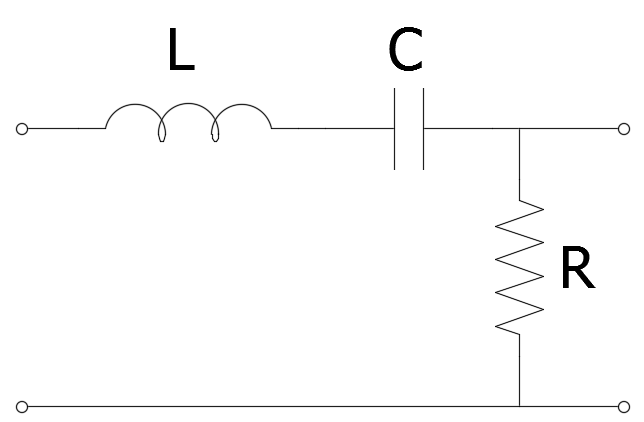
\includegraphics[width=0.3\textwidth]{img/theory/series_circ.PNG}
  	\caption{Exemplary circuit for series LC resonance.}
  	\label{fig:seriescircuit}
\end{figure}
\FloatBarrier

The impedance of such a circuit is as follows:

\begin{equation}
	Z=R+j\omega L+\dfrac{1}{j\omega C}
\end{equation}

In the case of series resonance, the total impedance at the resonance frequency is reduced exclusively to the resistive circuit component. Assuming $R=0$, the series resonance occurs at certain resonant frequency $f_r$, when the impedance is minimum i.e.:

\begin{equation}
	j\omega L+\dfrac{1}{j\omega C}=0
\end{equation}
What leads to:
\begin{equation}
	\omega_r=\dfrac{1}{\sqrt{LC}}
\end{equation}

Impedance magnitude of the system from Figure~\ref{fig:seriescircuit} and its angle is presented in the in the Figure~\ref{fig:seriesresonance}.

\begin{figure}[htb]
	\centering
    	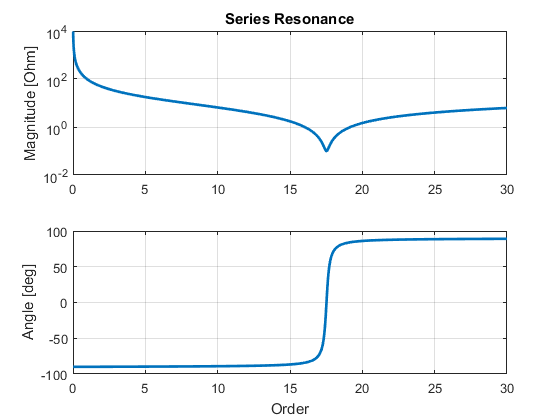
\includegraphics[width=0.7\textwidth]{img/theory/series_resonance_f876.png}
  	\caption{Series resonance in LC circuit at frequency 876 Hz ($17^{th} frequency order$).}
  	\label{fig:seriesresonance}
\end{figure}
\FloatBarrier

Since the impedance reduced for resonance frequency, the current can reach very high values:

\begin{equation}
	I_r=\dfrac{V_1}{R}=\dfrac{V_2}{R}
\end{equation}

Thus, we can see that the current is limited only by resistance. In the pure $LC$ case the currents tends to infinity and if $R$ is very small, current can be high.

\subsection{Parallel AC resonance}
The parallel resonance occurs in parallel RLC circuit (see the example circuit in the Figure~\ref{fig:parallelcircuit}) when the total impedance at the resonant frequency is very large (theoretically tends to infinite).

\begin{figure}[htb]
	\centering
    	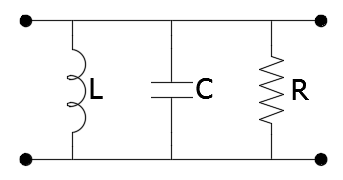
\includegraphics[width=0.3\textwidth]{img/theory/parallel_circ.png}
  	\caption{Circuit of parallel LC resonance.}
  	\label{fig:parallelcircuit}
\end{figure}
\FloatBarrier

\begin{equation}
	\dfrac{1}{Z}=\dfrac{1}{R}+\dfrac{1}{j\omega L+j\omega C}
\end{equation}

In this circuit, the resonant condition is (ignoring R - open-circuit):

\begin{equation}
	\omega C-\dfrac{1}{\omega L}=0
\end{equation}

Thus, the resonant frequency is as follows:

\begin{equation}
	\omega_r =\dfrac{1}{\sqrt{LC}}
\end{equation}

Exemplary impedance magnitude and angle plots of the system from Figure \ref{fig:parallelcircuit} are plotted at Figure \ref{fig:parallelresonance}.

\begin{figure}[htb]
	\centering
    	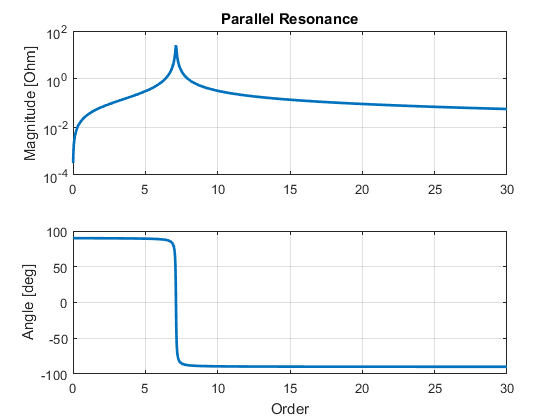
\includegraphics[width=0.7\textwidth]{img/theory/parallel_resonance_f356.png}
  	\caption{Parallel resonance in LC circuit at frequency 356 Hz ($7^{th} frequency order$).}
  	\label{fig:parallelresonance}
\end{figure}
\FloatBarrier

This condition may produce a large overvoltage between the parallel-connected elements, even under small harmonic currents. Therefore, resonant conditions may represent a hazard for solid insulation in cables and transformer windings and for the capacitor bank and their protective devices as well \cite{rosa}. 

\subsection{Tank circuit parallel AC resonance}
More practical LC circuit i.e. with inductor modelled with non-zero value of resistance and capacitor modelled without resistance is called Tank circuit \cite{das}. Figure~\ref{fig:tank} presents such a circuit.

\begin{figure}[htb]
	\centering
		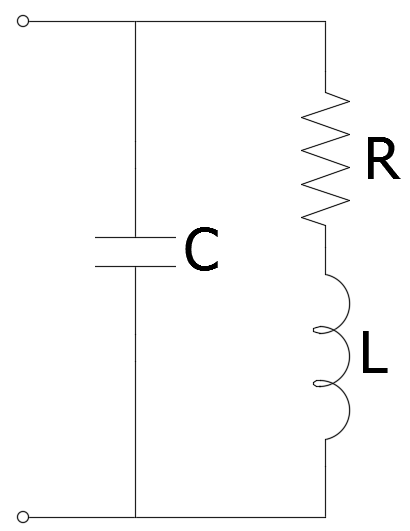
\includegraphics[width=0.2\textwidth]{img/theory/tank_circ.PNG}
	\caption{Tank circuit of parallel LC resonance.}
	\label{fig:tank}
\end{figure}
\FloatBarrier

In this circuit the aggregate admittance seen from the terminals is as follows:

\begin{equation}
	Y=j\omega C+\dfrac{1}{R+j\omega L}
\end{equation}

In other form:

\begin{equation}
	Y=\dfrac{R}{R^2+\omega^2L^2}+j\left(\omega C-\dfrac{\omega L}{R^2+\omega^2L^2}\right)
\end{equation}

The plot of exemplary impedance for such a system is presented in the Figure~\ref{fig:tankresonance}.

\begin{figure}[htb]
	\centering
		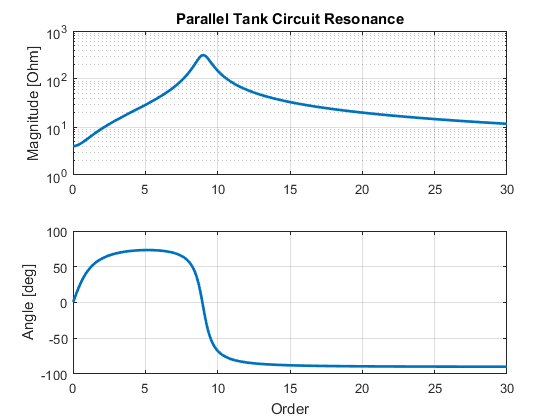
\includegraphics[width=0.7\textwidth]{img/theory/tank_parallel_resonance_f447.png}
	\caption{Parallel resonance in LC circuit at frequency 447 Hz ($9^{th} frequency order$).}
	\label{fig:tankresonance}
\end{figure}
\FloatBarrier

In the circuit with zero-resistance (lossless circuit), resonance occurs if impedance of inductor equals impedance of capacitor i.e. when the circuit works as short-circuited. In this case, resonance occurs in similar situation, even though the resistance stays unchanged in the circuit. In other words resonance occurs when power factor of admittance above equals zero \cite{das}.

\begin{equation}
	\omega C-\dfrac{\omega L}{R^2+\omega^2L^2}=0
\end{equation}

That gives resonance frequency:

\begin{equation}
	\omega_r=\sqrt{\dfrac{1}{LC}-\dfrac{R^2}{L^2}}
\end{equation}

Moreover, as distinct from the series resonance, where resonance can occur from any value of resistance, in this case resonance occurs only if following equation is true:

\begin{equation}
	\dfrac{R^2}{L^2}\leq \frac{1}{LC}
\end{equation}

In other words, resonance does not occur if:

\begin{equation}
	R>\sqrt{\dfrac{L}{C}}
\end{equation}

\subsection{Factors affecting resonance frequency in power system}
Generally speaking, in the power system, the following factors, by modification of network impedance, can impact resonance frequency values (based on \cite{das}):
\begin{itemize}
	\item Synchronous and asynchronous sources and loads in the power system. They can absorb some harmonics but also change the resonance points. Correct modelling of these elements is crucial.
	\item Impedance of the utility source. In models connected to such a source they are given by the three-phase short-circuit current, which corresponds to certain impedance.
	\item Shunt power capacitors. They are not recommended in presence of other devices producing harmonics. They shift resonance frequencies and can cause secondary resonance if applied at multi-voltage levels.
	\item Single phase loads. From impedance point of view, single phase loads are unsymmetrical loads, therefore lead to unsymmetrical phenomena.
	\item Already applied harmonic mitigating devices (e.g. passive filters). They does not remove the resonant conditions, but by introduction of new impedance, these devices only shift resonance frequency to the other level.
	\item Topology of the network. Any switching action will change the resonant frequency, since tha aggregated impedance of the network changes. 
\end{itemize}

\section{Effects of harmonics} \label{effectsofharmonics}
The harmonic resonance in a power system cannot be tolerated and must be avoided. The magnified harmonics will have serious effects on equipment heating, harmonic torque generation, nuisance operation of protective devices, derating of electrical equipment, damage to the shunt capacitors due to overloading, can precipitate shutdowns etc.

Some of the harmonic deleterious effects on electrical equipment are gathered in \cite{harmonicseffects}:
\begin{itemize}
	\item Capacitor bank failure because of reactive power overload, resonance, and harmonic amplification. Nuisance fuse operation.
	\item Excessive losses, heating, harmonic torques, and oscillations in induction and synchronous machines, which may give rise to torsional stresses.
	\item Increase in negative sequence current loading of synchronous generators, endangering the rotor circuit and windings.
	\item Generation of harmonic fluxes and increase in flux density in transformers, eddy current heating, and consequent derating.
	\item Overvoltages and excessive currents in the power system, resulting from resonance.
	\item Derating of cables due to additional eddy current heating and skin effect losses.
	\item Inductive interference with telecommunication circuits.
	\item Signal interference in solid-state and microprocessor-controlled systems.
	\item Relay malfunction.
	\item Interference with ripple control and power line carrier systems, causing misoperation of the systems, which accomplish remote switching, load control, and metering.
	\item Unstable operation of firing circuits based on zero-voltage crossing detection and latching.
	\item Interference with large motor controllers and power plant excitation systems.
	\item Possibility of subsynchronous resonance.
	\item Flickers.
\end{itemize}

\begin{comment}
\section{Nabe and Akagi instantaneous power theory}
Nabe-Akagi instantaneous reactive power $pq$ theory \cite{nabeakagi} is based on Clark’s transformations in three phase systems. 

The power in electrical circuit is described using instantaneous voltage and current without the use of Fourier series. Usually is used for switching compensators and active filters controls \cite{das}.

By linear transformation, the voltages $v_a ,v_b ,v_c$ and load currents $i_a ,i_b ,i_c$ are transformed into an $\alpha - \beta$ coordinate system. The instantaneous real power $p$ and the instantaneous imaginary power $q$ are defined on the basis of transformed voltages and currents. The following equations shows the transformations.

\begin{equation}
\begin{vmatrix}v_\alpha \\
v_\beta\end{vmatrix}=\sqrt{\frac{2}{3}}
\begin{vmatrix}
1 & -\frac{1}{2} & -\frac{1}{2} \\
1 & \frac{\sqrt{3}}{2} & -\frac{\sqrt{3}}{2}
\end{vmatrix}
\begin{vmatrix}
v_a \\v_b \\v_c 
\end{vmatrix}
\end{equation}

\begin{equation}
\begin{vmatrix}i_\alpha \\
i_\beta\end{vmatrix}=\sqrt{\frac{2}{3}}
\begin{vmatrix}
1 & -\frac{1}{2} & -\frac{1}{2} \\
1 & \frac{\sqrt{3}}{2} & -\frac{\sqrt{3}}{2}
\end{vmatrix}
\begin{vmatrix}
i_a \\i_b \\i_c 
\end{vmatrix}
\end{equation}

\begin{equation}
\begin{vmatrix}p \\
q\end{vmatrix}=
\begin{vmatrix}
v_\alpha & v_\beta \\
-v_\beta & v_\alpha
\end{vmatrix}
\begin{vmatrix}
i_\alpha \\i_\beta 
\end{vmatrix}
\end{equation}

On the basis of this theory, with further conversions of the equation we obtain the instantaneous active and reactive powers.

\begin{equation}
\begin{aligned}
	p=v_\alpha i_{\alpha p}+v_\beta i_{\beta p} \equiv P_{\alpha p}+P_{\beta p} \\
	p=v_\alpha i_{\alpha q}+v_\beta i_{\beta q} \equiv P_{\alpha q}+P_{\beta q}
\end{aligned}
\end{equation}

\begin{equation}
\begin{aligned}
	P_{\alpha p}=\frac{v_{\alpha}^{2}}{v_{\alpha}^{2}+v_{\beta}^{2}}p \\
	P_{\alpha q}=\frac{-v_{\alpha} v_{\beta}}{v_{\alpha}^{2}+v_{\beta}^{2}}q \\
	P_{\beta p}=\frac{v_{\beta}^{2}}{v_{\alpha}^{2}+v_{\beta}^{2}}p \\
	P_{\beta q}=\frac{v_{\alpha} v_{\beta}}{v_{\alpha}^{2}+v_{\beta}^{2}}q
\end{aligned}
\end{equation}

The powers $P_{\alpha p}$ and $P_{\beta q}$ cancels each other. Therefore, one can conclude that in the system of converter connected to source and load on both sides, there is no relationship between the instantaneous reactive power on the source side (between source and converter) and instantaneous reactive power on the load side (between converter and load). Thus, the instantaneous imaginary power on the input side is not equal to the instantaneous imaginary power on the output side. However, the instantaneous real power on the input side is equal to the real output power.
\end{comment}


\section{Park Transformation} \label{sec:park}
Park transformation is necessary to obtain the positive and negative impedances for converters equations presented in Section~\ref{sec:powerconverters-zs}.

Park transformation, also called dq0-transformation is a space vector transformation of three-phase time-domain signals from a stationary phase coordinate system ($abc$) to a rotating coordinate system ($dq0$) as follows \cite{park1929}:

\begin{equation}
\begin{bmatrix}
u_d\\ 
u_q\\
u_0
\end{bmatrix}=
\frac{2}{3}\begin{bmatrix}
cos(\Theta) & cos(\Theta-\frac{2\pi}{3}) & cos(\Theta+\frac{2\pi}{3})\\ 
-sin(\Theta) & -sin(\Theta-\frac{2\pi}{3}) & -sin(\Theta+\frac{2\pi}{3})\\ 
\frac{1}{2} & \frac{1}{2} & \frac{1}{2}
\end{bmatrix}=
\begin{bmatrix}
u_a\\ 
u_b\\
u_c
\end{bmatrix}
\end{equation}

where $\Theta=\omega t+\delta_A$ is the angle between the rotating and fixed coordinate system at each time $t$ and $\delta_A$ is an initial phase shift of the voltage.

The inverse transformation from the $dq0$ frame to the $abc$ frame:

\begin{equation}
\begin{bmatrix}
u_a\\ 
u_b\\
u_c
\end{bmatrix}=
\begin{bmatrix}
cos(\Theta) & -sin(\Theta) & 1\\ 
cos(\Theta-\frac{2\pi}{3}) & -sin(\Theta-\frac{2\pi}{3}) & 1\\ 
\cos(\Theta+\frac{2\pi}{3}) & -sin(\Theta+\frac{2\pi}{3}) & 1
\end{bmatrix}=
\begin{bmatrix}
u_d\\ 
u_q\\
u_0
\end{bmatrix}
\end{equation}

\chapter{Harmonics analysis methods} \label{sec:methodsofanalysis}
In this study we focus on the methods of analysis in frequency-domain like the ones described below. Therefore methods of harmonic analysis in time-domain like Fourier Series, Discrete Fourier Transform (DFT) or Fast Fourier Transform (FFT) etc. are not included in this description.

The phenomenon of harmonic resonance seems well understood in the literature, however tools available to analyse it are very limited \cite{xu2005}. Method of frequency scan (frequency sweep) is the most general and common method to identify the resonance frequencies in networks \cite{modal1982}. However, this method is limited. The resonance is between two elements (capacitive and inductive) in the system and networks usually consists of many elements. The result of frequency sweep does not indicate which elements exchange energy between each other, causing resonance.

The method of Harmonic Resonance Modal Analysis (HRMA) was developed to face this problem \cite{xu2005}. This method involves only analysis of parallel resonance which is more dangerous in the power system. From HRMA the buses which excite a particular resonances can be identified. Thus, we can observe which components are more involved in a resonance than other. From these results we can conclude where a resonance can be observed more easily or how far the resonance can propagate in the system \cite{xu2005}.

\section{Frequency Sweep} \label{sec:theoryfs}
Frequency Sweep (or Frequency Scan) analysis is a characterization of the system equivalent impedance at a bus in the system as a function of frequency \cite{bradt2012}. As the result, curve of impedance in frequency domain is obtained. The peaks in the curve suggest frequencies when parallel resonance occurs (very high impedance at certain frequency) while dips indicate the frequencies when series resonance occurs (very low impedance at certain frequency). 

In Wind Power Plants frequency scans are often done at various grid locations or at the collector bus \cite{bradt2012}. The magnitude of computed impedances depends also on the level of equivalent voltage used in the calculations. However, the single value of identified peak impedance does not determine if a dangerous harmonic resonance occurs. For harmonic problems, there must also be a sufficient level of harmonic source voltages or currents at or near the resonant frequency to excite harmonic resonance \cite{bradt2012}. Also, the impedance value itself has to be analysed in particular case to identify the value that could cause harm. To do this, the best way is to obtain specific data by measurements, but also data provided by manufacturers of devices in the network.

\section{Harmonic Resonance Modal Analysis} \label{sec:theoryhrma}
The method is based on analysis of well-known admittance matrix - $\bm{Y}$. It focuses on the large elements of inverted $\bm{Y}$. In the extreme case (very large elements) the admittance matrix tends to singularity and element of inverted $\bm{Y}$ tends to infinity, thus very high voltages can be produced, which is in principle parallel resonance.

The elements are identified on the basis of eigenvalues of $\bm{Y}$ matrices. Since matrix becomes singular when even one of the eigenvalue becomes zero, the principle can be clearly used. Eigenvalues correspond to certain mode of harmonic resonance, therefore the study consists of identification of critical resonance modes. The equations describing the method including the identification of certain buses and elements are presented below.

The admittance matrix on the network is constructed for certain frequency $\bm{Y_f}$. Admittance matrix fulfils equation:
\begin{equation}
	\bm{V_f=Y_f^{-1}I_f}
\end{equation}
where: $\bm{Y_f}$ is the network admittance matrix $\bm{V_f}$ is the nodal voltage and $\bm{I_f}$ is the nodal current injection. All matrix values are at frequency $f$.

To investigate if $\bm{Y_f}$ approaches singularity, the theory of eigen-analysis is applied. According to \cite{bellman1970}, matrix $\bm{Y_f}$ can be decomposed into (index $f$ is neglected in the next equations for simplicity):

\begin{equation} \label{eq:hrma1}
	\bm{Y=L\cdot\Lambda\cdot T}
\end{equation}

where $\bm{\Lambda}$ is the diagonal eigenvalue matrix and $\bm{L}$ and $\bm{T}$ are the left and right eigenvector matrices.

Defining $\bm{U=TV}$ as the modal voltage vector and $\bm{J=TI}$ as the modal current vector, the equation can be derived:

\begin{equation}
	\bm{U=\lambda^{-1}J}
\end{equation}

or

\begin{equation}
	\begin{bmatrix}
		U_1\\ 
		U_2\\ 
		...\\ 
		U_n
	\end{bmatrix}
	=
	\begin{bmatrix}
		\lambda_1^{-1}&0&0&0\\ 
		0&\lambda_2^{-1}&0&0\\ 
		0&0&...&0\\ 
		0&0&0&\lambda_n^{-1}  
	\end{bmatrix}
	=
	\begin{bmatrix}
		J_1\\ 
		J_2\\ 
		...\\ 
		J_n
	\end{bmatrix}
\end{equation}
where each $\lambda^{-1}$ has the unit of impedance and is named modal impedance $Z_m$. From matrix Equation~~\ref{eq:hrma1}, one can easily identify the “location” of resonance in the modal domain due to corresponding modal currents and voltage. If $\lambda_1=0$ or is very small, a small injection of modal 1 current $J_1$ will lead to a large modal 1 voltage $U_1$ \cite{xu2005}. Thus, we can identify that a resonance takes place for specific mode (or modes) and it is not related to a particular bus injection since the values are in modal domain. The smallest eigenvalue is called the critical mode of harmonic resonance and its left and right eigenvectors are the critical eigenvectors.

The modal currents $J$ are a linear projections of the physical currents in the direction of the first eigenvectors by: $\bm{J=TI}$. Also the physical nodal voltages are related to the modal voltages by: $\bm{V=LU}$. More details in \cite{xu2005}. In summary, the critical eigenvectors characterize the excitability of the critical mode (right critical eigenvector) and observability of the critical mode (left critical eigenvector). The excitability and observability of modes are characterized with respect to the location. 

It is also possible to combine the excitability and observability into a single index according to the theory of selective modal analysis \cite{perez1982}:

\begin{equation} \label{eq:hrma2}
	\bm{V=L\Lambda^{-1}TI}
\end{equation}

However, this approximation is made possible because $1/\lambda_1$, the critical modal impedance, is much larger than the other modal impedances. If there are more impedances at the similar level as critical impedance, we will observe some inaccuracies in the results.

Assuming one critical modal impedance, much larger than the others, the diagonal elements of the above matrix $\bm{LT}$ characterize the combined excitability and observability of the critical mode at the same bus. They are called participation factors (PF's) of the bus and are defined as follows \cite{xu2005}:

\begin{equation} \label{eq:hrma3}
	PF_{bm}=L_{bm}\cdot T_{mb}
\end{equation}

where $b$ is the bus number and $m$ is the mode number.

From the calculation on the basis of admittance matrix and the  approximation above (Equations~\ref{eq:hrma1} - \ref{eq:hrma3}) we obtain: the set of participating factors for each bus for each critical mode (the modes when the modal impedance peaks), which occurs for certain frequency at certain number of mode. Moreover, if approximation of only one critical impedance is right, the participation factors of all buses sum up to 1, therefore the comparison of participation factors between buses is simple and we express them in percentage values.

\section{Critical Modes and Resonance Condition – comparison between FS and HRMA}
As mentioned, resonant conditions identified in this method depends on the value of eigenvalue, which is very small if resonance occurs. This is equal in other words to very high modal impedance. As seen from comparison with frequency scan impedance curves, the sharp peaks occur for the same frequencies. One has to remember that in frequency scan method, the impedance curves are seen from the certain point in the grid, while in HRMA the impedance curves are divided into modes, which does not correspond exactly to the physical buses, even though the number of modes and the number of buses is the same.

Moreover the values of maximum impedances at peak point from both methods are different. The reason is again due to comparison between \textit{real} impedance and \textit{modal} impedance. Modal impedance should be investigated referring to every specific case in order to identify the threshold value or the range, above which the harmful resonance occurs. In this study, values of interests identified by both methods are the frequencies when resonances occurs, therefore the harmful impedance, neither real nor modal are not identified.

\chapter{Harmonics in Wind Power Plant} \label{sec:harmonicsinwpp}
Wind Power Plants, due to intermittency of the wind, are usually supported by great number of power electronic converters which enable effective operation of WPP. These non-linear devices are sources of significant amounts of harmonics in Wind Farms. 

Harmonics produced by converters first of all are introduced into inner grid of WPP. Before any waveform produced by wind turbines and converted by wind turbines converters is introduced into the power system (through PCC between WPP and external grid), it is exposed to dangerous phenomenon of harmonic resonance in inner grid of WPP. 

Internal harmonic resonance depends essentially on the elements that the inner grid consists of (including possible HVDC link converter) and the way of their connection (topology). As described in Section~\ref{sec:harmonicresonance} harmonic resonance contributes to amplification of existing harmonics and is able to create new harmonic components.

As the result, overall external emission of harmonics (to the power system) from Wind Power Plants, if the WPP is not decoupled by HVDC link, first of all depends on \cite{das} (i) converter topology, (ii) applied harmonic filters and (iii) short-circuit current at PCC. These three features has to be completed by the above problem of (iv) internal harmonic resonance in the WPP inner grid. If the wind farm is connected by HVDC link, then the emission of harmonics to the external grid depends on the DC/AC conversion at the PCC behind HVDC connection. Even though, the emission to the grid of such a WPP is not a problem, harmonic phenomena still creates a many issues in the inner WPP AC grid.

\textit{Main focus of the thesis is understanding and description harmonic resonance appearing in inner grids of Wind Power Plants. Moreover, stability issues due to the harmonic resonance are put forward. As mentioned in the Section \ref{sec:motivation}, the analysis of these problems has recently become very important due to serious problems observed in first HVDC connected offshore wind farm during its first years of operation. For future implementation of HVDC connected offshore WPP the problem is currently investigated.}

\section{Converter topology in WPP}
Topology of WT-converters in WPP's is partially determined by the electrical machine that is used in wind turbine to generate electricity. According to the level of power that flows through a converter, full scale converter can be distinguished. It provides control over total power produced in generator. On the other hand, there are also Wind Turbine application where only part of the power produced can flows through converter. The ratings of the converter, so also its costs, are reduced, however control of the power produced in wind turbine is limited. 

Within the full-scale converters, the most popular utilized in these days in wind turbines are: 2-level converters, 3-level NPC converters, multi-level converters, also matrix converters and tandem converters \cite{pham2013}.

Regarding the harmonics propagation problem from each WT-converter, when it comes to the scale of the wind farm, as stated in \cite{das}, the greater the number of turbines the lower is the magnitude of the harmonics and subharmonics, especially of the lower order.

In this study, only models of full rate wind turbine converters are considered. On the other hand, HVDC link converter is modelled with respect to principles described in the Section~\ref{sec:powerconverters}.

\section{Control of harmonics and harmonic resonance}
The two main methods for controlling harmonics in WPP are avoiding producing of harmonics and implementing filters to mitigate them \cite{bradt2012}. To avoid the production of harmonics, network of WPP has to be designed properly, however implementation of harmonic filters anyway can be necessary due to topology changes or even very insignificant modifications which change resonance levels. The designing of filters should be based on measurements and simulations in order to control resonance properly.

Second method - implementation of filters - is the most common approach to the harmonic resonance \cite{bradt2012}. The design and implementation of filters is not considered in this study, however the HRMA method presented is crucial for identification of the buses which are potentially more appropriate for filters implementation.

\section{Short circuit current at PCC}
From the main grid side, the short circuit level at the point of application is also not fixed. It varies with operational condition in the grid. The weaker the external grid, the more it varies usually, therefore the resonant frequency can float around. These fluctuations are not considered in the thesis.

\section{Internal WPP resonance}
The phenomenon of electrical resonance is described in section \ref{sec:harmonicresonance}. As mentioned, if the resonance is not properly controlled, it leads to failures, instabilities, shut-downs or even damage of components. If the internal grid of WPP is separated from external grid for example by HVDC connection, electrical behaviour of the WPP grid can be different from the main grid.

In such a WPP inner grid there is no rotating mass that establishes physical binding of power and frequency \cite{borwin1}. Thus, the frequency of internal WPP and the infeed from the WTs can and should be completely controlled by converters. Moreover, every converter has its own control schemes that can have a bandwidth of several hundred hertz. Thus, converters are able to amplify oscillations which are in the system \cite{borwin1}.

\textit{The resonance in Wind Power Plant is the main reason of the instability in first HVDC connected offshore WPP, described in motivation part of the thesis (section~\ref{sec:motivation})}.

\chapter{Stability of WPP}
In VSC converters the bandwidth of control signals are several times of the fundamental frequency. Such high-frequency control introduces dynamics above fundamental frequency, creating potential for high frequency instabilities and resonances that are not present in CSC \cite{liusun2014}. Since the VSC does not need reactive power support, has higher controllability and the ability of black start the system, this type of converter is getting more popular in new Wind Farms.

In the offshore WPP Bard Offshore 1 VSC converters are utilized \cite{borwin1}. However the problem of grid resonances caused by these converters was not considered during planning phase of the WPP. Therefore, stability problems due to converters interactions were not considered.

As stated in \cite{sun2011} and \cite{liusun2014} converters could go into resonance with the grid causing instabilities if the grid impedance exceed the input impedance of the converter. On the basis of this statement, the analysis of stability is performed. The essence of the method is presented in \cite{middlebrook1976}. Stability problems happen due to more advanced nonlinear power electronics included in the converters. The problem of modelling converter impedance nonlinear behaviour is described in Section~\ref{sec:powerconverters-zs}. This sort of problems does not occur between, for example, synchronous generators since power electronic elements influence in these elements is limited.

\section{Harmonic Stability}
The stability criterion based on Nyquist stability criterion is described in \cite{sun2011} and is still under development \cite{borwin1}. The main advantage of this method is that it does not require all details about converter which are always considered as intellectual property of manufacturers. Due to this advantage it could be right choice at the planning phase of an investment. Only frequency dependent impedances of converter are needed \cite{borwin1}. The method also avoids the need to remodel each inverter and repeat its loop stability analysis when the grid impedance changes \cite{sun2011}.

In contrast to EMT simulations and eigenvalue analysis only relatively simple stability criterion is developed. Thus, this method is very fast and can evaluate new topology if any switching action occurs \cite{borwin1}. The simplicity is achieved by aggregation of all wind farms with their controllers into one element. Then, the aggregated system is evaluated by Nyquist stability criterion that provides information about gain and phase margin. As mentioned, the manufacturers have to provide only frequency dependent impedance of their generation unit (converter), including passive elements impedance and impedance changes due to active controls. In other words, the main advantage of this approach is that the frequency dependent impedance can be calculated with analytic model (providing appropriate data from manufacturer) or calculated with an EMT-tool but also measured at a real generation unit \cite{borwin1}.

\section{Impedance-based stability evaluation model} \label{sec:stabilitymodel}
With the proper data and assumptions described above, we use the simple model to evaluate the stability consisting of voltage source with internal impedance and the impedance of the grid (Figure~\ref{fig:stabilitymodel1}) \cite{sun2011, borwin1}.

\begin{figure}[htb]
	\centering
    	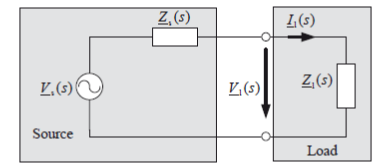
\includegraphics[width=0.5\textwidth]{img/theory/stability_model1.png}
  	\caption{Stability analysis first model.}
  	\label{fig:stabilitymodel1}
\end{figure}
\FloatBarrier

In such a network the current $I_g$ depends on both $Z_s$ and $Z_g$ impedances:

\begin{equation} \label{eq:stab1}
	I_g=\dfrac{V_s (s)}{Z_s (s)+Z_g (s)}=\dfrac{V_s (s)}{Z_g (s)} \dfrac{1}{1+\dfrac{Z_s (s)}{Z_g (s)}}
\end{equation}

The equation of the network $_Ig$ current (Eq.~\ref{eq:stab1}) can be expressed in as loop gain for the system in the Figure~\ref{fig:stabilityloop}.

\begin{figure}[htb]
	\centering
    	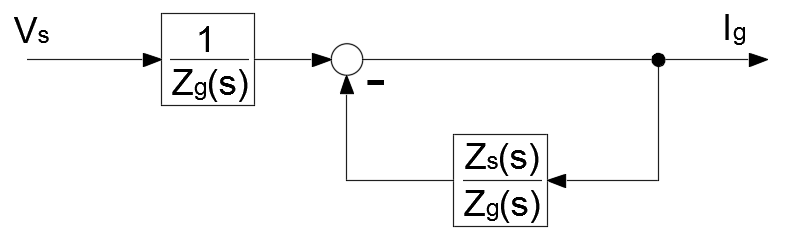
\includegraphics[width=0.5\textwidth]{img/theory/stability_loop.png}
  	\caption{Loop gain corresponding to the stability model.}
  	\label{fig:stabilityloop}
\end{figure}
\FloatBarrier

On the basis on the equation (Eq.~\ref{eq:stab1}) we conclude that the system is stable if the source has a zero and the load an infinite output impedance. For stability, the value of ratio $|Z_s (s)/Z_g (s)|$ has to be at least below 1 to for all frequencies \cite{sun2011} – in other words – the system is table if  $Z_s (s)/Z_g (s)$ satisfies the Nyquist stability criterion \cite{middlebrook1976}.

The first problem with the model above is the point division between $Z_s$ and $Z_l$. The best point of division is still under investigation \cite{borwin1}. In this study the network is divided behind the HV transformer from the HVDC link point of view (Bus 2) (see Figure~\ref{fig:systemcase3}).

There is also other conceptual problem with the presented approach. As either the inverter of WT of HVDC inverter could be treated as the source, the results about stability conclusions are very different \cite{sun2011}. In this study we perform only one approach where the aggregated WT converter is treated as “source” and HVDC link converter as “grid” and the point of division is always as described above.

Finally, the stability criterion requires frequency impedances of converters which could be modelled as either voltage or current sources. The problems and details about these two models are explained in \cite{sun2011}. The “source” part and the “grid” part of the network can be modelled by its Thevenin equivalent circuit (voltage source) or Norton equivalent circuit (current source). 
The Thevenin model for stability criterion was presented above. However, it is also possible to represent converters by current source \cite{sun2011} (Figure~\ref{fig:stabilitymodel2}).

\begin{figure}[htb]
	\centering
    	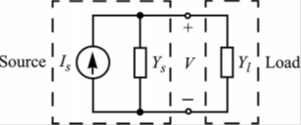
\includegraphics[width=0.5\textwidth]{img/theory/stability_model2.png}
  	\caption{Stability analysis second model.}
  	\label{fig:stabilitymodel2}
\end{figure}
\FloatBarrier

The stability criterion is, analogically to (Eq.~\ref{eq:stab1}), based on the system equation:

\begin{equation} \label{eq:stab2}
	V(s)=I_s (s)Z_g (s) \dfrac{1}{1+Z_s (s)/Z_g (s)}
\end{equation}

where, for stability, the ratio of the load input impedance to the source output impedance should meet the Nyquist stability criterion.

Comparing (Eq.~\ref{eq:stab1}) to (Eq.~\ref{eq:stab2}) one can see that stability requirement for CS system is opposite to that for VS system. The distinction between these models is described in \cite{sun2011}. The author states also that the most common grid model is hybrid system combining current and voltage sources (Figure~\ref{fig:stabilitymodel3}). Applying hybrid model to the case of this study, the wind turbine inverter is modelled as a current source while, the HVDC rectifier is modelled as voltage source.

\begin{figure}[htb]
	\centering
    	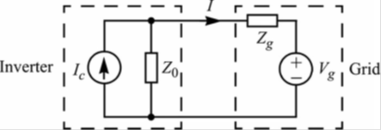
\includegraphics[width=0.5\textwidth]{img/theory/stability_model3.png}
  	\caption{Stability analysis hybrid model.}
  	\label{fig:stabilitymodel3}
\end{figure}
\FloatBarrier

The assumptions of the stable system without the inverter and the stable inverter when grid impedance is zero are still applicable.

Then, the current in the system is:

\begin{equation} \label{eq:stab3}
	I(s)=\left [ I_s(s)-\frac{V_g (s)}{Z_s (s)} \right ]\cdot \frac{1}{1+Z_g (s)/Z_s (s)}
\end{equation}

and the Nyquist stability criterion of this system is: $Z_g (s)/Z_s (s)$.

\section{Stability assessment} \label{sec:stabilityassessment}
From the examples and assumptions described above, we assess the stability \textit{source} and \textit{grid} are plotted in a Bode diagram for positive and negative sequences. From Bode diagram, each intersection of grid curves with source curves could be critical and has to be investigated. For each intersection, phase margin between appropriate curves (curves that intersects) will be calculated according to:

\begin{equation}
	\phi_m =180\degree-\Delta \phi
\end{equation}

where $\Delta \phi$ is the phase difference between curves in degree. If the phase margin calculated in such a way is below $30\degree$ the system can be instable \cite{borwin1}. As aforementioned the stability assessment is performed for specified point of division and specified \textit{source} and \textit{grid} sides.

\chapter{Modelling of elements} \label{sec:modellingofelements}
\section{Transformers}
For harmonics modelling of transformers in electrical grid models for very high frequencies a generally not necessary. For higher frequencies resistance increases, while the leakage inductance reduces \cite{das}. In this study, two- and three- winding transformers impedances will be represented simply by its resistance and inductance as follows:

\begin{equation}
	Z_{tr}(f)=R_{tr}+jX_{tr} (f_h/f_1 )
\end{equation}

where $R_tr$ and $X_tr$ correspond to fundamental frequency resistance and reactance. The skin effect and eddy currents effect the resistance at higher frequencies, therefore we do not consider these effects.

\section{Cables}
Modelling of cables is important in harmonic analysis since they are very significant source of capacitance in considered grids. For harmonic frequencies up to 3000Hz the resistance of cables will increase. The slight effect of decrease in inductance and shunt capacitance can be ignored \cite{das}. PI models are considered as appropriate for frequency scan analysis, but not for transient analysis.
Usually, exact frequency-dependent model is obtained by Finite Element analysis \cite{das}, however in this study exact methods of cable models are not considered. Elements of Pi model of the cables is described by:

\begin{equation}
\begin{aligned}
	Z_{cable} (j\omega_f)=R_{cable}+j(\omega_f/\omega_1 ) L_{cable}
\\
	Y_{cable} (j\omega_f)=j(\omega_f/\omega_1 ) C_{cable}
\end{aligned}
\end{equation}

\begin{figure}[htb]
	\centering
    	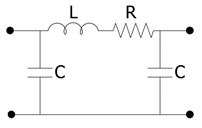
\includegraphics[width=0.3\textwidth]{img/theory/pi_model.png}
  	\caption{PI model circuit of the cables.}
  	\label{fig:pimodel}
\end{figure}
\FloatBarrier

\section{Filter reactors}
Filter reactors modelling is important since it significantly affects the tuning of whole system. Resistance of the filters at high frequencies can be calculated as follows:
\begin{itemize}
	\item For aluminium reactors: $R_h=\left [ \frac{0.115h^2+1}{1.15} \right ] R_f$
	\item For copper reactors: $R_h=\left [ \frac{0.015h^2+1}{1.055} \right ] R_f$
\end{itemize}
In the models presented, series resistance of LCL filters and resistance of phase reactor is neglected (equals zero).

\section{Power converters} \label{sec:powerconverters}
Modelling of power converters is the most crucial and challenging within all elements. Power converters devices are very nonlinear and their impedance behaviour strongly depends on many factors. The exact model should be derived on the basis of control codes, ideally also on the basis of measurements on the real device.

Control codes are very unique and never published by the manufacturers. Control codes are considered their intellectual property and thus the determination of the exact frequency is very difficult \cite{borwin1}. There are also more simple approaches to face the problem of converter modelling. The principles presented below are considered for frequency domain analysis. EMT (electromechanical transient) analysis is not considered.

\subsection{Voltage Source  (VS) and Current Source (CS) models} 		\label{sec:powerconverters-vscs}

\begin{figure}[htb]
	\centering
    	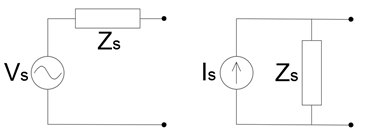
\includegraphics[width=0.5\textwidth]{img/theory/vscsmodels.png}
  	\caption{Ideal voltage and current source models.}
  	\label{fig:vscsmodels}
\end{figure}
\FloatBarrier

It is common to approach modelling of converters as either current or voltage source. As stated in \cite{borwin1}, current sources should be only used if the grid impedances are similar. Otherwise it leads to very inaccurate harmonic current values and wrong results. Therefore, voltage sources should be modelled instead and the input impedance should be considered.

There is very important fact to be considered for both approaches in frequency domain analysis. According to circuit theory, ideal voltage source internal resistance is zero (short-circuit). On the other hand, the ideal current source internal resistance is infinite (open-circuit).

In this study, models with either ideal current source or voltage sources are considered for comparison in FS method and HRMA method. For those models, internal impedance of source (VS or CS) $Z_s$ is zero or infinite, respectively. The third model of converter is described in the following section and is based on voltage source with nonzero, nonlinear internal impedance $Z_s$ (nonideal VS). For stability study the principles of converters modelling and stability assessment are described in Sections~\ref{sec:stabilitymodel}-\ref{sec:stabilityassessment}.

\subsection{Frequency dependent impedance model “Z(s)”}  \label{sec:powerconverters-zs}

The models of either voltage source or current source described in the previous section are very important, however for the resonance analysis the value of series impedance (in case of voltage source) or parallel impedance (in case of current source) is crucial. The voltage and current sources themselves should be open-circuited or short-circuited, respectively. The approach developed in \cite{liusun2014} and \cite{liusun2013} of frequency dependent impedance of converters is introduced to this study and described below.

The authors, by applying appropriate modelling method, such as harmonic linearization presented in \cite{sun2009linearization, bing2009}, obtain impedance models valid below and above the fundamental frequency \cite{liusun2014}. Each converter is described by positive- and negative-sequence impedances without cross coupling \cite{cespedes2014}. The Park's transformation, described in Section~\ref{sec:park} is also crucial to derive the converters impedances equations.

The assumed converters modelled are \cite{liusun2014}: 2-level VSC Wind Turbine DC/AC inverter and the same type of HVDC AC/DC rectifier. Models of these converters are then used in the simulation.

\subsubsection{Wind turbine converter (inverter)}
For the control purposes, wind turbine converter is controlled as current source. Due to this fact, the device behaves more like current source and the control will be modelled in this way. Reactive power supply and voltage regulation of the model is not considered. A phase-locked loop (PLL) is included in the model for AC bus synchronisation \cite{liusun2014}.

\begin{figure}[htb]
	\centering
    	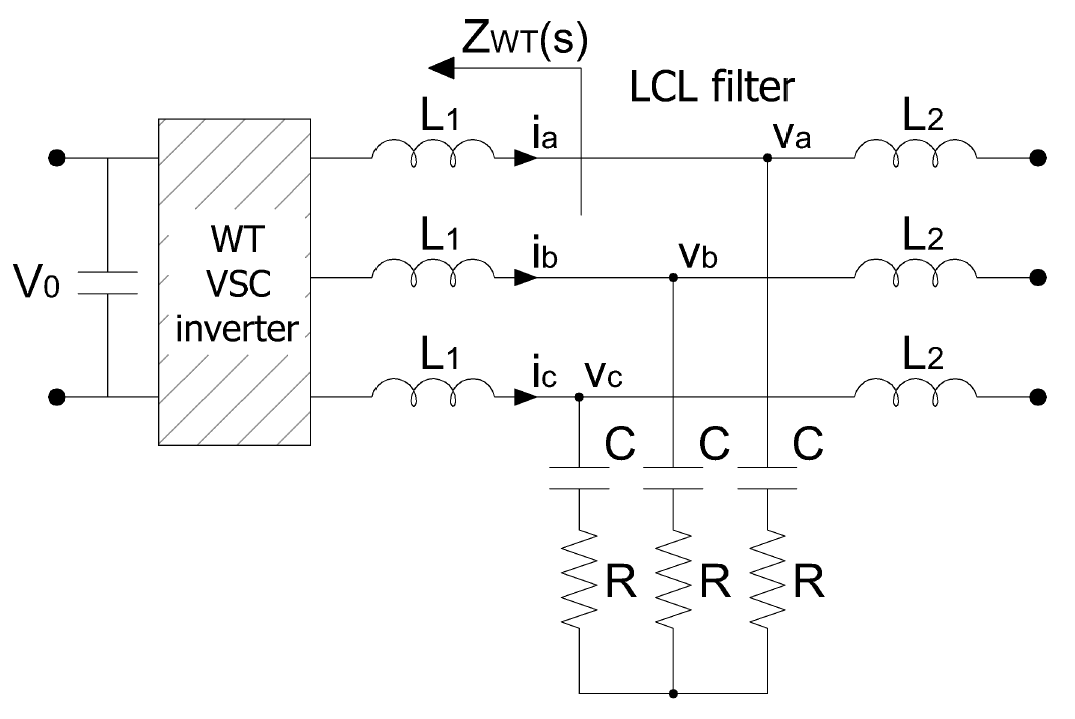
\includegraphics[width=0.6\textwidth]{img/theory/WT_scheme.png}
  	\caption{Aggregated wind turbine converter impedance model.}
  	\label{fig:wtscheme}
\end{figure}
\FloatBarrier

The wind turbine model is described in $dq$-frame. As mentioned, the current control scheme is used. The reference value is the current provided be the DC link voltage regulator. The current compensator transfer function is given:

\begin{equation}
	H_i (s)=K_p +\dfrac{K_i}{s}
\end{equation}

The PLL is implemented using PI regulator. Including the integrator to convert frequency into angle, the PLL compensation transfer function becomes:

\begin{equation}
	H_p (s)=\left ( K_p +\dfrac{K_i}{s} \right )\dfrac{1}{s}
\end{equation}

The values of parameters are specified in Chapter.

For the stability study, the wind turbines are lumped into one device (one impedance). The output impedance of WT inverter is developed using the harmonic linearization method described in \cite{bing2009}. As the result, converters are represented by positive-sequence and negative-sequence impedances without cross coupling \cite{cespedes2014}. Providing constant DC bus voltage (as the reference) the impedances become:

\begin{equation} \label{eq:impedance_wt}
\begin{aligned}
	Z_p (s)=\frac{H_i (s-j\omega_1)V_0 +(s-j\omega_1)L_1 }{1-T_{pll} (s-j\omega_1)[1+H_i (s-j\omega_1)I_1 V_0 /V_1 ]} \\
	Z_n (s)=\frac{H_i (s-j\omega_1)V_0 +(s-j\omega_1)L_1 }{1-T_{pll} (s-j\omega_1)[1+H_i (s-j\omega_1)I_1 V_0 /V_1 ]}
\end{aligned}
\end{equation}
where $\omega_1$ is fundamental angular frequency, $T_pll (s)$ is the loop gain of $dq$-frame PLL defined by:
\begin{equation}
	T_{pll} (s)=\dfrac{V_1 H_p (s)}{2[1+V_1 H_p (s)]}
\end{equation}

and $H_i$ and $H_p$ are the current an PLL compensator transfer functions, as defined before.

\subsubsection{HVDC link converter (rectifier)}
In case of HVDC converter, the device is controlled to behave as a voltage source at the ac terminals \cite{larsen2012}. Figure~\ref{fig:hvdcscheme} demonstrate the model for HVDC converter impedance calculation.

\begin{figure}[htb]
	\centering
    	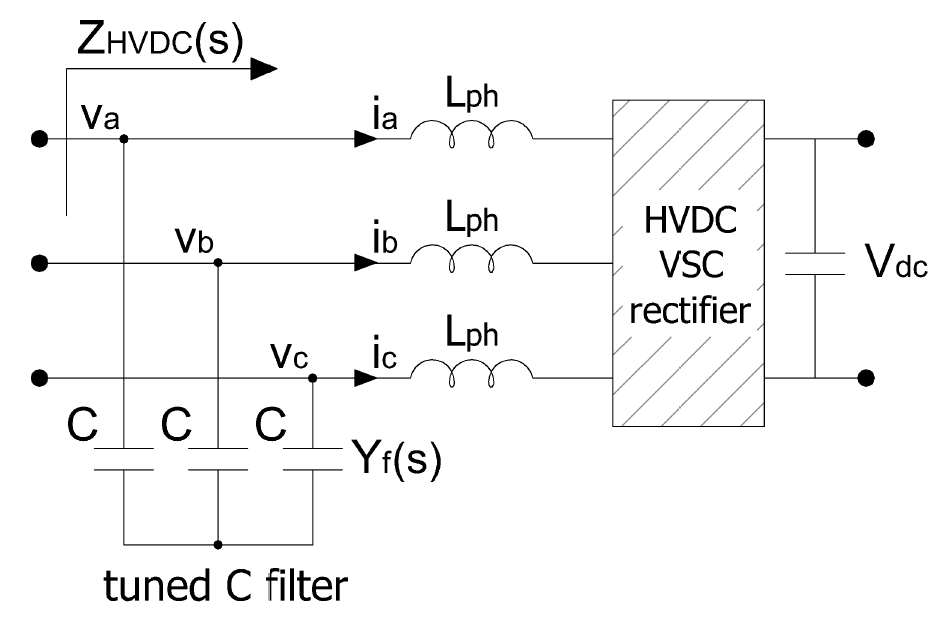
\includegraphics[width=0.6\textwidth]{img/theory/HVDC_scheme.png}
  	\caption{HVDC-link converter impedance model.}
  	\label{fig:hvdcscheme}
\end{figure}
\FloatBarrier

The HVDC rectifier voltage control is performed by a PI regulator in the dq-reference frame \cite{liusun2014}:

\begin{equation}
	H_v (s)=K_p +\dfrac{K_i}{s}
\end{equation}

A current loop is embedded within the voltage loop and the current compensator transfer function is defined as:

\begin{equation}
	H_i (s)=K_p +\dfrac{K_i}{s}
\end{equation}

Other control approaches could be incorporated but are not considered. The values of parameters are included in Chapter II.

Again, the assumption of constant DC-link voltage ($V_dc$) is made. The resulting positive- and negative-sequence input impedance are given by:

\begin{equation} \label{eq:impedance_hvdc}
\begin{aligned}
	Z_p (s)=\frac{H_i (s-j\omega_1)V_{dc} +sL_{ph}}{1+Y(s)[H_i (s-j\omega_1 )V_{dc} +sL_{ph} ]+T_p (s)} \\
	Z_n (s)=\frac{H_i (s+j\omega_1)V_{dc} +sL_{ph}}{1+Y(s)[H_i (s+j\omega_1 )V_{dc} +sL_{ph} ]+T_n (s)}
\end{aligned}
\end{equation}

where $\omega_1$ is fundamental angular frequency, $Y(s)$ is admittance of the ac filter, in our case equals $Y(s)=sC$. $T_p (s)$ and $T_n (s)$ are defined as:

\begin{equation}
\begin{aligned}
	T_p (s)=[H_i (s-j\omega_1 )+jK_{id} ]H_v (s-j\omega_1 )V_{dc} \\
	T_n (s)=[H_i (s+j\omega_1 )-jK_{id} ]H_v (s+j\omega_1 )V_{dc}
\end{aligned}
\end{equation}
and $H_i (s)$ and $H_v (s)$ are the current and voltage compensator transfer functions defined before.

Implementation of equations above is described in Section~\ref{sec:convertersmodels}, where we present necessary data and evaluate results.

\chapter{Simulations} \label{ch2}

\section{System description}
In most of the simulations for harmonic resonance study we consider offshore wind power plant with VSC-HVDC connection to the onshore grid. Total amount of installed wind turbines power is 400MW. The WPP considered has a radial topology consisting of four-branch network. It is assumed that each string (branch) of wind turbines has the same parameters. The layout of the 400MW WPP is presented in the Figure~\ref{fig:systemfull}.

\begin{figure}[htb]
	\centering
	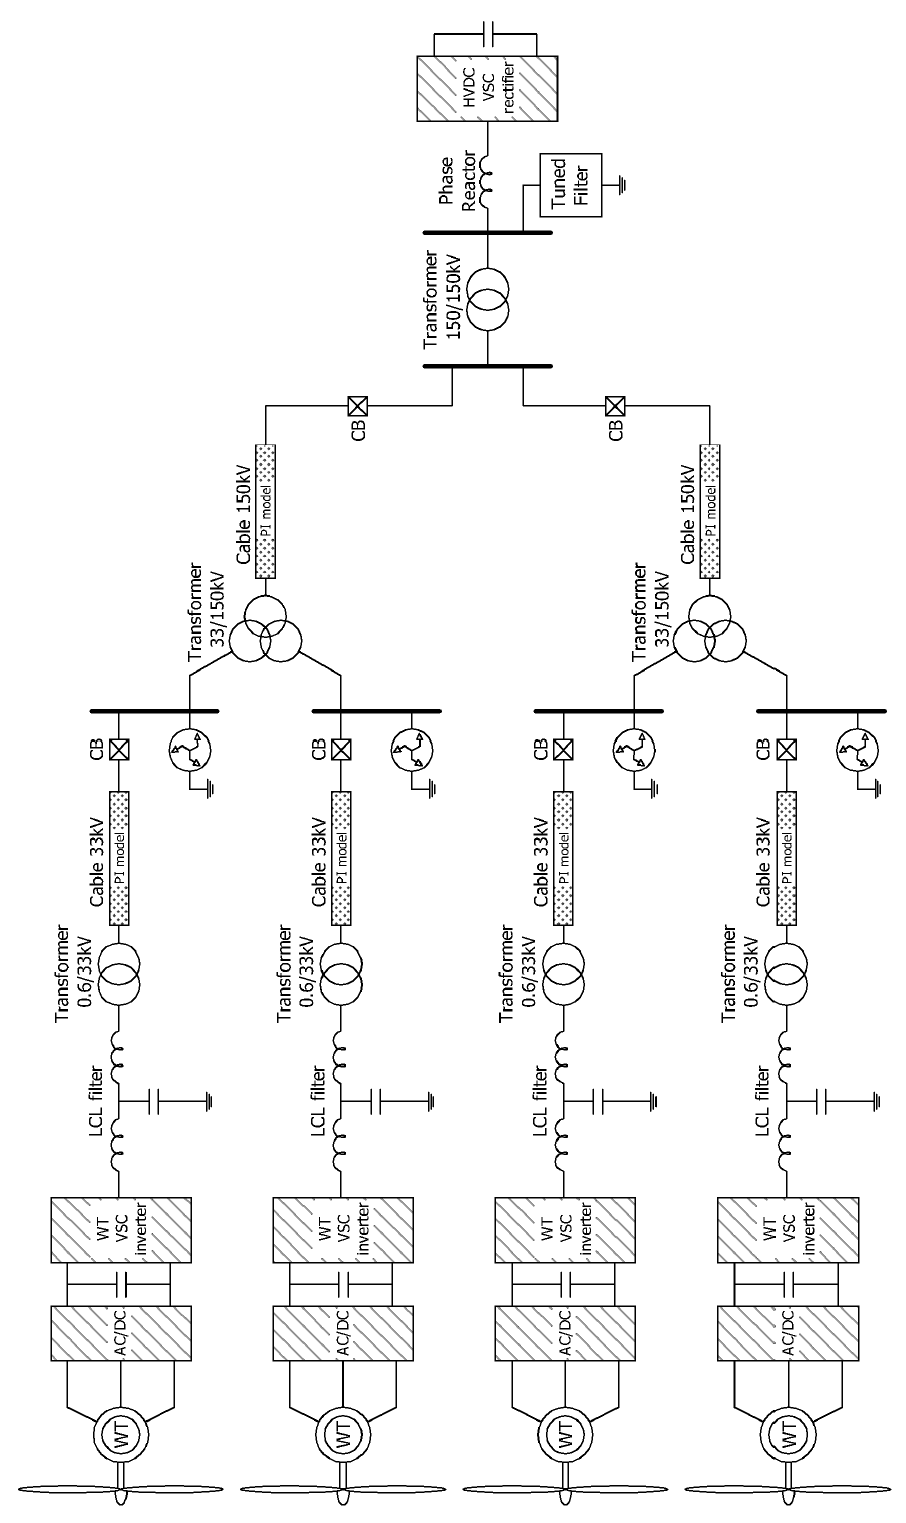
\includegraphics[width=0.9\textwidth]{img/system_full.png}
  	\caption{Considered 400MW Wind Power Plant}
  	\label{fig:systemfull}
\end{figure}
\FloatBarrier

Each of four branch is formed by ten 10-MW wind turbines with a terminal voltage of 690V. The aggregated model of each branch is used where each set of ten turbines is lumped and modelled as a single aggregated turbine, represented by a 100 MW turbine. Each aggregated turbine is connected to the LCL filter. Behind the LCL filter there are elements of collection grid: 690V/33kV transformer and an 8km underground collector cable (33kV). 33kV cable is linked to the 150kV transmission cable with a length of 58km via a 150kV/33kV/33kV three winding transformer with YN-dd configuration. The 150kV transmission cable is tied to the VSC-HVDC rectifier through a 150kV/150kV transformer and a phase reactor with an tuned shunt capacitor filter.

\subsection{Network impedance model}
Equivalent impedance diagram of WPP AC system is shown in the Figure~\ref{fig:systemcase3}. All of the parameters are converted to the 150kV equivalent voltage level. Table~\ref{tab:systemdata} presents the values of parameters in the network. The impedances of VSC-WT inverters and VSC-HVDC rectifier are calculated on the basis of three different methods presented in Section~\ref{sec:powerconverters}. The resulting impedances are presented in Section~\ref{sec:convertersmodels}.

\begin{figure}[htb]
	\centering
	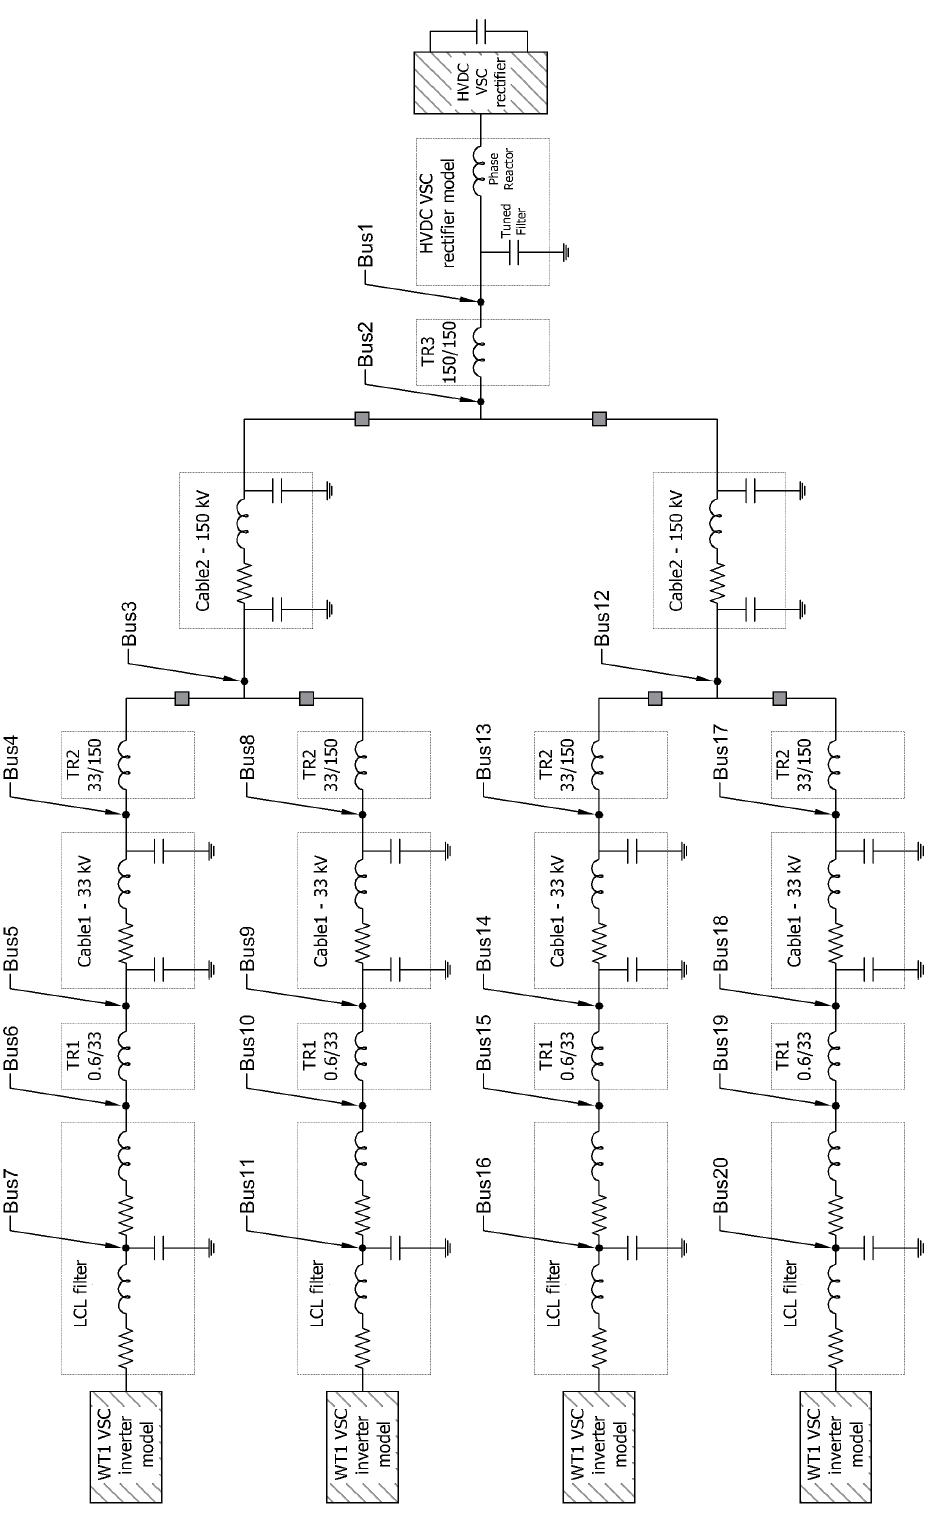
\includegraphics[width=0.9\textwidth]{img/Case3/system_case3.png}
  	\caption{Impedance diagram of the WPP network.}
  	\label{fig:systemcase3}
\end{figure}
\FloatBarrier

\begin{table}[htb]
	\centering
	\caption{Basic data of the system element at the equivalent voltage level of 150 kV.}
	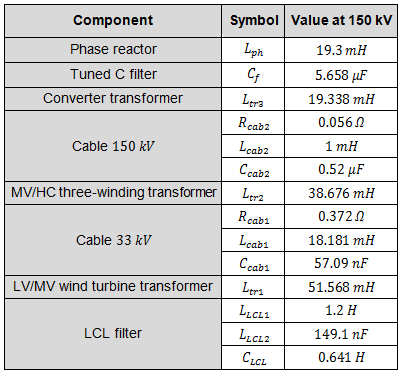
\includegraphics[width=0.5\textwidth]{img/table_systemdata.png}
  	\label{tab:systemdata}
\end{table}
\FloatBarrier



\begin{comment}
\floatsetup[table]{capposition=top}
\setlength{\arrayrulewidth}{0.2mm} %% border width
\arrayrulecolor[HTML]{000000} %% border color
\setlength{\tabcolsep}{6pt} %% separator of granic kolumn
\renewcommand{\arraystretch}{1} %% pionowe odstepy
\newcolumntype{d}{>{\columncolor{lightgray}} p{5cm}} %% ustawienia dla kolumny typu "d"
%\cellcolor[HTML]{AA0044} AND    \\
%\rowcolor{lightgray} \multicolumn{3}{|c|}{Country List} \\
%\rowcolor{gray}
\begin{table}
\centering
\begin{tabular}{ |d| p{3cm} | p{3cm} |  }
\hline
\rowcolor{lightgray} \textbf{\Large{Component}} & Symbol & Value at 150kV \\[3ex]
\hline
Phase reactor & $L_{ph}$ & $19.3 mH$ \\ \hline
Tuned C filter & $C_f$ & $5.658e-6 F$ \\ \hline
Converter transformer & $L_tr3$ & $19.338mH$ \\ \hline
Cable 150kV & $R_cab2$ & $0.056\Omega$ \\
 	& $L_cab2$ & $1mH$ \\
	& $C_cab2$ & $0.52e-6F$ \\ \hline
MV/HV three-winding transformer & $L_tr2$ & $0.372\Omega$ \\ \hline
Cable 33kV & $R_cab1$ & $0.372\Omega$ \\
	& $L_cab1$ & $18.181mH$ \\
	& $C_cab1$ & $5.709e-8F$ \\ \hline
LV/MV WT transformer & $L_tr1$ & $51.568mH$ \\ \hline
LCL filter & $L_LCL^1$ & $1.2H$ \\
	& $L_LCL^2$ & $1.491e-7F$ \\
	& $C_LCL$ & $0.641H$ \\ \hline
\end{tabular}
\caption{System data.}
\label{tab:systemdata}
\end{table}
\FloatBarrier

Tuned C filter $C_f$
Converter transformer $L_tr3$
Cable 150kV $R_cab2$
$L_cab2$
$C_cab2$
MV/HV transformer $L_tr2$
Cable 33kV $R_cab1$
$L_cab1$
$C_cab1$
LV/MV transformer $L_tr1$
LCL filter$L_LCL^1$
$L_LCL^2$
$C_LCL$
\end{comment}



\subsection{Topology cases} \label{sec:topologycases}
In the study, we approach comparison between different topologies. There are three topology cases examined. In principle, the difference between three topology depends on the number of included branches with aggregated wind turbines (1, 2 or 4 branches). The buses in the figures have assigned numbers which we employ in further analysis.
\begin{itemize}
	\item Case 1 model consist of one aggregated WT. In this case only one out of four branches is connected. The other three branches are disconnected by circuit breakers at the lower side of the three-winding transformers. Both branches connected to the lower other 150kV cable are disconnected, therefore this line is also disconnected. The topology of this system is presented in the Figure~\ref{fig:systemcase1}. 
	
\begin{figure}[htb]
	\centering
	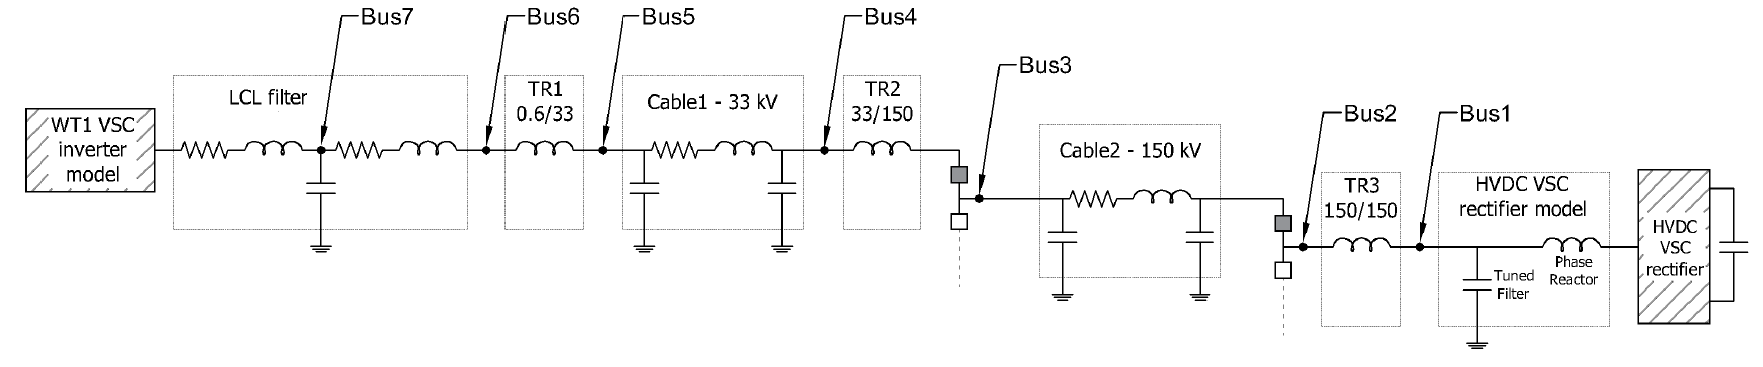
\includegraphics[width=1\textwidth]{img/Case1/system_case1.png}
  	\caption{Case 1 impedance diagram.}
  	\label{fig:systemcase1}
\end{figure}
\FloatBarrier

\item Case 2 includes one more aggregated turbine branch than Case 1. The second WT branch is connected to the first three-winding transformer. The second 150kV line is still disconnected. The topology of this system is presented in the Figure~\ref{fig:systemcase2}.

\begin{figure}[htb]
	\centering
	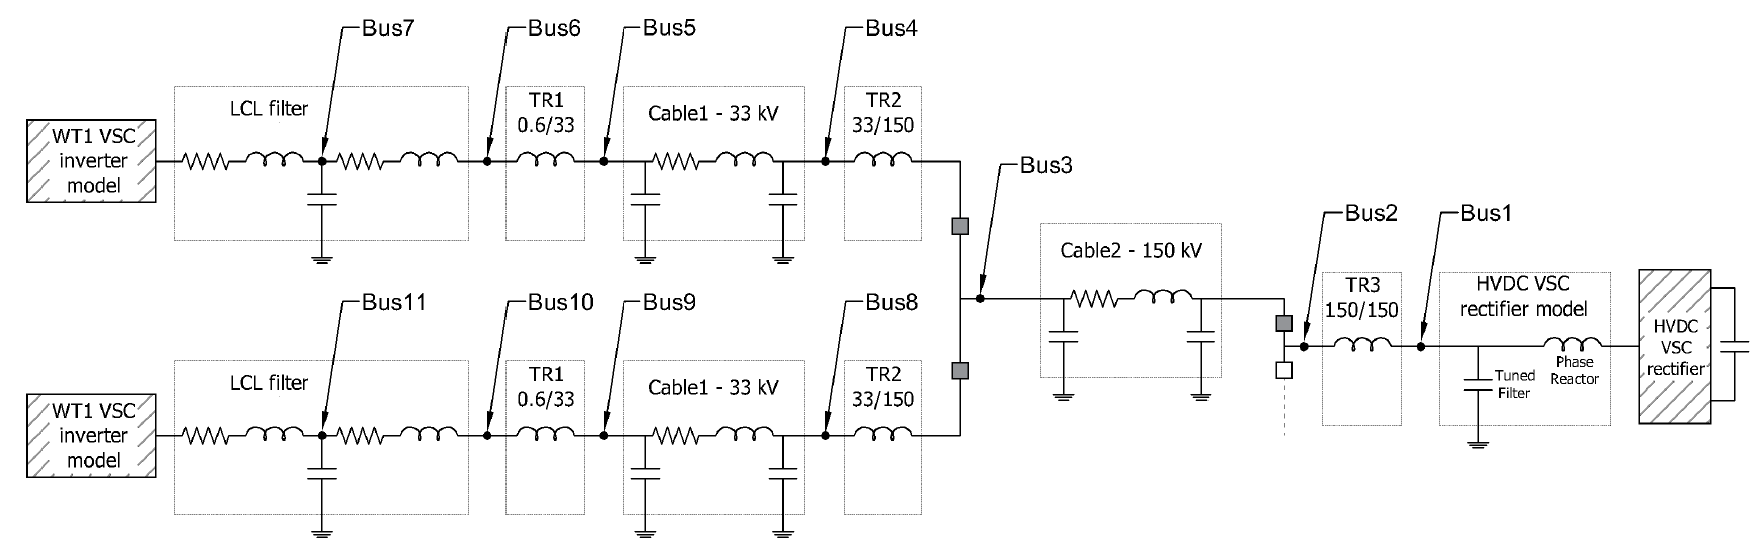
\includegraphics[width=1\textwidth]{img/Case2/system_case2.png}
  	\caption{Case 2 impedance diagram.}
  	\label{fig:systemcase2}
\end{figure}
\FloatBarrier

\item Case 3 consists of all elements in the networks. All branches are activated, therefore all elements are included in analysis. This topology is presented in the previous section, in the Figure~\ref{fig:systemcase3}.
\end{itemize}

\subsection{Power converters models} \label{sec:convertersmodels}
All of the elements excluding converters are modelled as the RLC elements. The principles of modelling of the elements are described in Section~\ref{sec:modellingofelements}. This section explains also the three different approaches to model converters (Section~\ref{sec:powerconverters}). In whole Chapter II of the thesis containing results of simulation, for simplicity, we refer to the different models of converters as follows: $VS$ – the model where both WT and HVDC converters are modelled as voltage sources (Section~\ref{sec:powerconverters-vscs}), $CS-WT$ or $CS$ – where WT converter is modelled as a current source and HVDC converter is still represented by voltage source (Section~\ref{sec:powerconverters-vscs}), $Z(s)$ – where both converters are represented by non-linear impedance models (Section~\ref{sec:powerconverters-zs}). 

Following tables (Table~\ref{tab:wttable} and Table~\ref{tab:hvdctable}) present the values of parameters which are implemented to the models described by equations (\ref{eq:impedance_wt}) and (\ref{eq:impedance_hvdc}). The values of these parameters are obtained from \cite{liusun2014}, however we rescale the resulting impedance into the 150kV equivalent circuit level. These changes are vital in order to align the impedance to further analysis where we combine the converter models with the other elements of the network. The values of other network elements are also at the equivalent 150kV voltage level (Table~\ref{tab:systemdata}).

\begin{table}[htb]
	\centering
	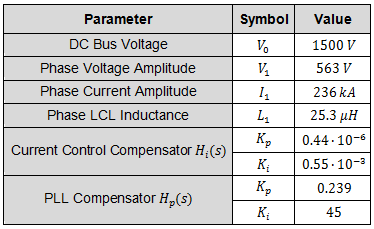
\includegraphics[width=0.5\textwidth]{img/tableWT.png}
  	\caption{WT converter nonlinear impedance model data.}
  	\label{tab:wttable}
\end{table}
\FloatBarrier

\begin{table}[htb]
	\centering
	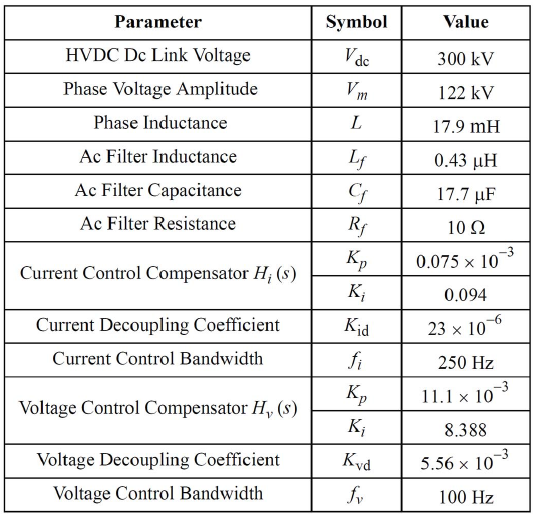
\includegraphics[width=0.5\textwidth]{img/tableHVDC.png}
  	\caption{HVDC converter nonlinear impedance model data.}
  	\label{tab:hvdctable}
\end{table}
\FloatBarrier

The results of impedance for both Z(s) modek converters are demonstrated in the Figure~\ref{fig:wtmodel} for WT-converter and in the Figure~\ref{fig:hvdcmodel} for HVDC converter. Both plots include curves of impedance magnitude and impedance angle for positive-sequence and negative-sequence in the domain of frequency.

\begin{figure}[htb]
	\centering
	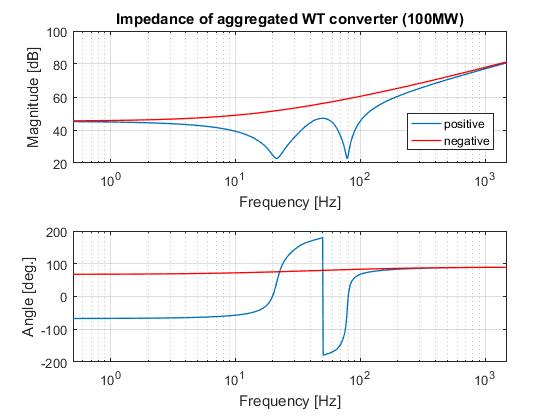
\includegraphics[width=0.8\textwidth]{img/modelWT.png}
  	\caption{WT converter nonlinear impedance model.}
  	\label{fig:wtmodel}
\end{figure}

\FloatBarrier
\begin{figure}[htb]
	\centering
	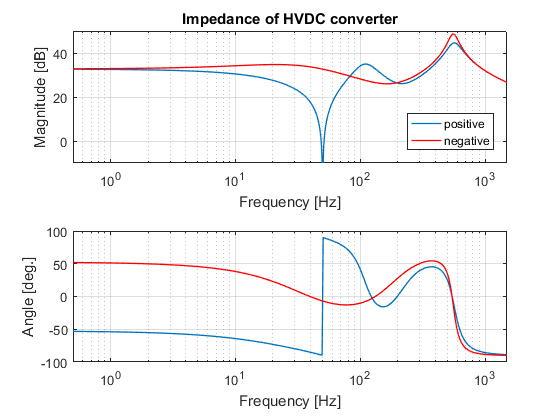
\includegraphics[width=0.8\textwidth]{img/modelHVDC.png}
  	\caption{HVDC converter nonlinear impedance model.}
  	\label{fig:hvdcmodel}
\end{figure}
\FloatBarrier

For both converters, we note sharp changes in the values of positive-sequence impedance angle at the fundamental frequency. On the other hand, the values of magnitudes and angles of negative-sequence are quite smooth for both converters. Moreover, we observe that above approximately second frequency order the curves of positive- and negative-sequences are very close to each other for all four plots.

Having in mind the different voltage level, thus different values of impedance, the outcome obtained correspond to the results from \cite{liusun2014}.

\section{Comparison of resonance frequencies between different topology cases and converter models} \label{sec:comparison1}
The first objective of this section is to compare results of resonance frequencies for three topology cases (Section~\ref{sec:topologycases}) in utilizing different converter models: VS, CS and Z(s). The description of modelling converter as VS, CS and Z(s) can be found in Section~\ref{sec:powerconverters}. The comparison is performed based on two methods: Frequency Sweep (Section~\ref{sec:theoryfs}) and Harmonic Resonance Modal Analysis (Section~\ref{sec:theoryhrma}). Secondly, on the basis of HRMA we spot the buses that have the most significant influence on the particular resonance frequencies. This identification is very useful for further study of implementation of filters, however filters are not investigated deeply in this study.

\subsection{Case 1}
\paragraph{Frequency Sweep}
Figure~\ref{fig:case1fslin} presents implementation of the frequency sweep method. All three converter models are included. The frequency sweep always refers to the particular node in the network. For this study, the bus number 7 (see Figure~\ref{fig:systemcase1}) is the bus of observation. In other words, the impedance is seen from that point of the network.

\begin{figure}[htb]
	\centering
	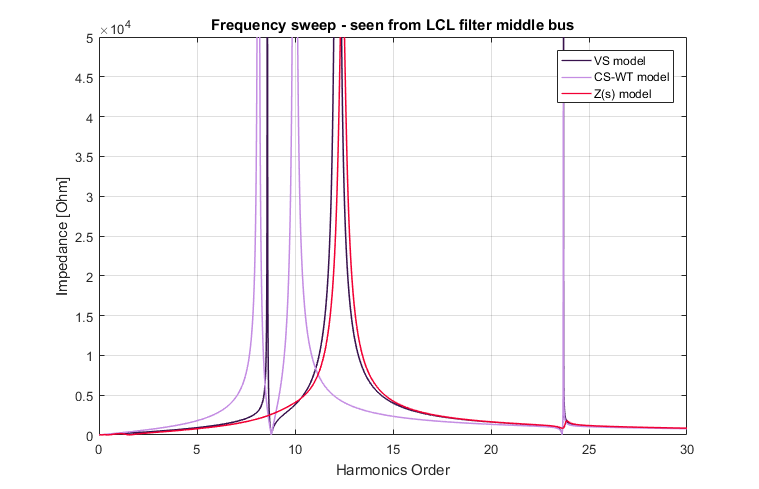
\includegraphics[width=1\textwidth]{img/Case1/Case1_FS_lin.png}
  	\caption{Impedance curves from FS - linear.}
  	\label{fig:case1fslin}
\end{figure}
\FloatBarrier

For easier analysis, the Figure~\ref{fig:case1fslog} presents the same data but with logarithmic vertical axis.

\begin{figure}[htb]
	\centering
	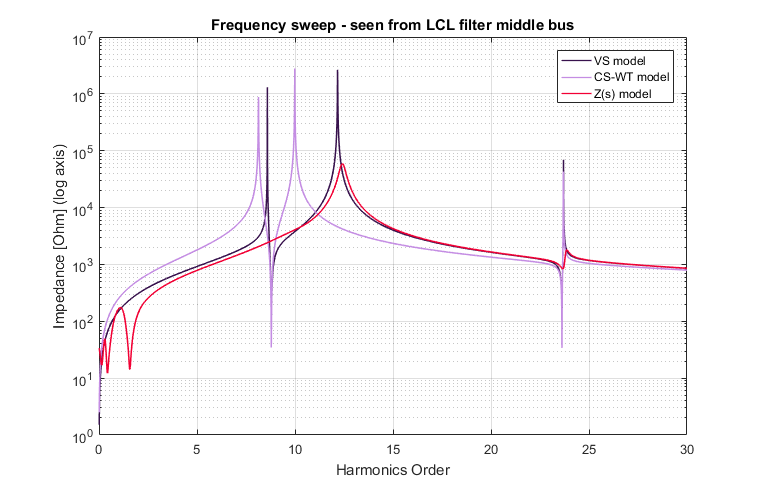
\includegraphics[width=1\textwidth]{img/Case1/Case1_FS_log.png}
  	\caption{Impedance curves from FS - log.}
  	\label{fig:case1fslog}
\end{figure}
\FloatBarrier

We can clearly see that the resonance frequencies alter for different models of converters. Table~\ref{tab:case1tablefs} presents  resonance frequencies values obtained from this analysis. The values of frequencies are identified in the points where the impedance curves reach local extreme values.

\begin{table}[htb]
	\centering
	\caption{Results of frequency sweep.}
	\includegraphics[width=0.5\textwidth]{img/Case1/table_FS.png}
  	\label{tab:case1tablefs}
\end{table}
\FloatBarrier

First of all, discover some peaking values of impedance for very low frequency orders (around fundamental frequency) in Z(s) model. These peaks are at much lower impedance level than the other values for higher orders. We exclude these peaks from our further analysis, reasoning that such a phenomenon needs more detailed research focused mainly on that problem and it won't be an issue in this study.

For VS model (within the examined frequency range) we observe three resonance frequencies. Similarly, in case of CS model – there are three resonance frequencies. For the Z(s) model of converters only two resonance frequencies are noted (as aforementioned, the low peaks around fundamental frequency are ignored).

Moreover, the values of impedance for Z(s) model are significantly reduced comparing to the VS and CS models. We can mark that the principles of modelling converters by this method leads to higher values of damping than by modelling as voltage or current source. The detailed description is provided in Section~\ref{sec:powerconverters-zs} and in \cite{liusun2013, liusun2014}.

\paragraph{Harmonic Resonance Modal Analysis}
In this section we compare the results of frequency sweep to the results of Harmonic Resonance Modal Analysis. As mentioned in Section \ref{sec:theoryhrma}, with HRMA method we also gain values of participation factors which suggest buses and elements which influence resonance more than others buses/elements. The Figures~\ref{fig:case1hrma1}, \ref{fig:case1hrma2} and \ref{fig:case1hrma3} present the curves of modal impedance in domain of harmonic order.

The Figure~\ref{fig:case1hrma1} illustrates the modal impedance for three models. Only maximum modal impedance for each frequency order is selected and plotted.

\begin{figure}[htb]
	\centering
	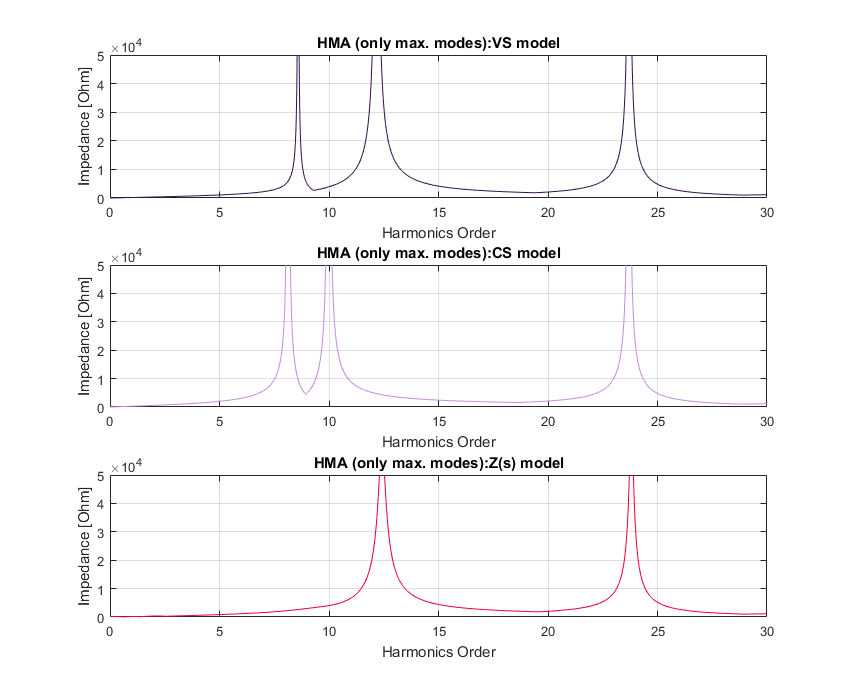
\includegraphics[width=1\textwidth]{img/Case1/Case1_HMA_max.png}
  	\caption{Case 1 - HRMA method. Maximum modal impedance curves.}
  	\label{fig:case1hrma1}
\end{figure}
\FloatBarrier

In the Figure~\ref{fig:case1hrma2}, we observe the very similar shapes of curves, however, this time all the modes are drawn. Most of the modes are barely visible since they equals zero or very small values for whole range of frequencies. 

\begin{figure}[htb]
	\centering
	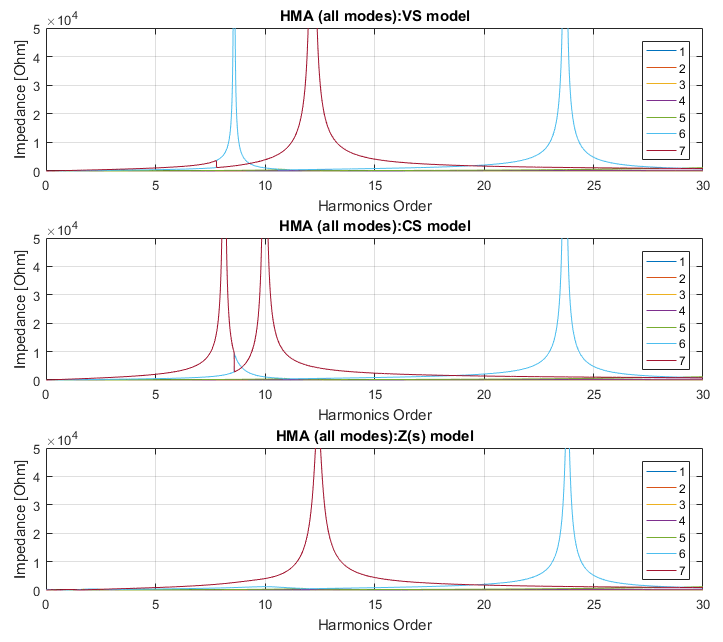
\includegraphics[width=1\textwidth]{img/Case1/Case1_HMA_all.png}
  	\caption{Case 1 - HRMA method. Impedance curves of all modes.}
  	\label{fig:case1hrma2}
\end{figure}
\FloatBarrier

The graphs above distinguish two modes which are peaking for all thre models - mode 6. and 7. Modal impedance for these modes reaches much higher value at the frequencies of resonance. The modes that determine the resonances are called critical modes. The critical modes impedances only, with full range of impedance, are plotted in the Figure~\ref{fig:case1hrma3}.

\begin{figure}[htb]
	\centering
	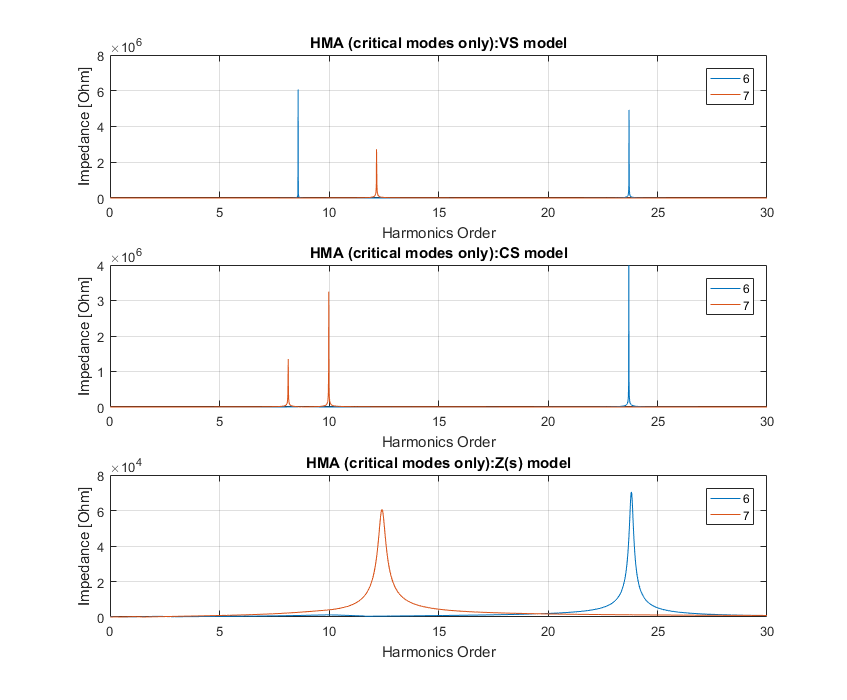
\includegraphics[width=1\textwidth]{img/Case1/Case1_HMA_crit.png}
  	\caption{Case 1 - HRMA method. Impedance curves of critical modes.}
  	\label{fig:case1hrma3}
\end{figure}
\FloatBarrier

As explained in Section~\ref{sec:theoryhrma}, even though the total number of modes equals the number of buses in the network, these modes do not correspond to the network buses exactly. Their correlation is reported by the participation factors presented in Table~\ref{tab:case1tablehrma2}. Before, Table~\ref{tab:case1tablehrma1} presents the critical modal impedance values and the harmonic orders for frequencies when the critical modal impedances occur.

\begin{table}[htb]
	\centering
	\caption{Case 1 - HRMA method results.}
	\label{tab:case1tablehrma1}
	\includegraphics[width=0.5\textwidth]{img/Case1/table_HRMA1.png}
\end{table}
\FloatBarrier

\begin{table}[htb]
	\caption{Case 1 - HRMA method results - PFs.}
	\label{tab:case1tablehrma2}
	\centering
	\includegraphics[width=1\textwidth]{img/Case1/table_HRMA2.png}
\end{table}
\FloatBarrier

The study of participation factors is very relevant for localization of the best nodes in a network for filter implementation. The participation factors express the significance of a bus in resonance emission. Therefore, the modification of capacitance/inductance at the point of the network with the highest participation factor should trigger to the most powerful change of the resonance frequency. The details about participation factors in Section~\ref{sec:theoryhrma} and \cite{xu2005}.

In the study of Case 1, from the values of participation factors, one can easily recognize that the buses number 5 and 7 are the two buses which contribute to the resonance frequencies more than the others. As we can see, these two buses play the lead role in all three different models what indirectly confirms the consistency of three approaches. We also observe only two resonant frequencies for Z(s) model. From the values of the participation factors, we also derive some conclusions. Since the two resonance frequencies from the first two models are mostly correlated to the bus 7 and similarly for the one of the resonance frequencies from the Z(s) model, the two resonance frequencies from VS and CS models could have been merged into one resonance frequency from Z(s) model. Otherwise, due to the higher resistance of the Z(s) model, one of the resonance frequency could have been smoothed down to the insignificant value.

\paragraph{DIgSILENT Power Factory model}
In this simulation, we use the Power Factory model presented in the Figure~\ref{fig:c1pfmodel}. The model is combined of basic RLC elements.

\begin{figure}[htb]
	\centering
	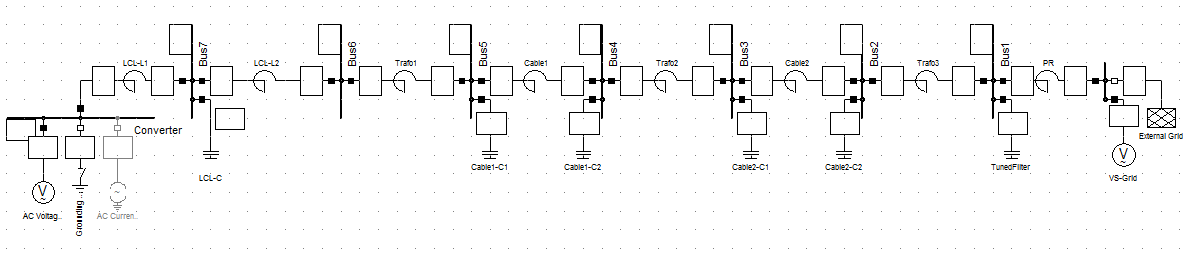
\includegraphics[width=1\textwidth]{img/Case1/PF_model.png}
  	\caption{Case 1 - Power Factory model.}
  	\label{fig:c1pfmodel}
\end{figure}
\FloatBarrier

Only two models: VS and CS-WT are simulated. We perform so-called \textit{Impedance Frequency Characteristic} calculation in the software. Figures~\ref{fig:c1pfvs1} and \ref{fig:c1pfcs1} show the results of frequency sweep for VS and CS-WT model, respectively.

\begin{figure}[htb]
	\centering
	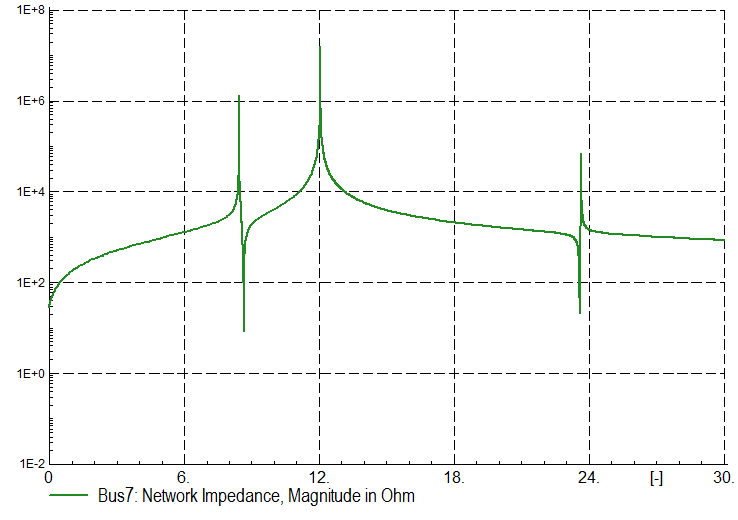
\includegraphics[width=0.8\textwidth]{img/Case1/PF_imp7_VS.PNG}
  	\caption{Case 1 - Power Factory VS model results}
  	\label{fig:c1pfvs1}
\end{figure}
\FloatBarrier

\begin{figure}[htb]
	\centering
	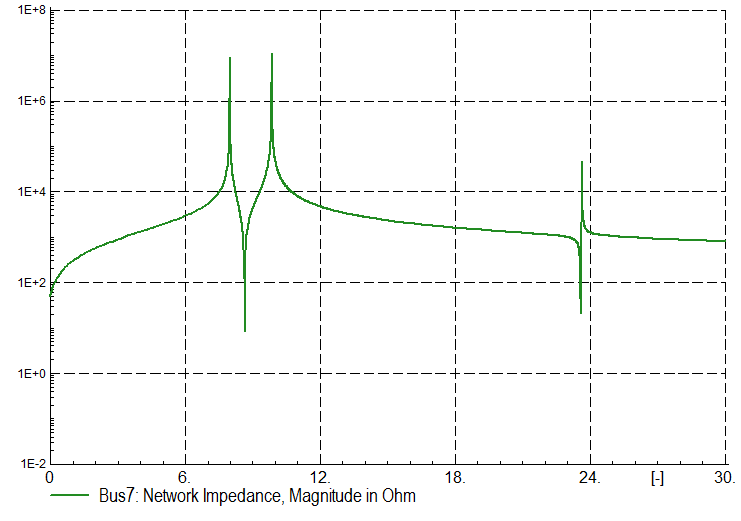
\includegraphics[width=0.8\textwidth]{img/Case1/PF_imp7_CS.PNG}
  	\caption{Case 1 - Power Factory CS model results}
  	\label{fig:c1pfcs1}
\end{figure}
\FloatBarrier

We can examine the figures obtained from the Power Factory software and conclude that, regarding resonant frequency values, they are definitely coincident with the ones received from detail analysis in MATLAB. However, the peak values of impedances are different. The differences probably source in the settings of \textit{Impedance Calculation} for frequency sweep analysis. The step size of the simulation was set to the value of 0.1 Hz; furthermore the \textit{Automatic Step Size Adaptation} was selected. Hence, difference in the values of impedance occurs. The dependence of the peak values from the value of step size was checked through similar simulation with different step sizes. The observation confirms that the step size influences peak impedance values.

What is more important in this study are the values of the resonance frequencies. The values obtained by Power Factory confirms the values gained from MATLAB analysis of both frequency sweep and modal analysis.

\begin{table}[htb]
	\centering
	\caption{Case 1 - Power Factory frequency results.}
	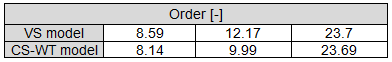
\includegraphics[width=0.6\textwidth]{img/Case1/table_powerfactory.PNG}
  	\label{tab:c1pftable}
\end{table}
\FloatBarrier

As aforementioned, the observation of network impedance (frequency sweep) is performed from the specified bus in the network (bus 7). Due to the Power Factory software, we can performed the observation of impedance from each of the bus in the considered case. The results of frequency sweep seen from all 7 buses is presented in the Figure~\ref{fig:c1pfvs2} and \ref{fig:c1pfcs2}, for VS model and CS model, respectively.

\begin{figure}[htb]
	\centering
	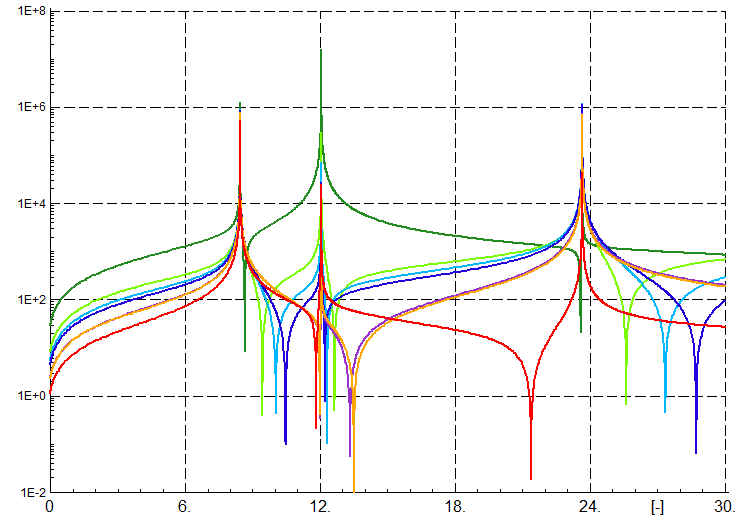
\includegraphics[width=0.8\textwidth]{img/Case1/PF_impAll_VS.PNG}
	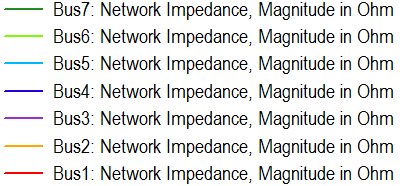
\includegraphics[width=0.4\textwidth]{img/Case1/PF_impAllLegend.PNG}
	\caption{Case 1 VS - all buses - Power Factory resonance results.}
  	\label{fig:c1pfvs2}
\end{figure}
\FloatBarrier

\begin{figure}[htb]
	\centering
	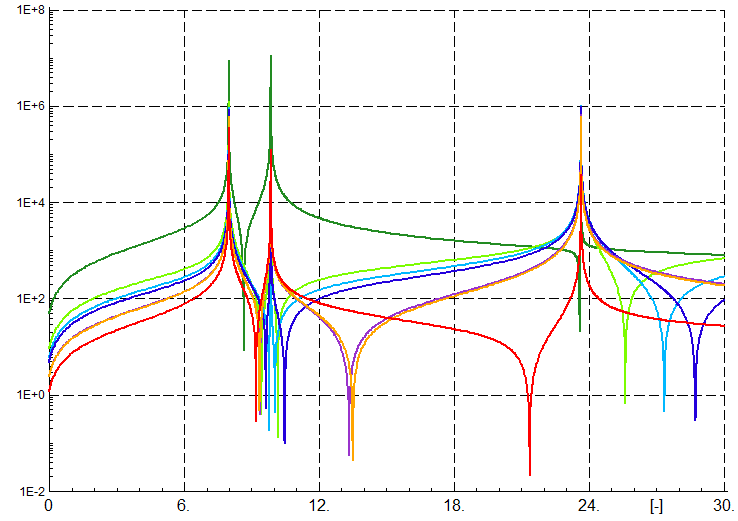
\includegraphics[width=0.8\textwidth]{img/Case1/PF_impAll_CS.PNG}
	%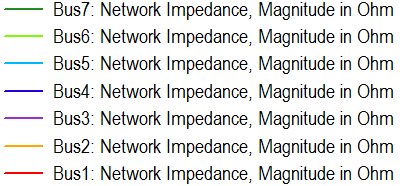
\includegraphics[width=0.3\textwidth]{img/Case1/PF_impAllLegend.PNG}
	\caption{Case 1 CS - all buses - Power Factory resonance results.}
  	\label{fig:c1pfcs2}
\end{figure}
\FloatBarrier

The examination of the curves above demonstrates that the peaking impedances for both models occur at the same frequencies, regardless the bus of observation. On the other hand, the dips of impedance undoubtedly depend on the bus where the observation is performed from. Coupling with the principles of parallel and series resonance, we can draw the two conclusions. Firstly, the series resonance frequency depends on the bus in the network i.e. series resonance frequency is different at the different points in the network. Secondly, since the peaks of the impedance, so the parallel resonance frequencies, are the same regardless the bus of observation, we conclude that the parallel resonance frequencies do not depend on the point of observation. The confirmation of the latter statement we recognize in the HRMA method. As described in Section~\ref{sec:theoryhrma}, the method is utilized in order to investigate the parallel resonance and is not performed for particular bus, but for entire network. The frequencies collected from that method are exactly the frequencies obtained for every different case of observation bus in the frequency sweep method.

\paragraph{FS and HRMA results comparison}
In the three previous paragraphs the results of frequency sweep analysis, harmonic resonance modal analysis, both performed in MATLAB were presented. Moreover, these results we couple with frequency sweep tool in Power Factory software. The values of resonance frequencies obtained ambiguously confirms the correspondence of these three approaches to each other. The values of parallel resonant frequencies are the same for the considered accuracy.

The difference of the impedance peak values are not considered very deeply in this study. However, as aforementioned, these values very often depends on the step size of the calculation. Moreover, the threshold impedance values above which the impedance level is defined as dangerous should be assigned individually for each particular case of a network. Furthermore, the values of modal impedance from HRMA method does not exactly correspond to the real impedance value and should not be compared directly to the values of impedances obtained from frequency sweep or Power Factory tool.

\subsection{Case 2}
The topology Case 2 was presented in Section~\ref{sec:topologycases}. In this case, the Wind Power Plant consists of two branches. There is one aggregated Wind Turbine in each branch. The total power of connected Wind Turbines is 200 MW.

\paragraph{Frequency Sweep}
In the Figures~\ref{fig:case2fslin} and \ref{fig:case2fslog} the results of frequency sweep method are presented with linear and logarithmic impedance scale, respectively. Again, all three models of converters are included. The impedance of the grid is seen again from the bus number 7 i.e. middle bus of LCL filter in the first branch. Since the branch 1 is the same the branch 2, we could collect the same curves for impedance observed from bus 11.

\begin{figure}[htb]
	\centering
	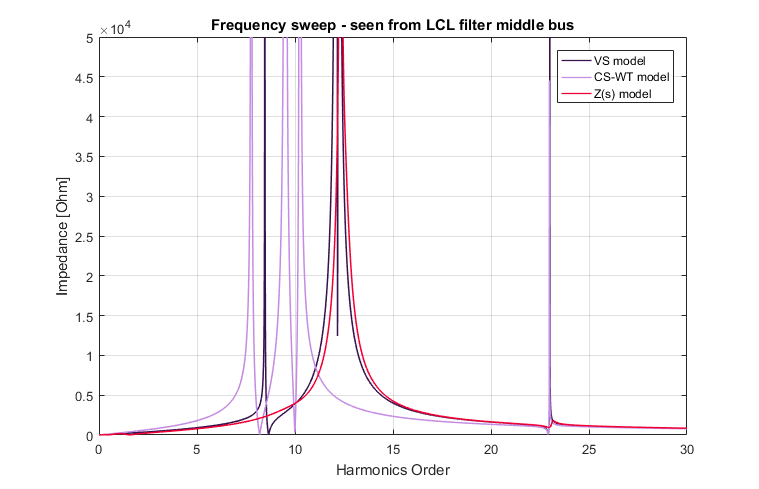
\includegraphics[width=1\textwidth]{img/Case2/Case2_FS_lin.png}
  	\caption{case 2 Impedance curves from FS - linear.}
  	\label{fig:case2fslin}
\end{figure}
\FloatBarrier

\begin{figure}[htb]
	\centering
	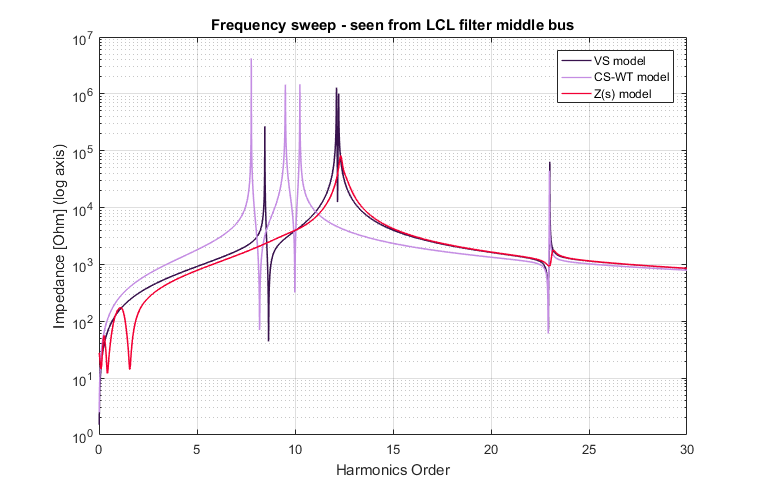
\includegraphics[width=1\textwidth]{img/Case2/Case2_FS_log.png}
  	\caption{case 2 Impedance curves from FS - log.}
  	\label{fig:case2fslog}
\end{figure}
\FloatBarrier

Table~\ref{tab:case2tablefs} presents resonance frequencies values from the graphs above. The values of frequencies are identified when impedance reaches local extreme values (parallel resonance). This time again, the results of resonance frequencies around fundamental value are ignored.

\begin{table}[htb]
	\centering
	\caption{Case 2 FS results.}
	\label{tab:case2tablefs}
	\includegraphics[width=0.5\textwidth]{img/Case2/table_FS.png}
\end{table}
\FloatBarrier

We can note that undoubtedly this time there are four resonant frequencies for Current Source model. The curve of VS model consists surely of three peaks, however, looking at the values, the fourth one is very close to the other around $12^{th}$ order. Therefore, it is harder to notice it from the graph. The Z(s) model comprises two impedance rises, excluding ones around fundamental frequency. The value of impedance of Z(s) model is significantly lower than in other models, similarly to the Case 1. We carry on further conclusions and contemplations about the resonant frequencies after presenting HRMA results for this case.

\paragraph{Harmonic Resonance Modal Analysis}
The Figures~\ref{fig:case2hrma1}-\ref{fig:case2hrma3} illustrate the HRMA result curves. Similarly to the previous topology case, the following graphs shows the curves of maximum modal impedances for each harmonic order, than modal impedances with respect to the each mode separately and finally, critical modes only i.e. the modes that are assigned to the modal impedance peaks.

\begin{figure}[htb]
	\centering
	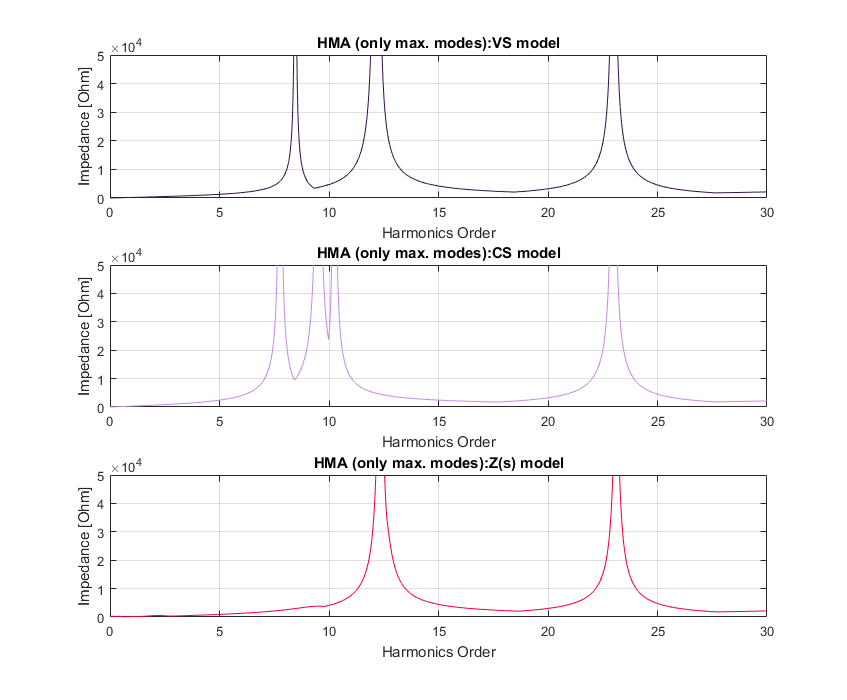
\includegraphics[width=1\textwidth]{img/Case2/Case2_HMA_max.png}
  	\caption{Case 2 - HRMA method. Maximum modal impedance curves.}
  	\label{fig:case2hrma1}
\end{figure}
\FloatBarrier

\begin{figure}[htb]
	\centering
	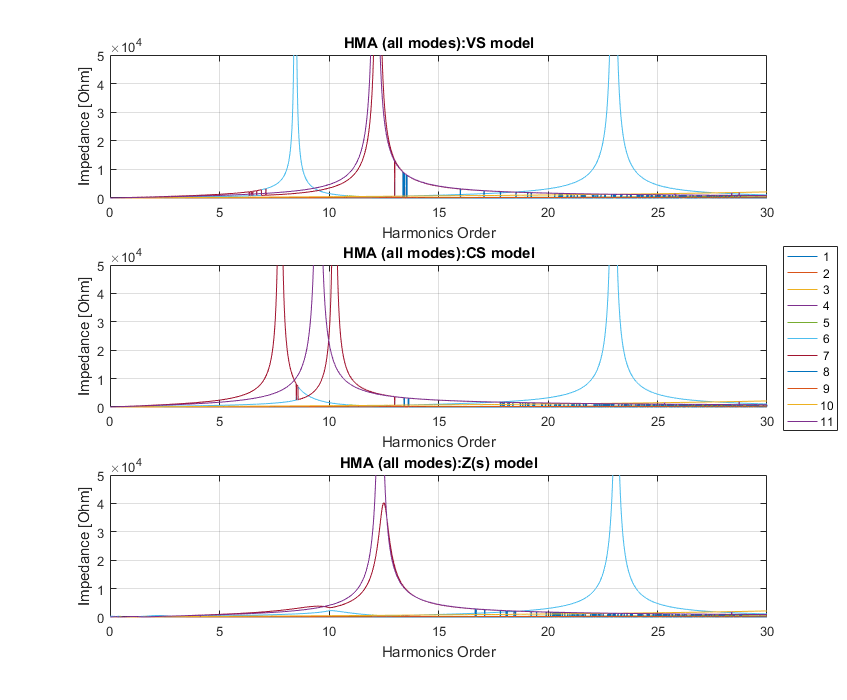
\includegraphics[width=1\textwidth]{img/Case2/Case2_HMA_all.png}
  	\caption{Case 2 - HRMA method. Impedance curves of all modes.}
  	\label{fig:case2hrma2}
\end{figure}
\FloatBarrier

\begin{figure}[htb]
	\centering
	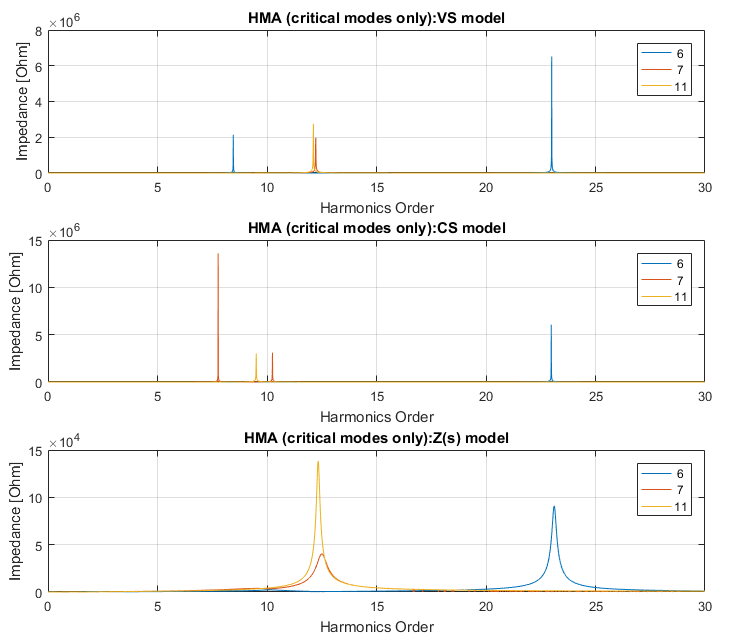
\includegraphics[width=1\textwidth]{img/Case2/Case2_HMA_crit.png}
  	\caption{Case 2 - HRMA method. Impedance curves of critical modes.}
  	\label{fig:case2hrma3}
\end{figure}
\FloatBarrier

Again, the participation factors point out the connotation of each mode to the real buses in the network. Table~\ref{tab:case2tablehrma2} presents the participation factors for the detected resonant frequencies i.e. frequencies at which the modal impedance rises occur. The values of critical impedances and critical modes for each of them are gathered in Table~\ref{tab:case2tablehrma1}.

\begin{table}[htb]
	\centering
	\caption{Case 2 - HRMA method results.}
	\label{tab:case2tablehrma1}
	\includegraphics[width=0.45\textwidth]{img/Case2/table_HRMA1.png}
\end{table}
\FloatBarrier

\begin{table}[htb]
	\caption{Case 2 - HRMA method results - PFs.}
	\label{tab:case2tablehrma2}
	\centering
	\includegraphics[width=0.9\textwidth]{img/Case2/table_HRMA2.png}
\end{table}
\FloatBarrier

This time we observe one significant difference between the frequency sweep curves and HRMA curves. For Z(s) model, one of the frequency that is missing in the frequency sweep method appears in the HRMA curves. To interpret this we look at the value of the modal impedance for this resonant frequency or at the figures. The value of critical impedance of critical module is much smaller than the other modal critical impedances (for other resonant frequencies). Since the resonant frequencies are recognized as the extreme points of impedance curves, peak value are identified in this way. However, in order to exclude this frequency from the results, further investigation of for example minimum dangerous impedance would be necessary.

Besides this difference, the results of frequencies converge completely. 

From the values of participation factors we derive couple of conclusions. First of all, the values of participation factors for buses of branch 1 (4-7) correspond to the buses of branch 2 (8-11) with the same values. It shows that from the modal analysis point of view the wind turbine branches are the same and the participation factor is distributed symmetrically to the two analogical buses of both branches. Secondly, comparing the results of participation factors for Case 1 and Case 2 we can observe some similarities in apparition of the new resonant frequency. For both VS and CS-WT model, the lowest resonant frequency stays approximately at the same level, to be more precise is slightly shifted down to the lower value. The value of participation factor is divided equally into two analogical buses. The second frequency from Case 1 seems to appear in Case 2 as two resonant frequencies, one greater and the other less than the frequency from Case 1. The values of participation factors for both cases for these frequencies appear to confirm this assumption since their values are again distributed equally and the values are very similar for the new two frequencies.

On the contrary, in the Z(s) model, the two frequencies stay at approximately the same level and the new resonance frequency appears \textit{independently} after adding new branch. As stated before, the value of critical impedance is very low.

From the curves of modal impedances with regards to each single node (Figure~\ref{fig:case2hrma2}), we observe that for resonance around $12^{th}$ order, the values of two modes are at the similar level of modal impedance for this value of resonance – mode 7 and mode 11. This condition disturbs the assumption settled in Section~\ref{sec:theoryhrma} and \cite{xu2005} that only one within the modal impedances is much greater than the others. As the result, we obtain inaccurate participation factors which do not sum to value around 1. For the new frequency, the sum of participation factors reaches 1.533 therefore all participation factors are is considered as inaccurate.

\paragraph{DIgSILENT Power Factory model}
Furthermore, the results of FS and HRMA are compared with the curves acquired from Power Factory software. Figure~\ref{fig:c2pfmodel} presents the diagram of the network used for calculation.

\begin{figure}[htb]
	\centering
	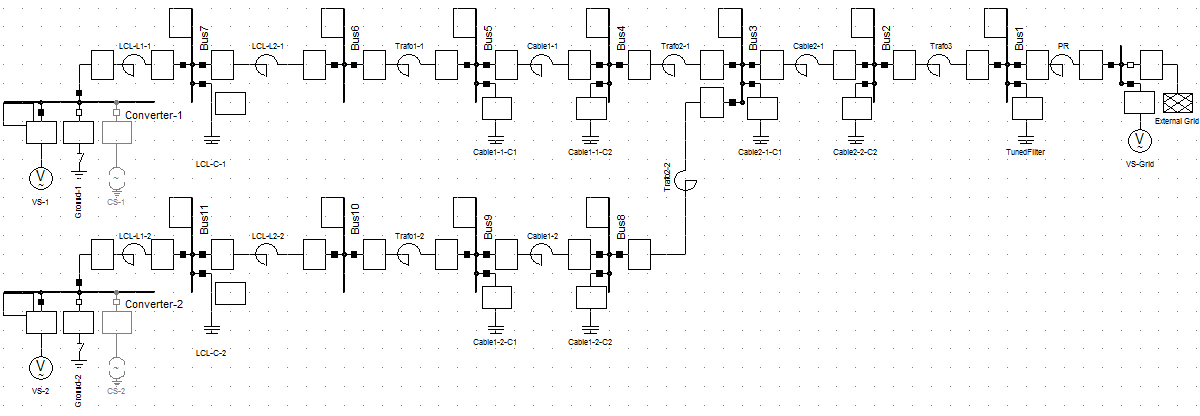
\includegraphics[width=1\textwidth]{img/Case2/PF_model.png}
  	\caption{Case 2 - Power Factory model.}
  	\label{fig:c2pfmodel}
\end{figure}
\FloatBarrier

Again, the models of VS and CS-WT are simulated for \textit{Impedance Frequency Characteristic} calculations. Figures~\ref{fig:c2pfvs1} and \ref{fig:c2pfcs1} present the results of frequency sweep for VS and CS-WT models, seen from the middle LCL filter bus i.e. the same bus as for MATLAB model – bus 7.

\begin{figure}[htb]
	\centering
	\includegraphics[width=0.8\textwidth]{img/Case2/PF_imp7_VS.PNG}
  	\caption{Case 2 - Power Factory VS model results}
  	\label{fig:c2pfvs1}
\end{figure}
\FloatBarrier

\begin{figure}[htb]
	\centering
	\includegraphics[width=0.8\textwidth]{img/Case2/PF_imp7_CS.PNG}
  	\caption{Case 2 - Power Factory CS model results}
  	\label{fig:c2pfcs1}
\end{figure}
\FloatBarrier

The resonant frequencies for peak impedances are measured by the software tool and presented in the Table~\ref{tab:c2pftable}.

\begin{table}[htb]
	\centering
	\caption{Case 2 - Power Factory frequency results.}
	\includegraphics[width=0.6\textwidth]{img/Case2/table_powerfactory.PNG}
  	\label{tab:c2pftable}
\end{table}
\FloatBarrier

The values of resonant frequencies are consistent with the values obtained both in FS and HRMA in MATLAB. Again, we present the impedance curves seen from other buses. The buses where the impedance is observed are buses 1-7. Since the two branches with wind turbines are the same, we know that the impedance curves seen from buses 4-7 are the same as seen from respective buses 8-11. Therefore the impedance curves for only one branch are sufficient. The Figure~\ref{fig:c2pfvs2} shows the curves for buses 1-7 for the VS model, while the Figure~\ref{fig:c2pfcs2} illustrate the same curves but for model CS-WT.

\begin{figure}[htb]
	\centering
	\includegraphics[width=0.8\textwidth]{img/Case2/PF_impAll_VS.PNG}
	\includegraphics[width=0.4\textwidth]{img/Case2/PF_impAllLegend.PNG}
	\caption{Case 2 VS - all buses - Power Factory resonance results.}
  	\label{fig:c2pfvs2}
\end{figure}
\FloatBarrier

\begin{figure}[htb]
	\centering
	\includegraphics[width=0.8\textwidth]{img/Case2/PF_impAll_CS.PNG}
	%\includegraphics[width=0.5\textwidth]{img/Case2/PF_impAllLegend.PNG}
	\caption{Case 2 CS - all buses - Power Factory resonance results.}
  	\label{fig:c2pfcs2}
\end{figure}
\FloatBarrier

The shapes of the curves indicate the same conclusions like for Case 1 i.e. the series and parallel resonance does depend on and does not depend on the point in the network, respectively. The previous section presenting results of Case 1 describes these principles in details.

\paragraph{Results comparison}
Similarly to the first case, the results of FS, HRMA and from Power Factory are very similar. For the considered accuracy, the values of corresponding frequencies are exactly the same. The important fact to highlight is that we obtain one resonance frequency more for HRMA comparing to FS in the Z(s) model. Even though the value of modal impedance is quite low comparing to the other resonance points, the level of impedance dangerous for the network is not identified and could apparently be already dangerous for the network. The situation suggests the conclusion that we should always consider both methods together and compare their outputs. Since the amount of data necessary for both methods is very similar, this does not pose a problem during analysis.

\subsection{Case 3}
The last topology case is described in Section~\ref{sec:topologycases}. All installed power (400 MW) and all elements of Wind Power Plant are considered.

\paragraph{Frequency Sweep}
Figures~\ref{fig:case3fslin} and \ref{fig:case3fslog} present the frequency sweep curves for linear and logarithmic scales, respectively. All three models are included. The bus of observation is again bus 7. All four wind turbine branches are equal therefore the features of those branches are symmetrical to each other. The groups of equal bus numbers at the wind turbine branches are: (4, 8, 13, 17), (5, 9, 14, 18), (6, 10, 15, 19), (7, 11, 16, 20). Moreover bus 3 and bus 12 are also symmetrical, installed at the end of two symmetrical cables connecting pairs of wind turbine branches.

\begin{figure}[htb]
	\centering
	\includegraphics[width=1\textwidth]{img/Case3/Case3_FS_lin.png}
  	\caption{case 3 Impedance curves from FS - linear.}
  	\label{fig:case3fslin}
\end{figure}
\FloatBarrier

\begin{figure}[htb]
	\centering
	\includegraphics[width=1\textwidth]{img/Case3/Case3_FS_log.png}
  	\caption{case 3 Impedance curves from FS - log.}
  	\label{fig:case3fslog}
\end{figure}
\FloatBarrier

Table~\ref{tab:case3tablefs} presents resonance frequency values and the peak values of corresponding impedances. The values around the fundamental frequency for Z(s) model are ignored.

\begin{table}[htb]
	\centering
	\caption{case 3 FS results.}
	\label{tab:case3tablefs}
	\includegraphics[width=0.5\textwidth]{img/Case3/table_FS.png}
\end{table}
\FloatBarrier

We can observe one additional resonance frequency for each of the VS and CS-WT models comparing to Case 2. However, pair of frequencies for each model have very similar values therefore, from the figure, could be considered as the one resonant frequency. Further examination and comparison of the frequency sweep results for all considered topology cases is presented in Section~\ref{sec:comparisoncases}.

\paragraph{Harmonic Resonance Modal Analysis}
Following Figures~\ref{fig:case3hrma1}, \ref{fig:case3hrma2} and \ref{fig:case3hrma3} shows the HRMA results. Again, the graphs present maximum modal impedances, modal impedances curves for all modes separately and critical modes curves alone.

\begin{figure}[htb]
	\centering
	\includegraphics[width=0.9\textwidth]{img/Case3/Case3_HMA_max.png}
  	\caption{Case 3 - HRMA method. Maximum modal impedance curves.}
  	\label{fig:case3hrma1}
\end{figure}
\FloatBarrier

\begin{figure}[htb]
	\centering
	\includegraphics[width=0.9\textwidth]{img/Case3/Case3_HMA_all.png}
  	\caption{Case 3 - HRMA method. Impedance curves of all modes.}
  	\label{fig:case3hrma2}
\end{figure}
\FloatBarrier

\begin{figure}[htb]
	\centering
	\includegraphics[width=1\textwidth]{img/Case3/Case3_HMA_crit.png}
  	\caption{Case 3 - HRMA method. Impedance curves of critical modes.}
  	\label{fig:case3hrma3}
\end{figure}
\FloatBarrier

With these results in mind, the values of critical impedances and values of participation factors for Case 3 are presented for each resonance frequency in Table~\ref{tab:case3tablehrma1} and \ref{tab:case3tablehrma2}, respectively.

\begin{table}[htb]
	\centering
	\caption{Case 3 - HRMA method results.}
	\label{tab:case3tablehrma1}
	\includegraphics[width=0.5\textwidth]{img/Case3/table_HRMA1.png}
\end{table}
\FloatBarrier

\begin{table}[htb]
	\caption{Case 3 - HRMA method results - PFs.}
	\label{tab:case3tablehrma2}
	\centering
	\includegraphics[width=1\textwidth]{img/Case3/table_HRMA2.png}
\end{table}
\FloatBarrier

Similarly to the Case 2, for Z(s) model we obtain one more resonance frequency from HRMA comparing to frequency sweep. Besides this frequency, the values of equivalent ones are the same or very similar. Again, the modal impedance value of critical mode for new frequency is very low. 

Furthermore, the participation factors for new frequency are probably inaccurate since the sum of them for the new frequency exceeds unity. Finally, we note that the participation factors are not completely symmetrical in some cases. The symmetry remains between the pair of branches 1 and 2 or 3 and 4 (the pairs connected to the same three-winding transformer) but symmetry of participation factors between pair branches connected to different three-winding transformers fades away for some cases.

\paragraph{DIgSILENT Power Factory model}
Analogically, we compare the results of FS and HRMA with the curves from Power Factory model. The model used in this case is presented in the Figure~\ref{fig:c3pfmodel}.

\begin{figure}[htb]
	\centering
	\includegraphics[width=1\textwidth]{img/Case3/PF_model.png}
  	\caption{Case 3 - Power Factory model.}
  	\label{fig:c3pfmodel}
\end{figure}
\FloatBarrier

The models of VS and CS-WT are simulated for Impedance Frequency Characteristic calculations. Figures~\ref{fig:c3pfvs1} and Figures~\ref{fig:c3pfcs1} present the results of frequency sweep for VS and CS-WT model, seen from the middle LCL filter bus i.e. the same bus as for MATLAB model – bus 7.

\begin{figure}[htb]
	\centering
	\includegraphics[width=0.8\textwidth]{img/Case3/PF_imp7_VS.PNG}
  	\caption{Case 3 - Power Factory VS model results}
  	\label{fig:c3pfvs1}
\end{figure}
\FloatBarrier

\begin{figure}[htb]
	\centering
	\includegraphics[width=0.8\textwidth]{img/Case3/PF_imp7_CS.PNG}
  	\caption{Case 3 - Power Factory CS model results}
  	\label{fig:c3pfcs1}
\end{figure}
\FloatBarrier

The resonant frequencies for peak impedances are measured in the software tool and presented in the Table~\ref{tab:c3pftable}.

\begin{table}[htb]
	\centering
	\caption{Case 3 - Power Factory frequency results.}
	\includegraphics[width=0.8\textwidth]{img/Case3/table_powerfactory.PNG}
  	\label{tab:c3pftable}
\end{table}
\FloatBarrier

One more time, the values obtained from Power Factory converge with those we collected from frequency sweep analysis in MATLAB. Similarly to the Case 2 analysis, the Figures~\ref{fig:c3pfvs2} and \ref{fig:c3pfcs2} show the curves for buses 1-7 for the VS model and CS-WT model, respectively.

\begin{figure}[htb]
	\centering
	\includegraphics[width=0.8\textwidth]{img/Case3/PF_impAll_VS.PNG}
	\includegraphics[width=0.4\textwidth]{img/Case3/PF_impAllLegend.PNG}
	\caption{Case 3 VS - all buses - Power Factory resonance results.}
  	\label{fig:c3pfvs2}
\end{figure}
\FloatBarrier

\begin{figure}[htb]
	\centering
	\includegraphics[width=0.8\textwidth]{img/Case3/PF_impAll_CS.PNG}
	%\includegraphics[width=0.5\textwidth]{img/Case3/PF_impAllLegend.PNG}
	\caption{Case 3 CS - all buses - Power Factory resonance results.}
  	\label{fig:c3pfcs2}
\end{figure}
\FloatBarrier

The shapes of the curves indicate the similar conclusions like for Case 1 and Case 2.

\paragraph{Results comparison}
Similarly to the first and second topology case, the values of received frequencies from all three approaches are very similar. Once again, we obtain one more resonant frequency from HRMA comparing to frequency sweep. Also, we observe similar behaviour of resonances with regard to the bus of observation.

\subsection{Comparison between topology cases} \label{sec:comparisoncases}

\subsubsection{VS model}
In this section we compare the results obtained in three previous sections jointly. The following figures and tables demonstrate the behaviour of frequency sweep curves for VS model, CS-WT model and Z(s) model. Each model is considered separately but for all three topology cases. In tables the results of resonance frequencies for all topology cases are gathered. The aim of this section is to identify patterns and any similarities between the topology cases within the three models. 

\paragraph{Frequency sweep}
The following figure presents the frequency sweep curves for all three topology cases. We had a try to group the frequencies in the three groups like indicated in the figure.

\begin{figure}[htb]
	\centering
	\includegraphics[width=0.9\textwidth]{img/Case123/FS_VS_log_colored.png}
	\caption{Caption FS}
  	\label{fig:comparison_fsvs}
\end{figure}
\FloatBarrier

\begin{table}[htb]
	\centering
	\caption{Caption FS table}
	\includegraphics[width=0.65\textwidth]{img/Case123/FS_VS_table.png}
  	\label{table:comparison_fsvs}
\end{table}
\FloatBarrier

We observe clearly that in each next case, the frequencies of first and third group are shifted downward. This shifting occurs due to the increasing amount of capacitive power in the network. In Case 2, 33kV cable with significant amount of capacitance is connected to the grid. In Case 3, three additional cables are connected i.e. one 150kV  and two 33kV collection cables. Thus, we can mark more significant shift between Case 2 and Case 3 than between first two.
The second group (around 12th harmonic order) is becoming more numerous for the cases with multiple branches, whereas the values stay at the similar level. 

\paragraph{Harmonic Resonance Modal Analysis}
\begin{figure}[htb]
	\centering
	\includegraphics[width=1\textwidth]{img/Case123/HRMA_VS.png}
	\caption{Caption hrma}
  	\label{fig:comparison_hrmavs}
\end{figure}
\FloatBarrier

Since the frequencies calculated in HRMA are the same to those obtained from frequency sweep, we do not draw more observations. However, we also have at our disposal the values of participation factors indicating the excitability and observability of the buses in the network. The values of PF’s for three topology cases for VS mode are gathered in the Table~\ref{table:comparison_pfvs}.

\begin{table}[htb]
	\centering
	\caption{Caption hrma pf table}
	\includegraphics[width=1\textwidth]{img/Case123/PF_VS_table.png}
  	\label{table:comparison_pfvs}
\end{table}
\FloatBarrier

From the values of PF’s we can see the pattern that confirms our assumption created with respect to resonant frequencies from frequency sweep only.
The first group of harmonics seems to mark the bus 7 (and symmetrical buses within other branches) as the source of this group of resonances. It touches all topology cases. We have to notice that the values of the PF’s could be also considered as spread quite evenly between the buses.
In case of the second group of resonant frequency (around 12th harmonic order), the bus that is surely indicated by the PF’s is the bus 7 (and symmetrical ones). Moreover, the more symmetrical branches in the network, the more numerous the number of resonant frequencies in this group. Further connection of analogical branches apparently gives more resonant frequencies around $12^{th}$ frequency order.
For the third group of resonances, we identify two buses (bus 4 and bus 5) indicated by PF’s as the two buses participating the most in the excitation of the resonance. Bus 4 and bus 5 are the terminals of 33 kV collection cable. The observations described above are encapsulated in the Table~\ref{table:comparison_hrmavs}.

\begin{table}[htb]
	\centering
	\caption{Caption hrma table}
	\includegraphics[width=1\textwidth]{img/Case123/HRMA_VS_table.png}
  	\label{table:comparison_hrmavs}
\end{table}
\FloatBarrier

\subsubsection{CS-WT model}
\paragraph{Frequency sweep}

\begin{figure}[htb]
	\centering
	\includegraphics[width=1\textwidth]{img/Case123/FS_CS_log.png}
	\caption{Caption FS}
  	\label{fig:comparison_fscs}
\end{figure}
\FloatBarrier

\begin{table}[htb]
	\centering
	\caption{Caption FS table}
	\includegraphics[width=0.8\textwidth]{img/Case123/FS_CS_table.png}
  	\label{table:comparison_fscs}
\end{table}
\FloatBarrier

Similarly to the observations drawn for the Voltage Source model we can conclude for the model with aggregated WT converters modelled as Current Sources. On the basis of FS results only, we divide the values of resonance frequencies into three groups. Again, we detect that the values of each group are shifted downwards when the number of branches is increased, it happens more significantly for between second and third case. Second group of frequencies becomes more numerous, same as for VS model. All the values of the second group are around $10^{th}$ order. Generally for CS-WT model, all of the values of the frequencies are lower comparing o the first topology case. For each group, these changes differ.

\paragraph{Harmonic Resonance Modal Analysis}

\begin{figure}[htb]
	\centering
	\includegraphics[width=1\textwidth]{img/Case123/HRMA_CS.png}
	\caption{Caption hrma}
  	\label{fig:comparison_hrmacs}
\end{figure}
\FloatBarrier

The values of frequency orders are the same for FS and HRMA. Again, we include participation factors to our conclusions and try to identify some patterns. The values of PF’s for all cases are presented first in Table~\ref{table:comparison_pfcs}.

\begin{table}[htb]
	\centering
	\caption{Caption hrma pf table}
	\includegraphics[width=1\textwidth]{img/Case123/PF_CS_table.png}
  	\label{table:comparison_pfcs}
\end{table}
\FloatBarrier

On the basis of PF's, we gather similar conclusions for CS-WT model than for VS model. The PF's for the first two groups of harmonic orders indicates bus 7 (and symmetrical buses at other branches) as the bus with highest participation to the harmonic excitation. This time, PF's of first group of the lowest frequencies are not distributed evenly and mark bus 7 as dominant bus, similarly to second group of frequencies. In the same manner as for VS model, the PF's of harmonic orders of third group mark the buses 4 and 5 as the buses exciting the resonance. These observations are gathered in the Table~\ref{table:comparison_hrmacs}.

\begin{table}[htb]
	\centering
	\caption{Caption hrma table}
	\includegraphics[width=1\textwidth]{img/Case123/HRMA_CS_table.png}
  	\label{table:comparison_hrmacs}
\end{table}
\FloatBarrier

\subsubsection{Z(s) model}
\paragraph{Frequency sweep}
Figure~\ref{fig:comparison_fszs} shows the FS curves for all topology cases derived for Z(s) model.

\begin{figure}[htb]
	\centering
	\includegraphics[width=1\textwidth]{img/Case123/FS_Zs_log.png}
	\caption{Caption FS}
  	\label{fig:comparison_fszs}
\end{figure}
\FloatBarrier

\begin{table}[htb]
	\centering
	\caption{Caption FS table}
	\includegraphics[width=0.8\textwidth]{img/Case123/FS_Zs_table.png}
  	\label{table:comparison_fszs}
\end{table}
\FloatBarrier

This time, FS method does not detect resonance frequencies analogical to the lowest orders group for VS and CS-WT model, therefore whole that group does not exist in the Table~\ref{table:comparison_fszs}. The number of peaking impedance points around 12th order also does not increase for multiple branches cases. However, we observe the equivalent resonances for two groups with values very close to the VS model. Similarly to both VS and CS-WT models, we mark the downward shift of frequencies for analogical group of highest frequencies for each next topology case.

\paragraph{Harmonic Resonance Modal Analysis}
\begin{figure}[htb]
	\centering
	\includegraphics[width=1\textwidth]{img/Case123/HRMA_Zs.png}
	\caption{Caption hrma}
  	\label{fig:comparison_hrmazs}
\end{figure}
\FloatBarrier

As pointed out in Section~\ref{sec:comparison1}, for Z(s) model HRMA detects additional resonant frequency comparing to FS, but at the low level (relatively to the other critical impedances). These new frequencies corresponds accurately to the first group of frequencies detected in VS and CS-WT model.

Again, we include PF’s in the analysis and we identify the buses with the highest values of PF’s. The Table~\ref{table:comparison_pfzs} presents PF’s values for all topology cases.

\begin{table}[htb]
	\centering
	\caption{Caption hrma pf table}
	\includegraphics[width=1\textwidth]{img/Case123/PF_Zs_table.png}
  	\label{table:comparison_pfzs}
\end{table}
\FloatBarrier

With respect to PF's, we notice the very similar observation to the models VS and CS-WT. The PF's of the first and second group of frequencies indicate bus 7 as the one participating the most in the resonances. For the highest order group, similarly, the buses 4 and 5 are identified. These observations are concluded in Table~\ref{table:comparison_hrmazs}.

\begin{table}[htb]
	\centering
	\caption{Caption hrma table}
	\includegraphics[width=1\textwidth]{img/Case123/HRMA_Zs_table.png}
  	\label{table:comparison_hrmazs}
\end{table}
\FloatBarrier

\subsubsection{Comparison between topology cases and conclusions}
On an axis...?

\section{Stability study with respect to topology cases}
This section presents the results of stability analysis for the three different already described topology cases. The principles of stability analysis are described in Section~\ref{sec:stabilitymodel} in the theoretical part of the thesis. Only the last model of the network is used i.e. the model containing the nonlinear impedances of the converters – Z(s) model - described in Section~\ref{sec:powerconverters-zs}. This model is considered as the more accurate than two others (VS and CS-WT) presented in the thesis. In short, the stability is evaluated on the basis of phase margin plotted in the Bode diagrams. This stability analysis method is considered as still under development \cite{borwin1}. The sections below present the results separately for each topology case, also comparing the values obtained to the previous results from FS and HRMA methods.

\subsection{Case 1 stability}
The Figure~\ref{fig:bode_case1} presents the Bode diagram of the considered model used for stability study. As described in detail in theoretical part, the network is divided into two elements: the source and the grid. The point of division is behind the HV transformer, looking from the grid side. The positive and negative sequences of \textit{grid} and \textit{source} segments are plotted in domain of frequency.

\begin{figure}[htb]
	\centering
	\includegraphics[width=1\textwidth]{img/Case1/Case1_Bode.png}
	\caption{Caption bode}
  	\label{fig:bode_case1}
\end{figure}
\FloatBarrier

The points of attention where the instabilities may occur are the crossings of the grid and the source impedances, regardless the positive or negative sequence. All of them are investigated and the possible instabilities identified. In the Figure~\ref{fig:bode_case1} the intersections are marked with purple circles. Figure~\ref{fig:bode_zoom_case1} presents the source and grid curves zoomed in the area of high density of intersections.

\begin{figure}[htb]
	\centering
	\includegraphics[width=1\textwidth]{img/Case1/Case1_Bode_zoom.png}
	\caption{Caption bode zoom}
  	\label{fig:bode_zoom_case1}
\end{figure}
\FloatBarrier

For each intersection, the values of angle depending on the difference between appropriate curves is calculated in MATLAB. The description of stability assessment could be find in Section~\ref{sec:stabilityassessment}. Table~\ref{tab:stability_fi_case1} presents the values of frequency orders for which the crossings occur, also the values of angles indicating stability are included.

\begin{table}[htb]
	\centering
	\caption{Table fi}
	\includegraphics[width=0.4\textwidth]{img/Case1/stability_fi.png}
  	\label{tab:stability_fi_case1}
\end{table}
\FloatBarrier
First of all, we observe three points of intersections for each pair of sequence impedances of source and grid. Looking at the values of frequencies we observe very similar values to the results obtained from FS and HRMA method. Additionally to the frequency values we obtain the stability margin at each intersection (Table~\ref{tab:stability_fi_case1}). One can see from the values included in the table that the stability margin $\Phi_m$ of the highest frequency order is marginally low and could source instabilities in the network. Thus, we conclude that unstable operation of this network can occur if frequency of that order is present in waveforms. For other resonant frequencies the stability margin is higher, therefore resonance at those frequencies is less exposed to unstable operation.

\subsection{Case 2 stability}
Similarly to the Case 1, the Bode diagram of the system is provided for Case 2 (Figure~\ref{fig:bode_case2} and Figure~\ref{fig:bode_zoom_case2}). Regarding the additional branches connected in this topology case, the point of division for the stability study model is the same i.e. behind HV transformer.
\begin{figure}[htb]
	\centering
	\includegraphics[width=1\textwidth]{img/Case2/Case2_Bode.png}
	\caption{Caption bode}
  	\label{fig:bode_case2}
\end{figure}
\FloatBarrier

\begin{figure}[htb]
	\centering
	\includegraphics[width=1\textwidth]{img/Case2/Case2_Bode_zoom.png}
	\caption{Caption bode zoom}
  	\label{fig:bode_zoom_case2}
\end{figure}
\FloatBarrier

In the Table~\ref{tab:stability_fi_case2} the values of stability margins are gathered for all intersections.

\begin{table}[htb]
	\centering
	\caption{Table fi}
	\includegraphics[width=0.4\textwidth]{img/Case2/stability_fi.png}
  	\label{tab:stability_fi_case2}
\end{table}
\FloatBarrier

In Case 2, the values of frequencies at the intersections again correspond quite accurately to the values obtained in the FS and HRMA method. Regarding, the values of stability margin angles, we notice significant decrease for intersections corresponding to lower and medium resonant frequencies, while the margin for the highest frequency is still very low, similarly to the Case 2.

\subsection{Case 3 stability}
Once again, the system impedance dynamics is plotted on the Bode diagram and the intersections of both sequences for grid and source are marked (Figure~\ref{fig:bode_case3} and Figure~\ref{fig:bode_zoom_case3}). The point of division is the same in this topology case.

\begin{figure}[htb]
	\centering
	\includegraphics[width=1\textwidth]{img/Case3/Case3_Bode.png}
	\caption{Caption bode}
  	\label{fig:bode_case3}
\end{figure}
\FloatBarrier

\begin{figure}[htb]
	\centering
	\includegraphics[width=1\textwidth]{img/Case3/Case3_Bode_zoom.png}
	\caption{Caption bode zoom}
  	\label{fig:bode_zoom_case3}
\end{figure}
\FloatBarrier

The frequency orders at the intersections of the curves and the stability margins are gathered in Table~\ref{tab:stability_fi_case3}.

\begin{table}[htb]
	\centering
	\caption{Table fi}
	\includegraphics[width=0.4\textwidth]{img/Case3/stability_fi.png}
  	\label{tab:stability_fi_case3}
\end{table}
\FloatBarrier

Once again, the values of frequencies where the intersections between curves occur correspond quite accurately to the values obtained from FS and HRMA methods. The values of angles are shifted down even more than in Case 1 and 2. The angle margins of highest frequency is once again very low, similarly to the previous cases.

\subsection{Comparison to FS and HRMA and conclusions}

\begin{table}[htb]
	\centering
	\caption{Table stability comparison}
	\includegraphics[width=1\textwidth]{img/Case123/stability_comparison_table_fs.png}
  	\label{tab:stability_comparison_table_fs}
\end{table}
\FloatBarrier

\begin{table}[htb]
	\centering
	\caption{Table stability comparison}
	\includegraphics[width=1\textwidth]{img/Case123/stability_comparison_table_hrma.png}
  	\label{tab:stability_comparison_table_hrma}
\end{table}
\FloatBarrier

\begin{table}[htb]
	\centering
	\caption{Table stability comparison}
	\includegraphics[width=0.8\textwidth]{img/Case123/stability_comparison_table_bode1.png}
  	\label{tab:stability_comparison_table_bode1}
\end{table}
\FloatBarrier

\begin{table}[htb]
	\centering
	\caption{Table stability comparison}
	\includegraphics[width=0.8\textwidth]{img/Case123/stability_comparison_table_bode2.png}
  	\label{tab:stability_comparison_table_bode2}
\end{table}
\FloatBarrier

\chapter{Approaches to resonance mitigation}
The solution approaches for solving harmonic resonance problems are usually very difficult. Elusive character of these phenomena (described in Section~\ref{sec:harmonicresonance}) is one of the main issue while facing the problem. Proper preventive actions during designing phase seems easier to perform and more beneficial than facing the problem after commissioning by tuning or filtering.

If the network is already built, there are some approaches to limit the problem by additional assets like passive elements or active filters. In our study, we effectively identified the resonance frequencies. Moreover, we concluded about the sources of resonances on the basis of participation factors from HRMA method. As one of the approach to solve the resonance problem, buses marked by participation factors should be analysed with regards to implementation additional elements passive or active elements. Additionally, if converters are present in the network these elements should also be utilized effectively to solve harmonic problems. This could be especially applicable to the HVDC connected wind farm grids where the HVDC converter has the same rated power as generation units.

\section{Passive elements}
The use of passive elements usually consists of addition of new resistive, inductive or capacitive element. Besides resonance mitigations, passive elements (filters) are widely applied to limit harmonic propagation, improve power quality, reduce harmonic distortion and provide reactive power compensation simultaneously. Passive filters are still the first choice when it comes to high voltage or high current grids \cite{das}. General list of limitations and concerns of passive filters includes \cite{das}:
\begin{itemize}
	\item They are not adaptable to the changing system conditions (tuned frequency or their size cannot be changed easily)
	\item Due to the network impedance in stiff systems very large filters may be required. This may bring overcompensation of reactive power or overvoltages on switching
	\item Power losses can be very significant
	\item The presence of new passive element (capacitive or inductinve) in a system cause additional resonant frequency, therefore careful initial design is crucial
	\item The ageing, deterioration and temperature effects detune the filter in random manner, therefore the effect is difficult to predict
	\item Special protective and monitoring devices are required
\end{itemize}

In our case study of offshore WPP, the most straight-forward method for the resonance mitigation is to add a passive, resistive element to dissipate the energy of oscillation so damp the resonance and increase stability margin. Other passive elements: inductance or capacitance are able shift the resonant frequencies to the required level.

However, in the real offshore application, addition of new elements brings some problems. They require additional space in a substation which is apparently located on a offshore platform, therefore the cost of such an implementation is often very high. As aforementioned, new asset, especially resistive, always leads to increased power losses, which have to be effectively dissipated or cooled down. On the other hand, both capacitive and inductive elements, besides shifting of existing resonances, creates new resonance frequency to the offshore network what can cause additional problems. Due to the problems with offshore space for large passive elements and expected creation of new resonances by new asset, the solution of pure passive elements implementation is not recommended in our study case.

\section{Active filters, active damping}
For general harmonics reduction, active filtering is usually incorporated with the harmonic producing equipment itself \cite{das}. Active filters are very often combined with passive filtering. For resonance mitigation the method of active damping i.e. adding \textit{active resistor} is possible and frequently proposed in the literature.

The implementation of hybrid filter (consisting of both passive and active elements) usage is presented in the paper \cite{hasan2014}. The authors propose the solution for very similar offshore wind farm to the one presented in this study. The best location for placing the filters was chosen on the basis of power factors obtained harmonic resonance modal analysis. Moreover, the authors show that hybrid filter contribute positively in reducing the existing harmonics, once the risk of undesired new resonances is limited.

The active method of adding damping resistor is presented in \cite{chen2012}. The principle of the active damping presented is to implement damping resistor (in a virtual fashion) by inflicting changes in the controlled inductor current. In this way the presence of the resistor is emulated. As the result, virtual damping resistance is introduced  to the equivalent control block diagram. It is stated that this type of active damping control scheme is much easier to be programmed and realized in digital control than conventional damping resistor in series with output capacitor which include complex correction. 
The authors also state that while designing a virtual parallel damping resistor limiting resonance, the issue of stability should be considered. The consideration of active damping has to be adopted according to the particular application.

In \cite{amin2015} the authors propose the active damping method for similar impedance model of HVDC converter to the one used in this study. The active damping \cite{amin2015} is based on injecting a voltage component of counter phase with detected oscillation in order to produce a cancellation effect. The active damping is implemented in the control structure. Three phase voltages are converted into d-q components and low pass filter version of measured voltage at PCC is subtracted from original signal. By that approach, the oscillatory phenomena is effectively damped. The results are verified by time domain simulations.

\section{Tuning of converter control}
As mentioned in the section above, we can influence the performance of a converter by introducing additional control elements, thus adding additional function of active damping to converters.

Moreover, the tuning of controls which seems to be the very promising approach, especially for islanded AC grids, provides other functionality. In principle, by appropriate adjustment of control, converter must not be able to feed in active power above specified frequency. This limit frequency has to be predefined and all grid resonance frequencies which occur due to normal operation or for alternative topology cases will be above that limit frequency. This approach simply prevent the converter from feeding in active power at the frequencies higher than the limit. Therefore, the grid resonances will not be amplified and harmonic resonance will not occur.

Additionally, the adjustment of converter control combined with the stability analysis approach enables assessment of the system stability. It can be assessed with respect to the changes of in the converter control and thus in converter impedance. From this, one can conclude how to tune the converter in order to provide stable system. However, the tuning of converter control cannot be done simply on the basis of the model provided in the thesis. The tuning has to be done with respect to detailed specifications and control codes which are the intellectual property of manufacturers and are not published.


\chapter{Discussion and conclusions}

\section{Discussion}
In the thesis we investigate the problem of harmonic resonance in offshore HVDC connected wind power plant. The analysis is performed on the basis of 400 MW wind park for three topology cases, for three models of converters and by different methods: frequency sweep, harmonic resonance modal analysis and stability analysis. The results are also partially validated in DIgSILENT Power Factory software.

The first conclusions we can draw comparing the values of frequency sweep analysis and Power Factory simulation results. The curves of Power Factory model confirms the compliance of frequency sweep analysis developed in MATLAB. The values of frequency are the same in both approaches. The values of impedance peaks are different, but because of the difference in step size, we do not consider it as inconsistency. We detect shifting of the resonance frequency in different topology cases. The shifting is expected and its source is identified in the amount of capacitance in the network after new branches (including collection cables and capacitors in the filters) are connected.

Secondly, the values of frequency resonance obtained in harmonic resonance modal analysis from maximum modal impedances confirms the values obtained in frequency sweep method, however, in some cases, the HRMA method returns more resonant values over ones obtained from FS. Moreover, by distinction between different modes, we identify the critical modes which are further utilized for participation analysis.

On the basis of participation factors values, first of all, we can extend our conclusions regarding both methods. The values of participation factors indicate buses which contribute more than others to excitement of particular resonance frequency. We easily identify the buses in each topology case for each model. Moreover, we observe the clear pattern with participation factors of new resonance frequencies that appear after connecting more branches to the model. For both approaches (FS and HRMA, connection of new branches (different topology cases) is followed by appearance of new resonance frequencies (excluding Z(s) model). The new resonances are very close to one of existing resonance, emitted from already existing branch. This tells us about the symmetries in the network and moreover, it indicates that the new resonances have origins in the new branches.

From the results of frequency sweep analysis performed in DIgSILENT Power Factory we can observe the difference between parallel and series resonance, by combining the impedance curves at the different buses along one branch. We recognize that the series resonance frequencies (marked by dips of impedance curves) depends on the bus which we observe the impedance from, while the parallel resonance frequencies (marked by peaks of impedance curves) are the the same, regarding the bus of observation. This features are confirmed for all of the topology cases as well as for both VS and CS-WT models.

Comparing the different models (the difference between models of converters), we observe a lot of similarities but also different behaviours for each of them. Generally speaking, we detect lower values of resonance for CS-WT model than for VS model, while in Z(s) model the changes in resonant frequencies for different topology cases are less significant than for both VS and CS-WT models. In terms participation factors analysis, we draw very similar conclusions about the buses participating the most in the resonances. Even though the levels of frequencies are more or less different, the participation factors indicate the same buses. Hence, the comparison or lumping of frequencies between the models gives clear results in terms of emission of resonances.

Conclusions about Z(s) model..........asdfasdf

The stability analysis were performed to assess the harmonic stability of each topology case. On the basis of aggregated model ('source' and 'grid') we asses the stability of each resonance frequency. First of all the frequencies correspond quite accurately to the resonant frequencies obtained from the FS method and HRMA method. The stability margins are derived for positive and negative sequences and the stability is assessed........

\section{Conclusions}

\chapter{Harmonics and power quality regulations} \label{sec:harmonicregulations}
In this chapter the harmonic distortion limitations according to some standards are described. It is worth of mentioning that harmonics are not the only problem of power quality in power system. Power quality includes more electromagnetic phenomena which are categorized on the basis of duration (from nanoseconds, like lightning strokes) to steady state disturbances (e.g. harmonics and interharmonics) \cite{das}. The other than harmonic frequency power quality issues are not of concern in this study. 

Moreover, considered HVDC connected off-shore WPP is not directly connected to the external grid. The connection is realized through HVDC link, therefore the harmonic phenomena occur before PCC i.e. within the inner WPP grid. Before being emitted to the main grid distorted waveforms are converted to DC waveforms. However, the harmonic content of the inner WPP grid influences the performance of the HVDC converter, therefore the limits should also be considered.

One of the standard that provides information about harmonics and interharmonics and is internationally accepted is \cite{iec61000} IEC Standard Series 61000. Moreover, there are EN standards like \cite{en50160} EN 50160 approved by European standardization body CENLEC. EN standards are official standards for European Union. In North America, the harmonic limits are described in \cite{ieee519} IEEE 519. All three mentioned standard are internationally accepted \cite{das}.

These standards establish emission requirements such as harmonics, voltage fluctuations, radio frequency disturbance, immunity requirements etc. However, most of the information included would not be utilized in further analysis, even if applicable to the inner WPP networks, since the EMT simulations are not performed in this study. In other words the waveforms in the time domain, for which the harmonic content is assessed, do not appear in this study.

\chapter{Environmental impact of offshore WPP}
This section treats about general concerns within environmental impact of offshore wind farms. Since, from environmental point of view, there is almost no difference between AC of DC connected wind farms, they are not distinguished. This section gathers some potential impacts of offshore farms, paying attention only to direct environmental impact pathways, excluding positive aspects of renewable energy production.

The first commercial scale offshore wind farm (Horns Rev 1, installed power of 160 MW) was commissioned in 2002. Since then, rapid growth of offshore wind energy generation is observed, particularly in northern European waters. As stated in \ref{sec:motivation}, average capacity of turbines has been increasing since then and wind farms are being installed further from the coasts. It is expected that the size of offshore wind project will continue increase \cite{offshorestat2014} affecting different environment (further from shores). The relative novelty of the technology makes it difficult to identify all of the impacts on environment and effects of those activities.

The most studied impact of offshore wind farms is the impact on marine mammals and seabirds. It is usually of concerns for stakeholders because of legal protection of those spacies \cite{bailey2014}. Construction of such a wind farm has the greatest impact on marine spacies because of the noise, vessel traffic and pile driving \cite{dolman2010}. Those activities could potentially cause hearing damages, spatial displacement to avoid noise or collisions and disturbances from vessels movements \cite{madsen2006}.  During operation of wind farms, underwater sound levels also can reach dangerous levels, disturbing acoustic communication of marine mammals \cite{tougaard2009} and fishes \cite{wahlberg2005}. 

Of greatest concern is also the impact of seabirds. Mortality can be caused by collision with blades. This may affect birds migrating through the area as well as those that breed or forage in the vicinity \cite{desholm2005}.

Another issue to look at is the emission of electromagnetic field by submarine cables transmitting the electricity onshore. This can also affects the movements and navigation of spacies that are sensitive to  electromagnetic fields (mainly fishes and sea turtles) \cite{tricas2011}.

The species of concern will of course differ among regions depending on climate, occurrence of those species or regulations and protection statuses.

\chapter{Temporary planning and cost of the thesis development}
In this section we present the cost of development of the master thesis. We consider direct and indirect costs of the work. The direct costs are expanses that could be easily connected to the work/product etc. This includes for example items such as software, equipment, labour, raw materials. On the other hand, indirect costs go beyond the costs associated with creating a particular product. For example, the materials and supplies needed for the company's day-to-day operations (office rental, desktop computers, cell phones). These costs contribute to the company as a whole, but they are not assigned to particular work/project.

As the result, in our case, the costs are divided into:
\begin{enumerate}
	\item Direct costs ($c_{direct}$):
	\begin{itemize}
		\item Labour cost ($c_{labour}$)
		\item Software cost ($c_{software}$)
	\end{itemize}
	\item Indirect costs ($c_{r_indirect}$)
	\begin{itemize}
		\item Total indirect costs (office rent, desk, electricity etc.) is assumed to be proportional to direct costs.
	\end{itemize}
\end{enumerate}

In the calculations the following values are assumed:
\begin{itemize}
	\item Time frame of work ($T$): 20 weeks
	\item Work week time ($t_{week}$): 32.5 h/week
	\item Pay rate - cost of employment for employer ($p_{employer}$): 25 EUR/h
	\item Cost of software ($c_{PF}, c_{ML}$): 1500 EUR (DigSILENT Power Factory), 2000 EUR (MATLAB)
	\item Indirect costs (office rent, electricity, desk, water) are estimated as 25\% of direct costs ($r_{indirect}$)
	\item VAT 21\% (Spain)
	\item Additional time for \textit{future development}: 20 weeks
\end{itemize}

Hence, the cost of the master thesis development till now is:
$$C_{total} = c_{direct}+c_{indirect}$$
where direct cost is:
$$c_{direct} = c_{labour} + c_{software} = p_{employer} \cdot t_{week} \cdot T + c_{PF} + c_{ML}$$
and indirect cost is:
$$c_{indirect} = r_{indirect} \cdot c_{direct}$$
Thus, excluding VAT, the values are:
$$c_{labour} = 16250\; EUR$$
$$c_{software} = 3500\; EUR $$
$$c_{direct} = 19750\; EUR $$
$$c_{indirect} = 4937.5\; EUR $$
And the total cost, including VAT is:
$$c_{total}=29871.88\; EUR$$
which gives the average value per hour:
$$c_{perHour}=45.96\; EUR/h$$
For the purpose of further development, the time frame of next 20 weeks is assumed. The cost of labour is obviously proportional to the working time, however due to the fact that the employer will not pay again for the licences of the software, the value per hour for total project of 40 weeks will decrease to the level of $41.88\; EUR/h$.

\bibliographystyle{ieeetr}
\bibliography{ref}

\begin{appendices}
\chapter{Matlab code for topology case 3}
\pagenumbering{arabic}% resets `page` counter to 1
\renewcommand*{\thepage}{A\arabic{page}}
\begin{lstlisting}
clearvars; close all; clc

%% data

% system data:
LCL_L1o = 1.2; % H
LCL_R1o = 0.0; % ohm 
LCL_L2o = 0.641; % H
LCL_R2o = 0.0; % ohm 
LCL_Co = 1.491e-7; % F
LCL_Rco = 0; % ohm 
Tr1_Lo = 51.568e-3; % H 

Cable33_Lo = 18.181e-3; % H
Cable33_Ro = 0.372; % ohm
Cable33_C1o = 5.709e-8; % F
Cable33_C2o = Cable33_C1o; % F
Tr2_Lo = 38.676e-3; % H

Cable150_Lo = 1e-3; % H
Cable150_Ro = 0.056; % ohm
Cable150_C1o = 0.52e-6; % F
Cable150_C2o = Cable150_C1o; % F
Tr3_Lo = 19.338e-3; % H
Tuned_Co = 5.658e-6; % F
PhReact_Lo = 19.3e-3; % H

%% ------- settings -------
f = 50;
w = 2*pi*f;
res = 0.01;
H = res:res:30;
%               Zmodels f.sweep HMA     Stability-bode
calculate = [   true    true   true     true];

colormodels = [56  18  77;
            196 141 227;
            242 0   52]/255;

fprintf('--------------- CASE 3 (4 WT); resolution: %f --------------- \n', res);

ymax = 50e3;
view = [0,H(length(H)),0,ymax];
% view = [9 14 0 100]; % zoom
xlab = 'Harmonics Order';
ylab = 'Impedance [Ohm]';

%% convertion to equivalent circuit at V=150kV
Vout = 150e3;

Vlow = 150e3;
Vmid = 150e3;
Vhigh = 150e3;
LCL_L1 = ind_equiv(LCL_L1o,f,Vlow,Vout);
LCL_R1 = res_equiv(LCL_R1o,Vlow,Vout);
LCL_L2 = ind_equiv(LCL_L2o,f,Vlow,Vout);
LCL_R2 = res_equiv(LCL_R2o,Vlow,Vout);
LCL_C  = cap_equiv(LCL_Co,f,Vlow,Vout);
LCL_Rc = res_equiv(LCL_Rco,Vlow,Vout);
Tr1_L  = ind_equiv(Tr1_Lo,f,Vlow,Vout);

Cable33_L  = ind_equiv(Cable33_Lo,f,Vmid,Vout);
Cable33_R  = res_equiv(Cable33_Ro,Vmid,Vout);
Cable33_C1 = cap_equiv(Cable33_C1o,f,Vmid,Vout);
Cable33_C2 = cap_equiv(Cable33_C2o,f,Vmid,Vout);
Tr2_L = ind_equiv(Tr2_Lo,f,Vmid,Vout);

Cable150_L = ind_equiv(Cable150_Lo,f,Vhigh,Vout);
Cable150_R = res_equiv(Cable150_Ro,Vhigh,Vout);
Cable150_C1 = cap_equiv(Cable150_C1o,f,Vhigh,Vout);
Cable150_C2 = cap_equiv(Cable150_C2o,f,Vhigh,Vout);
Tr3_L = ind_equiv(Tr3_Lo,f,Vhigh,Vout);
Tuned_C = cap_equiv(Tuned_Co,f,Vhigh,Vout);
PhReact_L = ind_equiv(PhReact_Lo,f,Vhigh,Vout);

%% loading converters models
if calculate(1)==true
    S_WTconverter = 100e6;
    [Zwt_p, Zwt_n, ~,~, Zhvdc_p, Zhvdc_n, ~,~] = convertersImpedanceModel(H,S_WTconverter);
    fprintf('Converters models: WTs and HVDC loaded! \n');

    Hf = H*f;
    figure(1); hold on;
    
    subplot(2,2,1)
    pos = semilogx(Hf,mag2db(abs(Zwt_p)), 'LineWidth', 1); hold on
    neg = semilogx(Hf,mag2db(abs(Zwt_n)), 'r', 'LineWidth', 1); hold off
    legend([pos,neg], 'positive', 'negative','Location','SouthEast');
    title('Impedance of aggregated WT converter (100MW)');
    xlabel('Frequency [Hz]');
    ylabel('Impedance magnitude [dB]');
    V = axis;
    axis([Hf(1), Hf(end), V(3), V(4)]);
    clear pos neg V
    grid on
    
    subplot(2,2,2)
    pos = semilogx(Hf,mag2db(abs(Zhvdc_p)), 'LineWidth', 1); hold on
    neg = semilogx(Hf,mag2db(abs(Zhvdc_n)), 'r', 'LineWidth', 1); hold off
    legend([pos,neg], 'positive', 'negative','Location','SouthEast');
    title('Impedance of HVDC converter');
    xlabel('Frequency [Hz]');
    ylabel('Impedance magnitude [dB]');
    V = axis;
    axis([Hf(1), Hf(end), V(3), V(4)]);
    clear pos neg V
    grid on
    
    subplot(2,2,3)
    pos = semilogx(Hf,rad2deg(angle(Zwt_p)), 'LineWidth', 1); hold on
    neg = semilogx(Hf,rad2deg(angle(Zwt_n)), 'r', 'LineWidth', 1); hold off
    legend([pos,neg], 'positive', 'negative')
    title('Impedance of aggregated WT converter (100MW)');
    xlabel('Frequency [Hz]');
    ylabel('Impedance angle [deg.]');
    V = axis;
    axis([Hf(1), Hf(end), V(3), V(4)]);
    clear pos neg V
    grid on
    
    subplot(2,2,4)
    pos = semilogx(Hf,rad2deg(angle(Zhvdc_p)), 'LineWidth', 1); hold on
    neg = semilogx(Hf,rad2deg(angle(Zhvdc_n)), 'r', 'LineWidth', 1); hold off
    legend([pos,neg], 'positive', 'negative')
    title('Impedance of HVDC converter');
    xlabel('Frequency [Hz]');
    ylabel('Impedance angle [deg.]');
    V = axis;
    axis([Hf(1), Hf(end), V(3), V(4)]);
    clear pos neg V
    grid on
    
    hold off
end

%% Impedance - 4 legs (seen from middle LCL point)
if calculate(2)==true
    fprintf('\n\n-------- Frequency Sweep --------\n\n')
    ZabsM3 = zeros(length(H),3);
    for model = 1:3;  % 1-VS; 2-CS (WT conv.),3-Z(s)
        for hh=1:length(H)
            h=H(hh);
            s = 1i*h*w;
            
            if (model==1 || model==2)
                Z1 = imp_parallel(s*PhReact_L, 1/(s*Tuned_C)) + s*Tr3_L;
            elseif model==3
                Z1 = Zhvdc_p(hh) + s*Tr3_L;
            end
            
            if model==1
                Z1B = imp_parallel(LCL_R1+s*LCL_L1,1/(s*LCL_C))+LCL_R2+s*LCL_L2+s*Tr1_L;
            elseif model==2
                Z1B = imp_parallel(10e8,1/(s*LCL_C))+LCL_R2+s*LCL_L2+s*Tr1_L;
            elseif model==3
                Z1B = imp_parallel(Zwt_p(hh),1/(s*LCL_C))+LCL_R2+s*LCL_L2+s*Tr1_L;
            end
            
            Z2B = imp_parallel(Z1B, 1/(s*Cable33_C1)) + Cable33_R+s*Cable33_L;
            Z3B = imp_parallel(Z2B, 1/(s*Cable33_C2)) + s*Tr2_L;

            Z1C = imp_parallel(Z3B, Z3B);
            Z2C = imp_parallel(Z1C, 1/(s*Cable150_C1)) + Cable150_R+s*Cable150_L;
            Z3C = imp_parallel(Z2C, 1/(s*Cable150_C2));

            Z1A = imp_parallel(Z1,Z3C);
            Z2 = imp_parallel(Z1A, 1/(s*Cable150_C2)) + Cable150_R+s*Cable150_L;
            Z3 = imp_parallel(Z2, 1/(s*Cable150_C1));

            Z4 = imp_parallel(Z3B, Z3) + s*Tr2_L;
            Z5 = imp_parallel(Z4, 1/(s*Cable33_C2)) + Cable33_R+s*Cable33_L;
            Z6 = imp_parallel(Z5, 1/(s*Cable33_C1)) + s*Tr1_L + s*LCL_L2+LCL_R2;
            Z7 = imp_parallel(Z6, 1/(s*LCL_C));
            if model==1
                Z8 = LCL_R1+s*LCL_L1;
            elseif model==2
                Z8 = 10e8;
            elseif model==3
                Z8 = Zwt_p(hh);
            end
            Z = imp_parallel(Z7, Z8);

            Zabs = abs(Z);
            ZabsM3(hh,model) = Zabs;
        end
    end
    clear hh h Z1 Z2 Z3 Z4 Z5 Z6 Z7 Z8 Z1B Z2B Z3B Z1A Z1C Z2C Z3C Z Zabs

    fig2 = figure(2);
    fig2.Position = [292 180 759 489];
    model1 = plot(H,ZabsM3(:,1), 'LineWidth', 1,...
        'Color',[colormodels(1,1), colormodels(1,2), colormodels(1,3)]); hold on
    model2 = plot(H,ZabsM3(:,2), 'LineWidth', 1,...
        'Color',[colormodels(2,1), colormodels(2,2), colormodels(2,3)]);
    model3 = plot(H,ZabsM3(:,3), 'LineWidth', 1,...
        'Color',[colormodels(3,1), colormodels(3,2), colormodels(3,3)]);
    axis(view)
    title('Frequency sweep - seen from LCL filter middle bus');
    xlabel(xlab);
    ylabel(ylab);
    legend([model1,model2,model3], 'VS model','CS-WT model', 'Z(s) model');
    grid on
    hold off
    clear model1 model2 model3;
    
    fig3 = figure(3);
    fig3.Position = [292 180 759 489];
    model1 = semilogy(H,ZabsM3(:,1), 'LineWidth', 1,...
        'Color',[colormodels(1,1), colormodels(1,2), colormodels(1,3)]); hold on
    model2 = semilogy(H,ZabsM3(:,2), 'LineWidth', 1,...
        'Color',[colormodels(2,1), colormodels(2,2), colormodels(2,3)]);
    model3 = semilogy(H,ZabsM3(:,3), 'LineWidth', 1,...
        'Color',[colormodels(3,1), colormodels(3,2), colormodels(3,3)]);
    title('Frequency sweep - seen from LCL filter middle bus');
    xlabel(xlab);
    ylabel(strcat(ylab,' (log axis)'));
    legend([model1,model2,model3], 'VS model','CS-WT model', 'Z(s) model');
    grid on
    hold off
    clear model1 model2 model3;
    
    [zz1,ww1] = findpeaks(ZabsM3(:,1));
    [zz2,ww2] = findpeaks(ZabsM3(:,2));
    [zz3,ww3] = findpeaks(ZabsM3(:,3));
    fprintf('\nVS model:')
    fprintf('\n- for h.order: %f, peak impedance: %f',[ww1'*res; zz1'])
    fprintf('\nCS model:')
    fprintf('\n- for h.order: %f, peak impedance: %f',[ww2'*res; zz2'])
    fprintf('\nZ(s) model:')
    fprintf('\n- for h.order: %f, peak impedance: %f',[ww3'*res; zz3'])
    
    clear zz1 ww1 zz2 ww2 zz3 ww3
end

%% harmonics modal analysis - model 1 (no conv. models)
if calculate(3)==true
    fprintf('\n\n-------- HMA - without converter models --------\n\n')
    % admittance matrix
    n_bus = 20;
    n_h = length(H);
    ZmodalMaxMSave = zeros(n_h,3);
    modelStr = {'VS', 'CS', 'Z(s)'};
    Saver = {[] [] []};
    for model=1:3
        fprintf(strcat('\n ---- HMA: \t',modelStr{model}, ' model ----\n'));
        ZmodalMaxTable = zeros(n_h,4); % harm order, mode of max imp, modal imp abs, angle
        ZmodalMaxM = zeros(n_h,1);
        ZmodalAllM = zeros(n_h,n_bus); % all modes (impedances)
        PFmodalM = zeros(n_h,n_bus); % PFs for each bus for each harmonic
        eM = zeros(n_bus,n_h);
        
        for hh = 1:length(H)
            h = H(hh);
            s = 1i*h*w;

            if (model==1 || model==2)
                y1_1 = 1/(s*PhReact_L) + s*Tuned_C + 1/(s*Tr3_L);
            elseif model==3
                y1_1 = 1/(Zhvdc_p(hh)) + 1/(s*Tr3_L);
            end
            y2_2 = 1/(s*Tr3_L) + 2*s*Cable150_C2 + 2*1/(Cable150_R+s*Cable150_L);
            y3_3 = 1/(Cable150_R+s*Cable150_L) + s*Cable150_C1 + 2*1/(s*Tr2_L);

            y4_4 = 1/(s*Tr2_L) + s*Cable33_C2 + 1/(Cable33_R+s*Cable33_L);
            y5_5 = 1/(Cable33_R+s*Cable33_L) + s*Cable33_C2 + 1/(s*Tr1_L);
            y6_6 = 1/(s*Tr1_L) + 1/(LCL_R2+s*LCL_L2);
            if model==1
                y7_7 = 1/(LCL_R2+s*LCL_L2) + s*LCL_C+LCL_Rc + 1/(LCL_R1+s*LCL_L1);
            elseif model==2
                y7_7 = 1/(LCL_R2+s*LCL_L2) + s*LCL_C+LCL_Rc;
            elseif model==3
                y7_7 = 1/(LCL_R2+s*LCL_L2) + s*LCL_C+LCL_Rc + 1/(Zwt_p(hh));
            end
            y8_8 = y4_4;
            y9_9 = y5_5;
            y10_10 = y6_6;
            y11_11 = y7_7;

            y12_12 = y3_3;

            y13_13 = y4_4;
            y14_14 = y5_5;
            y15_15 = y6_6;
            y16_16 = y7_7;

            y17_17 = y4_4;
            y18_18 = y5_5;
            y19_19 = y6_6;
            y20_20 = y7_7;

            y1_2 = 1/(s*Tr3_L);

            y2_3 = 1/(Cable150_R+s*Cable150_L);
            y2_12 = y2_3;

            y3_4 = 1/(s*Tr2_L);
            y3_8 = y3_4;
            y12_13 = y3_4;
            y12_17 = y3_4;

            y4_5 = 1/(Cable33_R+s*Cable33_L);
            y5_6 = 1/(s*Tr1_L);
            y6_7 = 1/(LCL_R2+s*LCL_L2);
            y8_9 = y4_5;
            y9_10 = y5_6;
            y10_11 = y6_7;
            y13_14 = y4_5;
            y14_15 = y5_6;
            y15_16 = y6_7;
            y17_18 = y4_5;
            y18_19 = y5_6;
            y19_20 = y6_7;

            Y = [y1_1 -y1_2 0 0 0 0 0 0 0 0 0 0 0 0 0 0 0 0 0 0;...
                -y1_2 y2_2 -y2_3 0 0 0 0 0 0 0 0 -y2_12 0 0 0 0 0 0 0 0;...
                0 -y2_3 y3_3 -y3_4 0 0 0 -y3_8 0 0 0 0 0 0 0 0 0 0 0 0;...
                0 0 -y3_4 y4_4 -y4_5 0 0 0 0 0 0 0 0 0 0 0 0 0 0 0;...
                0 0 0 -y4_5 y5_5 -y5_6 0 0 0 0 0 0 0 0 0 0 0 0 0 0;...
                0 0 0 0 -y5_6 y6_6 -y6_7 0 0 0 0 0 0 0 0 0 0 0 0 0;...
                0 0 0 0 0 -y6_7 y7_7 0 0 0 0 0 0 0 0 0 0 0 0 0;...
                0 0 -y3_8 0 0 0 0 y8_8 -y8_9 0 0 0 0 0 0 0 0 0 0 0;...
                0 0 0 0 0 0 0 -y8_9 y9_9 -y9_10 0 0 0 0 0 0 0 0 0 0;...
                0 0 0 0 0 0 0 0 -y9_10 y10_10 -y10_11 0 0 0 0 0 0 0 0 0;...
                0 0 0 0 0 0 0 0 0 -y10_11 y11_11 0 0 0 0 0 0 0 0 0;...
                0 -y2_12 0 0 0 0 0 0 0 0 0 y12_12 -y12_13 0 0 0 -y12_17 0 0 0;...
                0 0 0 0 0 0 0 0 0 0 0 -y12_13 y13_13 -y13_14 0 0 0 0 0 0;...
                0 0 0 0 0 0 0 0 0 0 0 0 -y13_14 y14_14 -y14_15 0 0 0 0 0;...
                0 0 0 0 0 0 0 0 0 0 0 0 0 -y14_15 y15_15 -y15_16 0 0 0 0;...
                0 0 0 0 0 0 0 0 0 0 0 0 0 0 -y15_16 y16_16 0 0 0 0;...
                0 0 0 0 0 0 0 0 0 0 0 -y12_17 0 0 0 0 y17_17 -y17_18 0 0;...
                0 0 0 0 0 0 0 0 0 0 0 0 0 0 0 0 -y17_18 y18_18 -y18_19 0;...
                0 0 0 0 0 0 0 0 0 0 0 0 0 0 0 0 0 -y18_19 y19_19 -y19_20;...
                0 0 0 0 0 0 0 0 0 0 0 0 0 0 0 0 0 0 -y19_20 y20_20];

            e = eig(Y); % eigenvalues
            eM(:,hh) = e; 
            [T,A] = eig(Y); % T - rigth eigenvector matrix
            L = inv(T); % L - left eigenvector matrix

            ZmodalAll = abs(inv(A));
            for zz = 1:n_bus
                ZmodalAllM(hh,zz) = ZmodalAll(zz,zz);
            end    

            [lambdaMin,mode] = min(abs(e));
            ZmodalMax = 1/lambdaMin;
            em = e(mode);
            ang = rad2deg(angle(em));

            ZmodalMaxTable(hh,1) = h;
            ZmodalMaxTable(hh,2) = mode;
            ZmodalMaxTable(hh,3) = ZmodalMax;
            ZmodalMaxTable(hh,4) = ang;

            ZmodalMaxM(hh) = ZmodalMax;
            
            for b=1:n_bus
                PFmodalM(hh,b) = abs(L(mode,b)*T(b,mode));
            end

        end
        fig4 = figure(4);
        fig4.Position = [244 13 847 700];
        subplot(3,1,model)
        plot(H,ZmodalAllM);
        axis(view);
        str = strcat('HMA (all modes):',modelStr{model},' model');
        title(str);
        xlabel(xlab);
        ylabel(ylab);
        legend(num2str([1:n_bus]'),'Location','NorthEast');
        grid on

        fig5 = figure(5);
        fig5.Position = [244 13 847 700];
        subplot(3,1,model)
        plot(H,ZmodalMaxM, 'Color',[colormodels(model,1) colormodels(model,2) colormodels(model,3)]);
        axis(view)
        str = strcat('HMA (only max. modes):',modelStr{model},' model');
        title(str);
        xlabel(xlab);
        ylabel(ylab);
        grid on

        [Z_peak,h_crit_idx] = findpeaks(ZmodalMaxTable(:,3));
        h_crit = h_crit_idx * res;

        fprintf('harmonic order - critical mode - modal impedance(abs) - angle\n');
        ZmodalHcrit = ZmodalMaxTable(h_crit_idx,:)

        fprintf('harmonic order - participation factors for all buses\n');
        PFmodalHcrit = PFmodalM(h_crit_idx,:)
        sum(PFmodalHcrit,2)
        Saver{model} = PFmodalHcrit;

        fprintf('--> Eigenvalues of critical frequencies\n');
        eMcrit = eM(:,h_crit_idx);
        abs(eMcrit.^-1)
        
        fprintf('greates participation factors:\n');
        for ff=1:length(PFmodalHcrit(:,1))
            M = PFmodalHcrit(ff,:);
            mx = max(M);
            tmx = find(M==mx);
            omx1 = 0.99999*mx;
            omx2 = 1.00001*mx;
            omx = setdiff(intersect(find(M>omx1),find(M<omx2)),tmx);

            fprintf('For harmonic: %f, bus: %s has greatest PF=%f.\n',...
                ZmodalHcrit(ff,1), num2str(tmx), mx);
            if ~isempty(omx)
                fprintf('\t(also same PF at buses: ');
                fprintf('%s', num2str(omx));
                fprintf(')\n');
            end
        end

        top_modes = unique(ZmodalMaxTable(h_crit_idx,2));
        top_modes_impedances = ZmodalAllM(:,top_modes);

        fig6 = figure(6);
        fig6.Position = [244 13 847 700];
        subplot(3,1,model)
        plot(H,top_modes_impedances);
        str = strcat('HMA (critical modes only):',modelStr{model},' model');
        title(str);
        legend(num2str(top_modes));
        xlabel(xlab);
        ylabel(ylab);
        grid on
        
        ZmodalMaxMSave(:,model) = ZmodalMaxM;
    end
end

%% Stability
nyqview = 1.5;
Hstab = 0.2:res:40; % order
Hfstab = Hstab*f; % Hz

if calculate(4)==true
    fprintf('\n\n-------- Stability of the system --------\n')
    [Zwt_p, Zwt_n, ~, ~, Zhvdc_p, Zhvdc_n, ~, ~] = convertersImpedanceModel(Hstab,S_WTconverter);
    
    %% BODE
    ZspM = zeros(1,length(Hstab));
    ZsnM = zeros(1,length(Hstab));
    Ztr3M = zeros(1,length(Hstab));
    for hh = 1:length(Hstab)
        h = Hstab(hh);
        s = 1i*h*w;
        
        Z1p = imp_parallel(Zwt_p(hh),1/(s*LCL_C)) + ...
            LCL_R2 + s*(LCL_L2+Tr1_L);
        Z2p = imp_parallel(Z1p,1/(s*Cable33_C1))+Cable33_R+s*Cable33_L;
        Z3p = imp_parallel(Z2p,1/(s*Cable33_C2))+s*Tr2_L;
        Z3pB = imp_parallel(Z3p,Z3p); % incl. second branch
        Z4p = imp_parallel(Z3pB,1/(s*Cable150_C1))+Cable150_R+s*Cable150_L;
        Z5p = imp_parallel(Z4p,1/(s*Cable150_C2));
        
        Zsp = imp_parallel(Z5p,Z5p);
        ZspM(hh) = Zsp;
        
        Z1n = imp_parallel(Zwt_n(hh),1/(s*LCL_C)) + ...
            LCL_R2 + s*(LCL_L2+Tr1_L);
        Z2n = imp_parallel(Z1n,1/(s*Cable33_C1))+Cable33_R+s*Cable33_L;
        Z3n = imp_parallel(Z2n,1/(s*Cable33_C2))+s*Tr2_L;
        Z3nB = imp_parallel(Z3n,Z3n); % incl. second branch
        Z4n = imp_parallel(Z3nB,1/(s*Cable150_C1))+Cable150_R+s*Cable150_L;
        Z5n = imp_parallel(Z4n,1/(s*Cable150_C2));
        Zsn = imp_parallel(Z5n,Z5n);
        ZsnM(hh) = Zsn;
    
        Ztr3M(hh) = s*Tr3_L;
    end
    clear Z1p Z2p Z3p Z4p Zsp Z1n Z2n Z3n Z4n Zsn Z3pB Z3nB
    
    Zlp = Zhvdc_p + Ztr3M;
    Zln = Zhvdc_n + Ztr3M;
    
    fig7 = figure(7);
    fig7.Position = [244 115 847 576];
    subplot(2,1,1)
    pos = semilogx(Hfstab,mag2db(abs(ZspM)), 'b','LineWidth', 1); hold on
    neg = semilogx(Hfstab,mag2db(abs(ZsnM)), 'b--', 'LineWidth', 1); 
    grdpos = semilogx(Hfstab,mag2db(abs(Zlp)), 'r', 'LineWidth', 1);
    grdneg = semilogx(Hfstab,mag2db(abs(Zln)), 'r--', 'LineWidth', 1); hold off
    grid on
        title('Bode diagram of frequency dependent impedance of "source" and "grid"');
    V = axis;
    axis([10, 2000, V(3), V(4)]);
    legend([pos,neg,grdpos,grdneg], 'pos. source', 'neg. source',...
        'pos. grid', 'neg. grid', 'Location', 'EastOutside');
    xlabel('Frequency [Hz]');
    ylabel('Magnitude [dB]');
    clear pos neg grdpos grdneg V
    
    subplot(2,1,2)
    pos = semilogx(Hfstab,rad2deg(angle(ZspM)), 'b','LineWidth', 1); hold on
    neg = semilogx(Hfstab,rad2deg(angle(ZsnM)), 'b--', 'LineWidth', 1); 
    grdpos = semilogx(Hfstab,rad2deg(angle(Zlp)), 'r', 'LineWidth', 1);
    grdneg = semilogx(Hfstab,rad2deg(angle(Zln)), 'r--', 'LineWidth', 1); hold off
    grid on
    V = axis;
    axis([10, 2000, V(3), V(4)]);
    legend([pos,neg,grdpos,grdneg], 'pos. source', 'neg. source',...
        'pos. grid', 'neg. grid', 'Location', 'EastOutside');
    xlabel('Frequency [Hz]');
    ylabel('Angle [deg]');
    clear pos neg grdpos grdneg V
    
    %% Intersection of curves and stability margin
    eps = 0.1;
    % points at less than 1.5 order exluded
    fundamental_idx = find(Hstab==1);
    start_idx = fundamental_idx + 0.5/res;
    Hstab_idx = 1:length(Hstab);
    
    fprintf('\n --- Intersections of grid positive with source pos and neg ---');
    % Find point of intersection - Grid/Load positive
    y1p = abs(ZspM);
    y1n = abs(ZsnM);
    y2 = abs(Zlp);
    distance_p = abs(y1p-y2);
    distance_n = abs(y1n-y2);
    idx_p = find(distance_p < eps);
    idx_n = find(distance_n < eps);
    
    idx_filtered_p = intersect(idx_p,Hstab_idx(start_idx:end));
    idx_filtered_n = intersect(idx_n,Hstab_idx(start_idx:end));
    
    px_pp = Hfstab(idx_filtered_p);
    py_pp = y1p(idx_filtered_p);
    px_np = Hfstab(idx_filtered_n);
    py_np = y1n(idx_filtered_n);
    
    % phase margins = 180-fi
    fi1_p = angle(ZspM);
    fi1_n = angle(ZsnM);
    fi2 = angle(Zlp);
    fi_diff_p = abs(rad2deg(fi1_p-fi2));
    fi_diff_n = abs(rad2deg(fi1_n-fi2));
    ph_margin_p = 180 - fi_diff_p(idx_filtered_p);
    ph_margin_n = 180 - fi_diff_n(idx_filtered_n);
    order_filtered_p = Hstab(idx_filtered_p);
    order_filtered_n = Hstab(idx_filtered_n);
    distance_p = distance_p';
    distance_n = distance_n';
    MarginsP = [order_filtered_p' [50*order_filtered_p]'...
        ph_margin_p' distance_p(idx_filtered_p)]
    MarginsN = [order_filtered_n' [50*order_filtered_n]'...
        ph_margin_n' distance_n(idx_filtered_n)]  
    clear idx_filtered_p idx_filtered_n
    
    fprintf('\n --- Intersections of grid negative with source pos and neg ---');
    % Find point of intersection - Grid/Load negative
    y1p = abs(ZspM);
    y1n = abs(ZsnM);
    y2 = abs(Zln);
    distance_p = abs(y1p-y2);
    distance_n = abs(y1n-y2);
    idx_p = find(distance_p < eps);
    idx_n = find(distance_n < eps);
    
    idx_filtered_p = intersect(idx_p,Hstab_idx(start_idx:end));
    idx_filtered_n = intersect(idx_n,Hstab_idx(start_idx:end));
    
    px_pn = Hfstab(idx_filtered_p);
    py_pn = y1p(idx_filtered_p);
    px_nn = Hfstab(idx_filtered_n);
    py_nn = y1n(idx_filtered_n);
    
    % phase margins = 180-fi
    fi1_p = angle(ZspM);
    fi1_n = angle(ZsnM);
    fi2 = angle(Zln);
    fi_diff_p = abs(rad2deg(fi1_p-fi2));
    fi_diff_n = abs(rad2deg(fi1_n-fi2));
    ph_margin_p = 180 - fi_diff_p(idx_filtered_p);
    ph_margin_n = 180 - fi_diff_n(idx_filtered_n);
    order_filtered_p = Hstab(idx_filtered_p);
    order_filtered_n = Hstab(idx_filtered_n);
    distance_p = distance_p';
    distance_n = distance_n';
    MarginsP = [order_filtered_p' [50*order_filtered_p]'...
        ph_margin_p' distance_p(idx_filtered_p)]
    MarginsN = [order_filtered_n' [50*order_filtered_n]'...
        ph_margin_n' distance_n(idx_filtered_n)]
    
    figure(7)
    subplot(2,1,1); 
    hold on
    plot(px_pp, mag2db(py_pp), 'o', 'MarkerSize', 10, 'Color', [0.8 0.1 0.5]);
    plot(px_np, mag2db(py_np), 'o', 'MarkerSize', 10, 'Color', [0.8 0.1 0.5]);
    plot(px_pn, mag2db(py_pn), 'o', 'MarkerSize', 10, 'Color', [0.8 0.1 0.5]);
    plot(px_nn, mag2db(py_nn), 'o', 'MarkerSize', 10, 'Color', [0.8 0.1 0.5]);
    hold off
    
end   

%% Save variables
FS_ZM3 = ZabsM3; % FS data
HMA_ZmaxM3 = ZmodalMaxMSave; % HMA max modes only data
save('results/fromCase3.mat', 'FS_ZM3', 'HMA_ZmaxM3');
\end{lstlisting}
\end{appendices}

\end{document}